%!TEX TS-program = xelatex
%!TEX encoding = UTF-8 Unicode

\documentclass{Dissertate}
\newtheorem{definition}{Definition}
\AtBeginEnvironment{definition}{\hangindent=1.5em\hangafter=1}

\begin{document}
    % the front matter
    %!TEX root = ../dissertation.tex
\title{Explainable Predictive Monitoring for Object-Centric Processes}
\author{Otto Guillermo Wantland Conde}
\studentId{2185663}

% If you have one advisor
\advisor{Professor Massimiliano de Leoni}

% If you are coadvised
\coadvisorOne{Doctor Alessandro Padella}
%\coadvisorTwo{}
\coadvisorsUniversity{University of Padova}

\university{University of Padova}
\department{Mathematics ``Tullio Levi-Civita''}
\mastername{Data Science}
\academicYear{2025-2026}

    \frontmatter
    \setstretch{\dnormalspacing}
    
    % chapters
    \setcounter{chapter}{0}
    %!TEX root = ../dissertation.tex

\chapter{Introduction}
\label{chp:intro}

Predictive process monitoring is a research discipline within the field of process mining that aims to provide stakeholders with a prediction on the outcome of an ongoing process \cite{vanderaalst2012}. These predictions are often generated through the analysis of data organized into event logs, which represent process executions as a sequence of events. Traditionally, these logs would represent the event data as inputs where each event is associated with exactly one object, or case identifier. While this representation was useful for modelling certain processes (such as insurance claims) which typically rely on a single object type being tied to each execution flow, other types of processes could not properly be described through this methodology without a significant loss of information. Object-centric processes, on the other hand, follow a different paradigm: rather than being executed in isolation, a process instance interacts with other instances of the same or different processes \cite{galanti2023a}. This paradigm aligns more closely with real-world applications, where a process unfolds through the parallel execution of different execution flows with different associated objects that interact with one another.
Contemporary predictive process monitoring research has begun focusing on performing their predictions by using Object-centric Event Logs (OCELs). OCELs represent process flows through the relationship between events and the multiple objects associated with each event step, as opposed to single-case-ID logs that force an artificial single-type view \cite{galanti2023a}. 

The type of process instances that relate to each other via many-to-many associations pose a significant challenge for predictive process monitoring. Since traditional process mining models assume that events are associated with exactly one object, these techniques cannot be directly applied to object-centric event data. Modern applications have leveraged deep learning models, such as neural networks, to address this issue. While traditional machine learning models such as Gradient Boosted Trees (GBT) or neural network architectures such as Long Short-Term Memory (LSTM) can successfully be applied to OCELs, they require the object-centric event data to be encoded in a tabular format which may lead to the loss or misrepresentation of information. Graph Neural Networks (GNNs) are specialized frameworks that extend traditional neural network methodologies so they may be used on graph-based datasets. By extending traditional neural networks to a graph-based domain these models are able to provide predictions based not only on the input's features but also on the underlying structure of the information, such as the ways events and objects interact throughout the execution of a process. 

Recent research has shown success in the application of graph-based encodings that respect the OCEL's underlying structure \cite{adams2022} and allow for GNNs to be used for predictive analysis. While these graph-based encodings originally used homogeneous graph structures, more recent works have explored whether heterogeneous structures can provide better predictive results. However, the evidence so far is inconclusive, with results showing improvement on some datasets but tying or underperforming on others \cite{smit2024} \cite{deleonieVolpato}. Similarly, while graph neural networks have proven to be extremely effective at providing accurate predictions on a variety of datasets their use in predictive process monitoring tasks has led to conflicting results, with some works citing a noticeable improvement \cite{adams2022} and others citing worse performance than traditional neural network models \cite{galantiDeleoni2024}. Additionally, graph neural networks (like their non-graph counterparts) offer limited transparency regarding the way they compute their predictions. These difficulties can hinder adoption in a business-process setting where a wrong or unexplained prediction has real operational consequences.

The need for providing end users with comprehensive explanations on the predictions made by deep learning models has led to the rise of Explainable Artificial Intelligence (XAI). XAI methodologies rely on the application of methods such as Shapley Value analysis to provide insight into the importance a model places on the different elements present in the input data. These methods have been successfully applied in other fields, such as Natural Language Processing, and have also found adoption in traditional (non-object-centric) processes. However, this thesis shows a gap in the application of explainability methods to predictive process monitoring on object-centric processes. In order to address this issue this thesis proposes an explainability framework composed of four complementary elements, each covering a distinct question a stakeholder might ask: which elements matter, which raw features drive them, what minimal change would change the prediction, and how much to trust the explanation. The first is a perturbation-based explanation which uses a combination of a Leave-One-Out methodology \cite{limonroejurafsky2017} to identify important elements and a Shapley Value analysis \cite{castro2009} to properly quantify their impact on a model's prediction, providing a clear look at what elements mattered in the input. Second, a feature/gradient-based explanation that complements the first method with a finer-grained view of which raw features drive the important elements previously highlighted \cite{sundararajan2017}. Third, a counterfactual explanation which demonstrates what changes to the factual input would be needed to achieve a different output prediction \cite{huang2022}, complementing the previous factual explanations with a more actionable look at what input changes can lead to a different prediction. And, finally, a set of fidelity metrics to assess the validity of the provided explanations \cite{stevens2022}, complementing the past three layers by giving the stakeholder a measure of how much they can trust the given explanations. The goal of this framework is not only to provide explanations on the chosen models, but also to present this information in a comprehensive manner to process stakeholders who may have no formal understanding of predictive methods as a whole. A more detailed discussion on each chosen component and their importance for the framework is provided in the state-of-the-art review in Chapter 2.

To validate the proposed framework, this thesis presents a set of experiments conducted on two synthetic OCEL 2.0 datasets. The experiments seek to train four distinct predictive models, two for each dataset, aimed at predicting the time remaining until the occurrence of a given event in the process. With the models properly trained and validated the explainability framework is applied to all four in order to identify the key elements driving each prediction, as well as quantify their impact on the prediction. These values are then presented in the form of graphs and tables in order to provide a stakeholder with an easy to interpret output that would help them better understand the predictive model. 

Overall, the results show that the proposed framework is able to identify important elements in the model and show it in a way that can generate trust in the stakeholder. A clear limitation of the framework is the associated computational cost of quantifying each element's impact on the prediction, but it is expected that further research on explainability frameworks for heterogeneous graphs will address this limitation.

The remainder of the document is organized as follows. Chapter 2 provides a review of related works on predictive process monitoring on object-centric event logs as well as explainability methods. Chapter 3 introduces the theoretical background. Chapter 4 provides a rundown of the work done to train the predictive models that were used to test the proposed explainability framework. Chapter 5 shows the results of the processes outlined in Chapter 4. Chapter 6 summarizes the findings and limitations of the proposed framework.
    %!TEX root = ../dissertation.tex

\chapter{Related Works}
\label{chp:relatedWorks}

In this section, I provide an overview of the related work on predictive process monitoring, from its role as a process mining methodology to its early approaches using flattened Object-Centric Event Logs (OCELs), followed by contemporary applications using heterogeneous graph structures, where I identify a key research gap, the absence of explainability analysis on heterogeneous predictive process monitoring for OCELs. Recognizing this gap, I examine methodologies on explainable artificial intelligence (XAI) used in other domains to provide an enhanced understanding of complex predictive models. Building on these insights I propose a four-component explainability framework to enhance existing predictive process monitoring pipelines by providing stakeholders with a transparent overview of the model's functionality.

\section{Process Mining}
    As data availability has increased exponentially so too has the need to use this data to provide actionable insights. Process Mining is a research discipline that seeks to act as a bridge between the fields of data mining and business process modeling and analysis. Its goal is to discover, monitor, and improve real processes by analyzing the events that make up a process. These events are presented in the form of an event log, a sequential record of events, such that every event refers to an activity (a well defined step in the process) and is related to a particular case or process execution \cite{vanderaalst2012}. 
    
    Aside from the sequence of events, event logs may also store additional information about each step in the process such as the person who performs the process, the timestamp of the event or a set of features related to elements tied to the event (such as the size of an order).
    
    Process mining can be broken down into three main types: process discovery, conformance checking, and process enhancement.
    Process discovery is the most prominent of the process mining techniques and refers to a methodology that transforms an event log into a model without any apriori information. This technique is crucial as it can show business stakeholders that the information present in an event log related to a process execution that may be further analyzed.
    Conformance checking, on the other hand, is a technique that validates whether a given model properly reflects the reality shown in the provided event log and vice versa. It is a diagnostics process meant to ensure the proper functioning of models created during process discovery.

    Finally, process enhancement techniques seek to extend or improve an existing process model using the information present in the event log. Their main goal is to take an encoding of features of the event data as input and deliver insights, predictions, or actions as output \cite{adams2022}. These insights can help identify problems in the underlying process, such as bottlenecks, or quantify important elements such as throughput times. Predictive process monitoring (PPM) methods stem from process enhancement techniques, their main goal being to provide a process's stakeholder with a prediction on the output of a currently running process execution. Through this prediction the stakeholder may be able to identify problems in the current execution and take preventive action in order to ensure the proper resolution of the process execution.

    \subsection{Object-centric processes vs. traditional processes}
        Traditional process mining techniques operate under two assumptions: Each object is of the same type and each event is associated with exactly one object. While these assumptions may be valid in certain cases, such as the handling of insurance claims (where each object describes an instantiation of an insurance claim) \cite{adams2022}, they do not properly represent most real-world processes. In real-life organizations, processes do not often happen in isolation, instead, several instances of different processes that are related by a set of objects can be executed simultaneously and interact with one another. In order to address this discrepancy a new paradigm was developed: object-centric processes. In object-centric processes an event may be related to objects of different types and an event with multiple objects may have multiple predecessor events \cite{gherissi2023}. These object-centric processes are represented through Object-Centric Event Logs (OCELs). OCELs store information on multiple aspects of a process through the the use of object types. For example, an OCEL representing an Order Management process will contain instances of different events in the process, such as the placing of the order or the creation of a package containing the ordered products, as well as information on the distinct objects that are related to each distinct event, such as the items ordered or the vehicle assigned for the package delivery. The resulting log's structure more closely resembles a graph rather than the sequential structure that was assumed for use in traditional process mining.

\section{Object-centric predictive process monitoring}
    Predictive process monitoring (PPM) on object-centric event logs (OCELs) refers to a process that monitors the running instances of a given object-centric process and provides predictions on key performance indicators (KPIs). The goal of these predictions is to alert stakeholders of possible risks arising in the process so they may mitigate their effects. 
        
    \subsection{From tabular to object-centric encodings}
        Process mining techniques, such as process enhancement, seek to provide insights by analyzing the information provided by event logs.
        Early process enhancement techniques encode features of event data in a tabular form where each row contains the feature values for an event. However, since each process execution is a temporally ordered sequence of events, summarizing the event data in a tabular form removes this temporal structure.
        Sequential encodings were then developed as a way to address this problem. By representing the data as a sequence of feature values the temporal structure of the information could be preserved. This, in turn, allowed for the use of specialized models that could leverage this sequential structure, such as LSTMs, to provide more accurate KPI predictions.

        While these methods are effective in analyzing and providing predictions on traditional event logs, object-centric processes and their OCELs provide a significant challenge due to their added complexity. 
        In order to apply traditional process enhancement techniques on OCELs initial implementations flattened the OCELs and encoded the object interactions as tabular features. 
        This initial approach was successful in showing the benefit the additional complexity found in OCELs could provide to predictive models. When combined with state of the art machine learning models such as Gradient Boosting predictions performed on object-centric processes showed better results than those trained using a naive approach \cite{galanti2023a}.
        However, while this method provides results the flattening process has major consequences on the quality of the calculated features. Flattening the OCEL can lead to events disappearing, a problem called deficiency. Conversely, events can also appear more than once, causing a problem called convergence. Finally, flattening can also cause the creation of misleading directly-follows relations, a problem labeled divergence. For example, an OCEL graph may show two events happening simultaneously but, when placed in a tabular form, the events are forced into an ordered state which creates a false directly-follows relation between one event and another.
        To combat this loss in feature quality Adams et al. proposed a graph-based encoding that retains the structural information of the process by maintaining the original graph structure of the OCEL \cite{adams2022}. The encoding also proposes an object-centric adaptation of features calculated for traditional event data \cite{deleoni2016}. The need for this translation arises from the two main differences between traditional event data and object-centric data: each event can have multiple predecessors/successors and each event might have multiple related objects of different types. All the feature calculations are adapted to the graph structure and are grouped according to different perspectives: Control-Flow, Data-Flow, Resource, Performance and Objects.


\section{Graph neural networks (GNNs)}
\label{sec:rw_gnns}
    The graph-based encoding proposed by Adams et al. can then be used to train Graph Neural Networks (GNNs) to provide a prediction on the chosen KPIs. 
    GNNs are special implementations of Neural Networks that are specifically created to handle graph based inputs and outputs. They're designed to leverage not just the features present in each node, but also the inherent relationship between objects in a graph. GNNs learn via a message-passing mechanism, built from two functions: an aggregation function and an update function. \cite{khemani2024}.
    In order to learn about the input structure the GNN model collects messages from nearby nodes to a particular node, which are then aggregated based on information gathered from each node's own neighborhood. This information is used to create node embeddings. The process continues recursively, with each iteration providing nodes with more information from their surrounding neighbors. Each iteration also provides the embeddings with information from distant parts of the graph. In the first iteration each node holds information from its immediate neighbors, nodes that are one hop away. In the next iteration, nodes aggregate information from nodes two hops away and updates each embedding. This process continues until each node's embedding includes data from its n-hop neighborhood. 
    This architecture enables GNNs to capture and learn from the complex relational structures present in graph data, making them effective for various tasks involving graph-structured data, such as graph classification, node classification, and link prediction \cite{khemani2024}. 
    Predictive process monitoring follows a classic supervised learning structure, where the GNN is provided with a tuple of features (in this case a graph representation of a current process) and an output value Y (the KPI value for the given process). Because of their ability to leverage the structural information present in the graph encoding of the OCEL GNNs have shown improvement in their predictive qualities when compared with a flattened encoding such as a tabular OCEL.
    Subsequent research has shown that by retaining the OCEL's structural information this graph-based encoding is able to outperform state of the art approaches using a flattened dataset \cite{adams2023}. 
    However, it's worth noting that a different work found the opposite to be true. A direct comparison between LSTM/Gradient Boosting models and GNN techniques across two different processes and 21 KPIs found that GNNs underperformed, while also taking considerably more time to train \cite{galantiDeleoni2024}.

    \subsection{A direct comparison baseline for heterogeneous GNNs}
        All the graph-based encodings mentioned so far worked with homogeneous graphs. These types of graphs are constructed under the assumption that all nodes represent the same object type. In the case of OCEL encoding, this approach requires aggregating object features in order to present the graph information as a series of interconnected event nodes. While graph encoding was able to properly address the problems caused by flattening the OCEL it still lacked the ability to properly encode all the distinct relationship types that existed in the event log between objects of different types and their associated events.
        In order to address this loss of information a heterogeneous graph structure was proposed that would treat each object instance as its own unique node type. Smit et al. \cite{smit2024} propose a framework for heterogeneous object-event graph encoding (HOEG) defined by two architectural choices: the use of a heterogeneous encoding that does not aggregate object features and the use of a k-dimensional heterogeneous GNN for its predictions.
        Under this encoding, it is no longer necessary to aggregate the distinct object features into each event node, instead, each object node holds its own set of distinct features directly related to that object. For example, a createOrder event no longer needs to aggregate the object information for the order and any other related object such as the items that make up the order. In a heterogeneous encoding each of those object types is given its own separate node with its own distinct features.
        Smit et al.'s work showed that expanding the representative power of the graph led to inconclusive results in the predictive quality of their models. While the heterogeneous structure provided better predictions on one of the tested datasets, it tied on a different one, and provided lower results on another.
        My thesis adopts their work as its direct comparison baseline in the Models chapter, however it is necessary to address some key differences. First, Smit et al.'s k-dimensional GNN is a homogeneous GraphConv-based operator, made heterogeneous through PyTorch Geometric's generic to\textunderscore hetero() transform. Second, their graph structures have no object-to-object edges, presenting only the event-to-event and object-to-event relations. Finally, HOEG predicts remaining time at every event node of a complete process execution in a single forward pass (no masking to one target), instead of once per prefix. For my work I chose to utilize a heterogeneous model architecture based around HGT convolutions which are natively type-aware and require no model wrapper, the graph structure used to train and test this model contains all three types of node connections (object-to-event, event-to-event and object-to-object), and the training/testing sets are composed of distinct prefix subgraphs drawn from every process execution in the dataset.

\section{Explainable AI}
\label{sec:rw_xai}
    Explainable AI (XAI) refers to the field of study of methodologies used for providing end users with an understanding of the way complex machine learning models function.
    
     \subsection{Explainability on Neural Networks}
     \label{sec:rw_exp_on_gnn}
        Given the widespread availability of structured data more and more business are adopting predictive models for high-stake decision-making processes. Simple predictive models such as decision trees are able to generate their own explanations and are referred to as white box methods. Their methodology is easily interpretable and an end user is able to understand why the model predicted a certain value by following the logic within the model. However, their simplicity also limits their overall predictive power and range of applications. 
        Since the concrete goal of these models is to provide as accurate predictions as possible the current trend is to increase the predictive performance with the use of deep learning methods such as neural networks. While these methods offer a powerful and versatile solution to predictive problems their inherent complexity leads to a lack of transparency and an inability to interpret the given predictions. Identified as black box methods, these interpretability problems can lead to them not being used for high-stake decision-making processes even with their superior performance. 
        
        The explainable artificial intelligence (XAI) paradigm seeks to address this issue by providing tools to help make these black box methods more understandable to the end user. XAI methods try to approximate the behavior of the model
        with post-hoc explainable techniques such as Shapley values, feature importance, attention weights, etc. 
        While the concepts of explainability and interpretability are often used interchangeably a subtle distinction must be highlighted \cite{stevens2022}. The first one refers to the ability to properly link the effect an input has on a model's output, i.e. how faithful the explanation is to the model. The second refers to the ability to express this relationship in an unambiguous and simple way so that an end user may properly use the information. Therefore, a simple explanation may be easily interpretable but may not be faithful to the predictive model. Therefore, it is especially important to strike a balance within the two, aiming to provide explanations that are faithful to the model but also easily interpretable.
        
        There exists a variety of XAI methodologies for providing interpretable explanations of a given model. Three widely used methods rely on perturbation (sometimes also referred to as ablation), feature attribution and counterfactual analysis.
        Perturbation methods seek to quantify the impact of removing or altering input values and measuring the effect this change has on the model's prediction. An example of these methods are Shapley Values. This explainability method adapts the game theory approach of Shapley Values, which seeks to find a fair distribution of a game's payout among the players that have collaborated. Under this method, the features of an instance correspond to the players and the payout is the difference between the prediction made by the predictive model and the average prediction. Thus, for each instance, the Shapley value of a feature provides a quantifiable expression of its impact on the model's prediction \cite{lundberg2017}. 
        Feature attribution methods seek to clarify the roles of input features in the prediction of the outcome and have been successfully used in different fields such as molecular science and Internet of Things projects.
        Counterfactual explanations seek to identify the minimal changes needed in an input in order to change the model's prediction. These methods have found success in domains such as recommendation systems and molecular science.

        \subsection{Explainability on predictive process monitoring}
        The proper application of explainability methods is especially important for predictive process monitoring since the adoption of black box models in critical business areas is tied to the trust stakeholders can place on the predictions being provided by the model. As Galanti et al. \cite{galanti2023b} show in their work on explainable support systems, process analysts and stakeholders will not adopt predictive models that do not put explanations as a core feature and build the user's trust. Because of this imperative, much work has been done to extend predictive process monitoring with explainability features. Mehdiyev et al. \cite{mehdiyev2025} provide a comprehensive survey of the existing work in this field. While their review shows a large amount of PPM applications using a variety of XAI methods the majority of the works reviewed adhere to the traditional process mining paradigm. The authors distinctly point out the need for further work in the field of object-centric process explainability, highlighting that the change in paradigm challenges traditional explanation approaches. 
        
        Further research into works focused on object-centric processes reveals the following. Weinzier et al.\cite{weinzierl2020}, Wickramanayake et al.\cite{wickramanayake2022}, and Pasquadibisceglie et al. \cite{pasquadibisceglie2021} seek to explain the object-centric processes by focusing directly on the Deep Learning methods chosen. Their works provide explanations through the use of Layer-wise relevance propagation, attention mechanisms, and neuro fuzzy networks respectively. These methods show positive results but are limited by being model specific approaches that are specifically designed for certain model types. Model-agnostic approaches include Galanti et al. \cite{galanti2023b} \cite{galanti2023a} who adopted the use of Shapley Values as an explainability method for their object-centric process analysis, as well as, Hsieh et al.\cite{hsieh2021} and Huang et al.\cite{huang2022} who propose the use of counterfactual methods to provide explanations. While all these approaches, both model-centric and model-agnostic, successfully delivered interpretable explanations they were applied to tabular encodings of object-centric data and relied on traditional neural network implementations. On the other hand, works such as Adams et al.\cite{adams2022}, Gherissi et al. \cite{gherissi2025}, Smit et al.\cite{smit2024} and de Leoni \& Volpato \cite{deleonieVolpato} focus on the use of graph-based encodings and GNNs for  generating predictions but do not offer any type of explainability method for interpreting their models' results. As far as I could tell, no work has been done to apply explainability techniques on object-centric processes encoded as heterogeneous graphs.
    
        \subsection{The GNN-explainability landscape}
        Since current state of the art PPM methods are based around the use of GNNs it is essential to explore XAI methods specifically designed for graph-based models. Broad taxonomic surveys \cite{nandan2025} have been conducted to map out the universe of options available in the space. 
        Two main explanation categories exist: Factual and Counterfactual. Factual explanations aim to explain a model by identifying the input features that are the most impactful on the model's prediction. Counterfactual explanations, on the other hand, seek to explain the model by identifying the minimum change to the input graph that would lead to a different prediction. Counterfactual explanations can be used to identify a set of related characteristics whose modifications can alter the model's prediction.
        Factual explanations can be further categorized as either post-hoc or self-interpretable. Self-interpretable techniques seek to incorporate interpretability directly into the architecture and training process of the GNN. Such explanations tend to employ graph attention techniques to assign attention weights to different nodes and edges, using these to identify the most prominent elements in the input graph structure.
        Post-hoc techniques, on the other hand, treat pre-trained GNNs as black boxes. These techniques can be broken down into instance-level approaches and model-level, according to their need to access the internal parameters of the model.
        Instance-level approaches include two further categorizations (among several) which were used in this thesis implementation: perturbation-based methods and gradients/feature-based methods.

    \subsubsection{Perturbation and gradient/feature-based methods}
    \label{sec:rw_pert_exp}
        Perturbation-based methods seek to determine the characteristics or traits that are critical for the model to provide accurate predictions by manipulating the model's inputs and observing the changes caused in the output. Perturbation-based methods provide a straightforward way of understanding the function of elements in models.

        Since GNNs are trained to obtain information from an input's nodes as well as its structure it is important that perturbations respect this structure as much as possible. In GNNs these perturbations are applied to the model in the form of masks, which limit the available information in the input that is passed to the predictive model without significantly altering the input's actual structure. Methods such as Shapley Values, mentioned above, or Leave-One-Out (LOO) methodologies \cite{limonroejurafsky2017}, which apply the same logic as Shapley values but consider only one feature at a time as opposed to the entire feature space, can be extended for use with GNNs by applying this mask methodology. The main setback of Shapley Values is their computational intensity, having to obtain the exact coalition enumeration for a complex graph structure can be extremely costly. However, this cost can be mitigated through the use of estimation methods such as Monte Carlo permutation sampling described in Castro et al.'s ApproShapley algorithm \cite{castro2009}\cite{lundberg2017}.

        Masks can also be directly optimized via backpropagation, allowing for methods that identify a mask which shows only the most relevant characteristics for an accurate prediction at a lower computational expense. The resulting masked version of the original graph constitutes a subgraph known as the explanation subgraph. 
        
        GNNExplainer is a perturbation method that utilizes masks to learn important patterns in both edge and node features. It is a model-agnostic implementation and identifies a succinct subgraph that is most relevant or influential for a GNN's prediction of a particular instance \cite{ying2019}. While the original GNNExplainer implementation was designed for homogeneous models it can be adapted for use with heterogeneous models by creating a separate mask per node type. However, a limiting factor of this implementation is that GNNExplainer is not able to perform edge-masking and cannot provide edge importance values for heterogeneous graphs. 
        
        PGExplainer is another perturbation based explanation method that utilizes masks to change the model's input graph. However, PGExplainer parametrizes mask generation across instances via a trained neural network instead of optimizing per-instance in order to improve generalization \cite{luo2020}. 
        
        While both model options were successfully tested on the thesis dataset PGExplainer was decided against because its implementation required a greater degree of processing to properly integrate into the heterogeneous framework. GNNExplainer is retained only as a standalone comparison point against the chosen implementation since its lack of edge importance severely limits its application and its assessment metrics were consistently lower than those of the chosen explanation methodology.  
        Instead, the final perturbation-based explanation works on a combination of exhaustive LOO and Shapley Values. Exhaustive LOO analysis works as a cost efficient way to identify the most impactful elements in the input's structure by running on every feature of the input graph (nodes, edges and node features) and identifying those with the greatest impact on the prediction value. By limiting the explanation space to the elements identified through LOO and using Monte Carlo sampling I was able to use Shapley Values to properly quantify the impact those graph features have on the model's prediction without incurring major computational cost.
        
        Gradients/feature-based methods identify key input features by calculating the gradients of the target prediction with respect to those features. These methods were not originally designed with GNNs in mind but, given their simplicity and generality, they were expanded into the graph domain \cite{sundararajan2017}. These methods can be used to provide a computationally efficient overview of the most important features present in the nodes that make up a graph. In my framework the gradient/feature based explanation is used to identify the most important features in the previously identified most important nodes and quantify their importance for the predictions through attribution values. 

    
    \subsubsection{Model-level explanations}
        Model-level explanations provide explanations for a GNN that are not dependent on any particular input sample. They aim to provide a more general understanding of the model and its ability to elucidate generic behaviors. GNNInterpreter is an example of a model-level explainer that was considered for use in the current project. It provides explanations by learning a probabilistic graph distribution that reveals a class's discriminative pattern rather than explaining single predictions \cite{wang2023}. 
        Both self-interpretable and model-level explanations were considered for this work but were ultimately left out. 
        Given that one of the goals of the thesis was to provide a general framework for applying explainability to PPM, post-hoc explanations can ensure the explainability block will work well with any given prediction model and doesn't need to rely on the explanation method being a part of the model itself. Model-level explanations were left out because there were no proper implementations found for working with heterogeneous graph neural networks using these techniques and an extension of these methods for this particular use was outside the scope of the work \cite{yuan2022} \cite{nandan2025}.

    \subsubsection{Counterfactual Explanations}
        Counterfactual techniques aim to explain a model by identifying the minimal change that could be performed on the input graph to generate a change in the model's prediction. They offer a good complement to factual explanations by expanding a user's understanding of why a particular prediction is being made with an explanation of why a prediction was made instead of a different one  \cite{pradoromero2024}.
        Like factual explanations, counterfactual explanations can also be separated into instance and model-level explanations, my work focuses entirely on instance level.
        Counterfactual explanations can further be broken down into three main groups: perturbation-based, heuristic-based, and search-based.
        Perturbation-based techniques, much like their factual counterparts, consist of modifying the existing graph by adding or eliminating edges in the graph until a change in the prediction made by the model is achieved. The resulting graph is considered a counterfactual of the original input.
        Heuristic-based methods rely on a rigorous policy of modifying the input graph until they reach a valid counterfactual.
        Search-based techniques rely on using search methods within the counterfactual space to identify relevant candidates. The main challenge of this technique is either properly limiting the search space or employing sufficiently efficient search algorithms that the exponential search space is not a problem. An example of this methodology called NICE offers a general nearest-unlike-neighbor counterfactual algorithm for heterogeneous tabular data \cite{brughmans2022}.
        Another example of this methodology used in PPM is the LORELEY method which extends LORE (a counterfactual method that generates explanations using genetic algorithms) with control-flow constraints for realistic counterfactuals in predictive business process monitoring \cite{huang2022}.

    \subsubsection{Explainability metrics}
    \label{sec:rw_exp_metrics}
        Given the width of available XAI options that exist it was also necessary to provide a way to provide a comprehensive evaluation of their effectiveness. 
        While ground-truth metrics can be used to calculate an explainer's accuracy on a synthetic dataset real-world applications will rarely provide such information. To this end, metrics that can be used to assess a model's technique in the absence of a ground-truth were developed \cite{stevens2022}. The assessment on an explainer's technique aims to evaluate how good the explainer is at generating explanations that humans can comprehend. Metrics such as fidelity, a measure of the impact the important nodes the explainer identified have on the model's output, and sparsity, which quantifies the proportion of features that are deemed significant by the explanation, can provide a concrete idea of the effectiveness of the chosen explainer \cite{yuan2022}.

    \subsubsection{Explainability for heterogeneous graphs}
        While there are many XAI options for use with GNNs the vast majority of the existing methods have no direct implementation for heterogeneous graph neural networks, focusing only on homogeneous graph structures \cite{yuan2022} \cite{nandan2025}. This severely limits the available options for the current work and emphasizes the need for developing specialized explainability techniques that can handle the complexity of Heterogeneous Graph Neural Networks.
        Aside from the chosen implementation, two other different methodologies were considered. The first was an implementation of HGExplainer. This explanation method extends the GNNExplainer mask/mutual-information paradigm to heterogeneous graphs via meta-path sampling. However, its lack of open-source implementation and its proposed scope being specifically for link-prediction/recommender-systems tasks, not general regression made it infeasible to apply directly to the project \cite{mika2023}.
        A second option that was investigated was HTGExplainer. This method extends the same mask/mutual-information paradigm seen in previous explanation methods to heterogeneous and temporal GNNs making it an ideal fit for PPMs. The model has a publicly available implementation which was investigated and confirmed to work. However, the original work is based on a DGL implementation, a port was attempted to this project's chosen framework of Pytorch Geometric but it was unsuccessful \cite{li2023}. 

        As discussed further below, the final chosen methodology is based on the work of Zhai et al.\cite{zhai2025}, however certain aspects of their implementation were changed to better suit the data and analysis of this thesis. While their work adapts explainability methods for heterogeneous structures their model relies on a heterogeneous graph with only 1 node type, where distinct nodes are identified by a node feature as opposed to being modeled as distinct graph objects. 
        Given this difference, the ablation analysis was replaced by a perturbation-based explanation combining exhaustive LOO to identify the key elements in the structure and Shapley Values to quantify their impact. Gradient/feature-based explanations are adopted as a second component to identify the important features within the most important nodes in the graph. The counterfactual implementation is adapted taking this structural difference in mind. Additionally a fourth component is added to the explainability layer in the form of metrics to assess the effectiveness of the explanations provided.

        Table \ref{tab:xai_comparison} summarizes the methods surveyed in this section across the dimensions most relevant to this thesis's setting. The table indicates whether a method natively supports heterogeneous node types, whether it can attribute importance to edges (not just nodes), whether it offers factual and/or counterfactual explanations, whether it has been applied to temporal/process data, whether an open-source implementation exists, and how each was ultimately treated in this project.

        \subsubsection{Methodological template}
        Of the eight methods surveyed, Zhai et al.'s \cite{zhai2025} is the only one that has been applied to object-centric predictive process monitoring specifically. Additionally, it offers open-source availability and coverage of both factual and counterfactual explanations. The remaining methods, on the other hand, target only general graph tasks, non-object-centric predictive process monitoring, or non-graph domains. Because of this, the explainability structure set forth by Zhai et al. \cite{zhai2025} in order to provide post-hoc explanations on a heterogeneous GNN framework was chosen as this thesis template. This methodology provides end users with explanations by focusing on three types of XAI methods: ablation analysis, feature attribution methods and counterfactual explanations. Their explanation methodology provides a holistic view of the information provided to the model by quantifying the importance the model is assigning to each feature and the changes that could be made to a given input in order to change the output. 


        \begin{landscape}
        \begin{table}[t!]
        \centering
        \small
        \renewcommand{\arraystretch}{1.15}
        \caption{Comparison of the GNN-explainability methods surveyed in this section.}
        \label{tab:xai_comparison}
        \begin{tabulary}{\linewidth}{>{\raggedright\arraybackslash}p{2.3cm}LLLLL>{\raggedright\arraybackslash}p{4.5cm}}
            \toprule
            Method & Node types & Edge importance & Explanation type & Temporal & Open-source & Disposition in this thesis \\
            \midrule
            GNNExplainer \cite{ying2019} & Heterogeneous via per-type mask workaround & $\times$ on heterogeneous graphs & Factual & $\times$ & \checkmark & Tested; retained as comparison-only baseline \\
            PGExplainer \cite{luo2020} & Homogeneous & Not evaluated & Factual & $\times$ & \checkmark & Tested; rejected -- heterogeneous integration too costly \\
            GNNInterpreter \cite{wang2023} & No heterogeneous implementation found & --- (model-level) & Factual, model-level & $\times$ & Not confirmed & Reviewed only; rejected -- model-level scope, no heterogeneous support \\
            NICE \cite{brughmans2022} & N/A -- tabular, not graph & --- & Counterfactual & --- & Not stated & Reviewed only; background context \\
            LORELEY \cite{huang2022} & N/A -- sequence-based & --- & Counterfactual (+ factual rules) & Implicit (sequential) & Not stated & Adapted as this thesis's counterfactual template, in a regression setting with graph dissimilarity instead of Levenshtein distance \\
            HGExplainer \cite{mika2023} & Heterogeneous (meta-path) & Not confirmed & Factual & $\times$ & $\times$ & Reviewed only; rejected -- no open-source implementation, link-prediction/recommender-systems scope only \\
            HTGExplainer \cite{li2023} & Heterogeneous & Not confirmed & Factual & \checkmark\ (only method explicitly temporal-capable) & \checkmark, DGL only & Tested in DGL, confirmed working; rejected -- PyTorch Geometric port unsuccessful \\
            \textbf{Zhai et al. \cite{zhai2025}} & Heterogeneous architecture; single node type in their own study & Partial -- factors into counterfactual dissimilarity, not per-instance masks & Both (factual + counterfactual + ablation) & $\times$ & \checkmark, vendored & \textbf{Chosen as this thesis's template}, extended to true multi-node-type graphs \\
            \bottomrule
        \end{tabulary}
        \end{table}
        \end{landscape}
        
\section{Summary and proposed framework}
    In summary, given the identified gaps in explainability research for predictive process monitoring I propose an explainability framework that adapts and extends the work set forth by Zhai et al. The framework is composed of four components: a perturbation-based explanation, a gradient/feature-based explanation, a counterfactual explanation and a set of metrics to assess the explanation provided to the end user. This framework is designed to be model-agnostic and expand on current state of the art predictive process monitoring methods that use heterogeneous Graph Neural Networks to provide KPI estimations.
    \include{chapters/preliminaries}
    %!TEX root = ../dissertation.tex

\chapter{Models}
\label{chp:models}

This chapter discusses the experimental setup for the predictive models used for testing the explainability framework. It begins by outlining the datasets used as well as the processing that was applied to them. Afterwards, an overview of the pre-processing done is provided to ensure the chosen predictive model was working with the best possible hyperparameters and the comparison made against other baseline models to validate the chosen architecture. Finally, a rundown of the explainability framework that was applied to the predictive model is provided.

\section{Use Cases}
    \subsection{Order Management}
        \label{sec:dataset_order_management}
    		The first of the two datasets used for validating the proposed explainability framework was a synthetic OCEL 2.0 benchmark dataset named Order Management \cite{knopp2023a}. The general process pipeline in the dataset is as follows; activities are placed in parentheses at relevant points of the explanation.
    
    		The process begins when a customer places an order for different products (Place Order). Each product has a price (which can vary on different dates) and a weight. When a customer places an order it is assigned to an employee to act as a sales-representative. The employees are tasked with confirming the customer's order (Confirm Order) as well as processing the payment (Pay Order) and reminding customers of payments that have not been received yet (Payment Reminder). 
    		Running parallel to this is the company's shipping process. After an order is received the order's items (unique identifiers for the products in each order) are checked against the company's stock. If an item is unavailable it is marked as out of stock (Item Out of Stock) and reordered by the warehouse employee (Reorder Item). Items that are ready for delivery are collected (Pick Item) for placement into packages that are addressed to a single customer. A package may contain items related to multiple orders, and an order's volume may be distributed over multiple packages.
    		After the readied items are collected into a package (Create Package) the package is picked up by a shipment employee for transport (Send Package).
    		Finally, the package is shipped. Deliveries may fail repeatedly (Failed Delivery) until a successful delivery is achieved (Package Delivered).
    
    		The KPIs chosen to analyze in this dataset were Elapsed time from Orders to PackageDelivered, which identifies the time from the creation of the order until the delivery of the final package related to that order, and Elapsed time from Orders to PayOrder, which identifies the time from the creation of the order until the order is paid by the customer.
    
    		This dataset is composed of few, well-connected items so a model using only 2 layers was sufficient to create a path from the viewpoint to any other node type. This echoes the design decision of Smit et al., who used a similar model design, although their work was based around OCEL version 1.0 of this dataset \cite{smit2024}.
            
    \begin{table}[t!]
        \centering
        \caption{Summary of the datasets used in this thesis.}
        \label{tab:dataset_summary}
        \begin{tabular}{lrrrrrr}
            \toprule
            \multirow{2}{*}{OCEL} & \multicolumn{2}{c}{Events} & \multicolumn{3}{c}{Objects} & \multirow{2}{*}{Traces}\\
            \cmidrule(lr){2-3} \cmidrule(lr){4-6}
             & Instances & Types & Instances & Types & Attributes &  \\
            \midrule
            Order Management & 20801 & 11 & 10815 & 6 & 7 & 2000\\
            Logistics & 121913 & 14 & 47591 & 7 & 7 & 2000\\
            \bottomrule
        \end{tabular}
        \end{table}
    
	\subsection{Logistics}
    \label{sec:dataset_logistics}
		The second dataset used to validate the proposed explainability framework is a different synthetic OCEL 2.0 benchmark dataset named Logistics \cite{knopp2023b}. The general process pipeline in the dataset is as follows; activities are placed in parentheses at relevant points of the explanation.

		The process begins when a customer's order is registered at the company (Register Customer Order). After registration, a transport document in which the details of the rest of the process will be recorded is created (Create Transport Document). 
		A logistics service provider is contacted to coordinate the transport of the ordered goods. Twice a week, the service provider sends a vehicle to a terminal to transport containers of ordered goods from the terminal to the seaport. Since the company depicted is not the only company that uses the provider's services available capacities may vary from vehicle to vehicle. Once the logistics provider receives the transport document, it books vehicles according to availability and priority (Book Vehicles). Once the dates for the transport of the goods are set, a container depot is contacted to reserve the required containers (Order Empty Containers).
		When a container vehicle's departure approaches the required goods are collected (Collect Goods). A truck is sent to the container depot to pick up the empty containers (Pick Up Empty Container). The truck is loaded with the collected goods (Load Truck), and it drives the full container to the terminal (Drive to Terminal).
		At the terminal, the container is picked up by a forklift and weighed (Weigh). The container may then be placed in the storage location at the terminal to await departure (Place in Stock). Finally, the container is taken to the loading bay and then moved onto the vehicle (Bring to Loading Bay, Load to Vehicle) where it departs at a set time (Depart).
		A container may miss a vehicle's departure and be rescheduled for the next possible vehicle (Reschedule Container).

		The KPIs chosen to analyze in this dataset were Elapsed time from CustomerOrder to Depart, which identifies the time from the creation of the customer's order until the departure of the final container associated with it, and Elapsed time from CustomerOrder to LoadToVehicle, which identifies the time from the creation of the customer's order until the container is loaded onto the vehicle.

		This dataset differs from Order Management in its structure, with a higher quantity of object types and connections represented. Given this added complexity it was necessary to increase the chosen model's depth beyond 2 layers. This is due to the fact that a model at only 2 layers was incapable of creating a connection between the viewpoint node chosen and all the other node types present, causing the model to collapse to a near-constant predictor regardless of training budget. In order to find the proper layer depth the model was evaluated at 3, 4, and 5 layers for each KPI; layer depth 3 showed the best performance for Elapsed time from CustomerOrder to Depart, while Elapsed time from CustomerOrder to LoadToVehicle instead settled on layer depth 4.

	\subsection{Event log processing}
    \label{sec:dataset_data_processing}

	This section expands upon the OCEL concepts introduced in Section 2.1.1 and formalized in Section \ref{sec:dataset_OCEL}. As stated there, the OCEL is generated by identifying the elements present in a process and the relationships that appear between them as events in the process are executed. In the case of the datasets the information related to objects, events and their relationships is found in an SQLite file containing a relational database of tables. These tables can be split into three main groups: tables relating to events, tables relating to objects and tables detailing the relationship between these elements. Table \ref{tab:dataset_summary} provides a summary of the number of each instance present in each dataset. Tables relating to events provide a row by row accounting of all events of a certain type that occurred and the timestamp of the event's occurrence. Tables relating to objects provide similar information. For each object type they provide an OCEL identifier, a timestamp representing the time the object was created, a column indicating a change in one of the object table's columns, as well as columns for each attribute associated with the given object. For example, table object\textunderscore packages contains information on each package type object in the database. This table consists of an identification column, an ocel\textunderscore time column, an ocel\textunderscore changed\textunderscore field column, and a weight column, that provides the weight of the package.
    
    Following traditional relational database conventions, the relationships between the elements in these tables are kept in separate tables labeled event\textunderscore object and object\textunderscore object (for event-to-object and object-to-object relationships respectively). 
    All these elements can be extracted from the original database through SQL queries to generate the OCEL. Following the formalizations provided in Section \ref{sec:dataset_OCEL} the OCEL creation process is as follows.
    A viewpoint object is selected from among the object types present in the database (for example, Order). For each object of the chosen type a sequence of related objects are identified through the use of the object\textunderscore object table. Once all related objects are identified each event related to the objects is found by querying the event\textunderscore object table. The resulting collection of events is then ordered according to their associated timestamp to create a basic event log. The log is then expanded upon by associating each related object of each event with its attributes, thus creating the OCEL.

    It is important to note that while event-to-object and object-to-object relationships are directly provided by the database event-to-event relationships need to be inferred from the data. This process consists of identifying events with related objects that have a 1-hop distance between each other.

    While the database provides a set of attributes for each object node, event nodes tend to have no related attributes. In order to enhance the information provided to the predictive model each node is feature-enhanced following the work of Adams et al. \cite{adams2022} by calculating object-centric features using information that is present in the data but not explicitly stated. Such features may include values like waiting time which measures how long an event node had to wait before appearing in the process execution's graph, or an aggregate count of object types that have appeared so far in the process execution. 

    Given the wide array of values that can appear in a given node's features it is important to perform a process of standardization to ensure that large scale values, such as price, do not get assigned greater importance by the model when compared to smaller scale values such as weight. This standardization is also performed on the target value to facilitate faster convergence on the GNN's gradient descent-based algorithm. Standardization is performed using Z-score normalization. This process consists of calculating the mean and standard deviation of each feature value in the training set, then subtracting the mean from the value of each feature and then dividing by the standard deviation. This process ensures that each value is transformed to have a mean of 0 and a standard deviation of 1.

    After these processes have been completed, the graph representation of each process execution and its associated prefixes is created from the OCEL's data. This results in the dataset being a series of subgraphs, as opposed to a single global schema of interconnected elements. Future work may follow a global approach, similar to the one proposed by de Leoni \& Volpato \cite{deleonieVolpato}, to see if it provides better results, but that implementation is outside the scope of this thesis.


\section{Heterogeneous Graph Neural Network for Predictive Process Monitoring}
    In order to apply the proposed explainability layer it was first necessary to train a predictive model that could accurately predict values using the heterogeneous dataset that is created following the procedures outlined in Section \ref{sec:dataset_OCEL}. This process began by defining a procedure for performing a temporal train/test split of the data. Afterwards, a model architecture is chosen that is well suited for the heterogeneous graph structure the dataset is encoded in. By using a hyperparameter sweep it is possible to identify the best hyperparameters to use in the chosen model architecture and then perform a training and validation loop. Finally, the results are checked against baseline models to verify whether the chosen implementation is comparably effective against versions using other encodings, such as a homogeneous GNN or a traditional gradient boosted model on tabular data.

    \subsection{Train/test split of the event logs}
        The set of process executions and associated prefixes of the datasets all have an important temporal aspect related to them. The events in the processes follow a strict chronological order, indicating that some processes are completed long before other processes even begin. Therefore, it is important to ensure that there is no information leakage from future events into past ones when training the model. To ensure this, the train/test split of the data is performed ensuring the temporal separation between training, validation and test sets following the procedures used by de Leoni \& Volpato\cite{deleonieVolpato}.
        In order to achieve this the universe of process executions was ordered chronologically according to the timestamp of their final associated event. The first 70\% of the total process executions were selected for use in the training set. Any process executions outside this 70\% that were considered active at the time of the completion of the final training set event (i.e. the process had begun before the completion of the final training set event and will finalize after the completion of the final set event) were eliminated from the dataset to ensure that all the process executions present in the other sets were temporally separated from the training data. The process is repeated on the remaining process executions: the first 50\% of the remaining ordered process executions are selected for the validation set, and all the process executions that remain after ensuring temporal separation again are assigned to the test set. This method inevitably results in process executions that are not taken into account, with the real train/test split percentages not equaling 100\%. However, this is offset by the assurance of no information leakage between sets.

    \subsection{Model architecture choice and evaluation metrics}
        Two possible heterogeneous model architectures were considered for this work. The first is Smit et al.'s \cite{smit2024} k-dimensional GNN. The other is Zhai et al.'s \cite{zhai2025} HGT implementation. Since this work is adapting Zhai et al.'s explainability layer, it was decided to also work with their proposed heterogeneous model architecture; this way it could also offer a point of comparison against Smit et al.'s implementation.
        A major difference in both architectures is the way they handle the heterogeneous aspect of the input data. The k-dimensional GNN model transforms a homogeneous model design into a heterogeneous version through the use of PyTorch Geometric's to\textunderscore hetero transformer. This transformation is achieved by duplicating the homogeneous model's message passing instance for each node type that exists in the heterogeneous input provided to the model. The chosen architecture, on the other hand, follows a strictly heterogeneous architecture built around heterogeneous graph transformers which are designed with per-type projection matrices and cross-type attention from the ground up. 

        To evaluate the performance of the chosen regression model two metrics were employed: Mean Absolute Error (MAE) and Root Mean Square Error (RMSE). These are widely recognized metrics for assessing the accuracy and predictive quality of regression models. Here, a definition of each metric is provided, where $n$ is the number of observations in the test set, $y_i$ represents actual values and $\hat{y}_i$ represents predicted values.

        \begin{itemize}
            \item Mean Absolute Error (MAE): MAE quantifies the average absolute difference between the predicted values and the actual values. This measure provides insight into the overall error magnitude such that a lower MAE indicates smaller errors, and therefore better model performance.\\
            \begin{center}
            $MAE = \frac{1}{n}\displaystyle\sum_{i=1}^{n}|y_i - \hat{y}_i|$
            \end{center}
            
            \item Root Mean Squared Error (RMSE): RMSE is a quadratic scoring rule that calculates the square root of the average of squared differences between the predicted and actual values. Same as MAE, lower RMSE values indicate better model performance and provide complementary insight by highlighting larger errors.\\
            \begin{center}
            $RMSE=\sqrt{\frac{1}{n} \displaystyle\sum_{i=1}^{n}(y_i-\hat{y}_i)^2}$
            \end{center}
    
            \item Coefficient of Determination (R-Squared): $R^2$ is a statistical measure that indicates the proportion of the variance in the dependent variable that is predictable from the independent variables. It complements the other metrics by also providing a measure of how well the model handles the variability in the data. A higher value of $R^2$ indicates better model performance.\\
            \begin{center}
            $R^2 = 1-\frac{\sum_{i=1}^{n}(y_i-\hat{y}_i)^2}{\sum_{i=1}^{n}(y_i-\overline{y})^2}$ 
            where $\overline{y}$ is the mean of the actual values $y_i$
            \end{center}
        \end{itemize}
        
    \subsection{Hyperparameter sweep}
        \begin{table}[t!]
            \centering
            \caption{Final chosen hyperparameters for this thesis's two datasets. Logistics is split into its two KPIs since, unlike Order Management, they do not share the same final configuration.}
            \label{tab:final_hyperparameters}
            \begin{tabular}{lrrr}
            \toprule
            Hyperparameter & \shortstack{Order\\Management} & \shortstack{Logistics\\(Depart)} & \shortstack{Logistics\\(LoadToVehicle)} \\
            \midrule
            Number of epochs & 30 & 100 & 100 \\
            Patience & 4 & 10 & 10 \\
            Number of message-passing layers & 2 & 3 & 4 \\
            Activation function & PReLU & PReLU & PReLU \\
            Number of heads & 2 & 2 & 2 \\
            Optimizer & Adam & AdamW & AdamW \\
            Number of hidden dimensions & 64 & 16 & 48 \\
            Learning rate & 0.001 & 0.005 & 0.003 \\
            Weight decay & 0.0 & 1e-05 & 1e-05 \\
            \bottomrule
            \end{tabular}
            \vspace{2pt}
        \end{table}

        Having chosen the model architecture and the proper metrics for assessing the model's performance it was necessary to identify the most effective hyperparameter configuration per dataset and chosen KPI. In order to do this a grid search was performed over the model's number of hidden channels, and its learning rate. During this search it was found that a mismatch between the weight decay used during the sweep (0.001) and the weight decay used in the actual regression testing (0.00001) led to the zeroing out of several node types' input projections entirely. The bug was identified and fixed during testing.

        Aside from the values already mentioned the logistics dataset, given the problem discussed in Section \ref{sec:dataset_logistics}, also searched for an optimal number of layers greater than 2, specifically among the values 3, 4, and 5. It's worth mentioning that any model that used only 1 layer for its architecture made any node type without a direct edge to the viewpoint unreachable for the model. The values used as possible choices for the search are informed by priors taken from Smit et al.'s \cite{smit2024} and de Leoni \& Volpato's \cite{deleonieVolpato} reported findings on which values worked best for each of the chosen datasets. 


    \subsection{Training and validation}
        With the model's hyperparameters set, the training and testing the model's predictions was able to begin. An ADAM optimizer (AdamW for the two logistics KPIs, as detailed in Table \ref{tab:final_hyperparameters}) is used, combined with an L1Loss function. In order to provide an accurate point of comparison to Smit et al.'s \cite{smit2024} work the testing parameters are aligned to the ones they reported on by setting up a testing environment with 30 epochs and a patience value of 4 epochs (i.e. if the model has not improved its prediction in 4 epochs the training loop ends). 
        On the other hand, the logistics dataset is not considered in Smit et al.'s work so the epoch and patience values did not need to align with any past results. Additionally, it was found that at the selected patience level of 4 the predictive model undertrains. To combat this, the training epochs were increased from 30 to 100 and its patience value from 4 to 10.

    \subsection{Baselines for comparison}
    \label{sec:models_baselines}
        In order to verify if the chosen heterogeneous architecture is truly more effective at performing predictions than past encodings a comparison was set up between the model and three baselines: a mean predictor used as a lower bound, Gradient Boosted Trees on a tabular encoding and a homogeneous GNN trained on a homogeneous representation of the dataset. These proposed baselines are adapted from Smit et al.'s work \cite{smit2024}.

        The homogeneous GNN model uses a Graph Convolutional Network (GCN) \cite{kipf2017} architecture with ReLU activation. Rather than being independently hyperparameter-tuned, its number of layers and hidden dimension are reused from the heterogeneous model's own tuned values for the given dataset and KPI (Table \ref{tab:final_hyperparameters}), keeping the two architectures at a comparable scale. After message passing, the resulting node embeddings are aggregated into a single graph-level representation through mean pooling, which is then passed through a two-layer fully-connected regression head to produce the final scalar KPI prediction. The homogeneous representation of the input data is constructed as a graph with only the event nodes of the original heterogeneous graph and their relationships present. Each event node has all the features present in its heterogeneous representation as well as a target value taken from the viewpoint object node, thus allowing for a direct comparison between a feature-enhanced heterogeneous encoding versus a feature-enhanced homogeneous encoding.

        Additionally, the heterogeneous encoding was checked to see if it provides a benefit for predictions over longer prefixes. The hypothesis was that the heterogeneous models would outperform the baselines significantly at greater prefix depths, becoming more precise the further along the process is. This is especially important for real world applications, as the predictions given by a model on a recently started process should be less accurate than the prediction it can provide on a much more mature one with more information to draw from.

\section{Explainability Framework Design}
    As outlined in Section \ref{sec:rw_xai} the proposed explainability framework is composed of four distinct components meant to enhance an end user's understanding of the predictive model, the reasons behind its predictions, and the ways in which those predictions can be changed through changes in the input data.

    \subsection{Perturbation-based explanation (LOO + Shapley Values)}
        The first component of the explainability framework is a perturbation-based analysis performed using a combination of Leave-One-Out (LOO) methodology and Shapley Values. As explained in Section \ref{sec:dataset_perturb} LOO is used to identify the most impactful features in the input graph in order to reduce the explanation space where the full Shapley Values method needs to be applied. The stakeholder is given the ability to decide on the $K$ number of most impactful elements they wish to view from the graph. Those elements are identified and then their impact is fully quantified with the Shapley Values method. 
        The stakeholder is then presented with a series of bar graphs identifying the most important elements in a given process execution and their calculated impact on the prediction should they be removed as well as a table summary of the same information to ensure its proper understanding. Additionally, an explanation subgraph is constructed using the identified elements and also presented to the stakeholder.
        The ranking of node-importance obtained through this explanation method is also shown in comparison to GNNExplainer's ranking as a validation check. As outlined in Section \ref{sec:dataset_perturb} GNNExplainer's learned mask is a [0,1]-bounded attention weight rather than a physically meaningful prediction-magnitude shift, and its heterogeneous implementation can't provide edge importance on a natively heterogeneous model like the chosen HGT architecture. Therefore, its role is limited to serving as only a comparison point.

        This analysis can also be performed at an aggregate level, quantifying the average impact of each feature found in a collection of process executions as opposed to a single trace. The aggregate values are obtained by calculating the feature's impact on its respective trace then averaging it over the number of appearances of that particular feature. The stakeholder is shown the resulting analysis in the form of a bar graph and a table similar to the one used to present the single trace results in order to maintain consistency in the presentation.

        It is important to note that the zero-vector substitution the LOO method uses to mask an element was itself validated against two other options: substituting the removed value with NaN or using a continuous soft mask like GNNExplainer. The first option was found to be untenable since using NaN led to a break in HGTConv's attention-weighted propagation. On the other hand, the second approach confirmed on a representative case that the current hard-zero design already is the fully-suppressed limit of a GNNExplainer-style soft mask.

    \subsection{Gradient/feature-based explanation (Gradient ⋅ Input and Integrated Gradients)}
        The second component of the explainability framework is used to complement the perturbation-based analysis of the first component by providing a finer-grained view of which features drive the important elements that component highlights. As explained in Section \ref{sec:dataset_gradient} this is done through the use of gradient-based methods applied across the model.
        At trace-level this analysis provides the stakeholder with a bar graph showing the attribution values for the top $K$ attributes in the current trace that are impacting the prediction. While the attribution value gives a general understanding of the importance of each feature it carries no dimensional value so it may be difficult to interpret. In order to improve the stakeholder's understanding each feature selected through a gradient method is then used to perform a Shapley Value analysis in order to provide the stakeholder with an interpretable magnitude of the shift the feature can have on the prediction. This attribution can be performed with either Gradient ⋅ Input or Integrated Gradients to allow for validation of each method. 

        Similar to how the perturbation-based explanations are shown, at an aggregate level the component analyzes the average impact of each feature of every node of a given type in the test set over their respective model predictions. The identified elements are shown to the user, ranked by importance and side by side with a bar graph showing the quantified impact on the prediction obtained through aggregate Shapley Value analysis on those features.


    \subsection{Counterfactual explanation}
    \label{sec:model_counterfactual}
        The third component of the framework is the counterfactual explanation which is used to provide the user with a direct comparison between existing subgraphs in the dataset that are similar but have different predicted values. As formalized in Section \ref{sec:dataset_cf} the analysis is broken into two parts: first, selecting the set of counterfactual candidates to compare against the factual graph and second, calculating the dissimilarity score between the factual graph and each possible candidate to identify the most similar graph with the desired prediction value.

        The first part of the process adapts the work of Huang et al. \cite{huang2022} and their LORELEY model for predictive processes. Their work outlines a way to identify possible candidate subgraphs within the universe of process executions, however, their work is designed for a classification problem. Three steps were taken to adapt their work for this thesis's regression setting. First, a minimum-meaningful-difference threshold is set instead of a simple class filter. This way the end user can select the minimum value difference they would like to see between the subgraphs when comparing them. Second, a set of explicit prefix-depth-matching rules were applied so candidates are compared at similar points in their process lifetime rather than across arbitrary lengths. Finally, the end user is allowed to decide whether the candidate values should be lower or greater than the current graph's prediction, this way the process can be extended for use cases such as revenue analysis where a higher predicted value is the goal.

        The second part adapts the dissimilarity metric used by Zhai et al \cite{zhai2025} to calculate how similar each of the chosen candidate graphs are to the factual graph. After calculating the dissimilarity metric for each pair the candidate with the lowest dissimilarity metric (i.e. the most similar graph) is chosen as the counterfactual example to show to the stakeholder.

        The stakeholder is then shown a graph representation of the factual graph as well as the chosen counterfactual. They're also shown a bar chart with the values of the four dissimilarity components that make up the final dissimilarity metric so they're able to identify which elements are driving the difference. Finally, the end user is provided with the specific elements that differ between each graph. With all these elements the stakeholder is able to identify the element driving the difference.

    \subsection{Fidelity metrics}
        The stakeholder is also presented with the fidelity metrics defined in Section \ref{sec:dataset_metrics}, calculated for the perturbation-based explanations and the resulting subgraph. By reviewing the fidelity values, the resulting characterization value as well as the sparsity of the explanation the stakeholder is able to judge how effective the proposed explanation is at assessing the model's functionality \cite{stevens2022}. 

    %!TEX root = ../dissertation.tex

\chapter{Results}
\label{chp:results}

In this Section I show the results of my thesis work, going from the initial dataset processing, through the model tuning, training and validation and finishing with the results of my proposed explainability framework applied to the given datasets.

\section{GNN experiments}
		In the first part of this section I present the results related to the heterogeneous predictive model implemented. I begin by showing the results of the model's hyperparameter sweep. Then, I provide a comparison of its learning curve against the homogeneous implementation to better understand the effects of using a heterogeneous model instead of a homogeneous one. Finally, I provide a summary of the results of the model against all other baselines for a full comparison.

        \subsection{Hyperparameter sweep}
            \begin{figure}[t!]
                \centering
                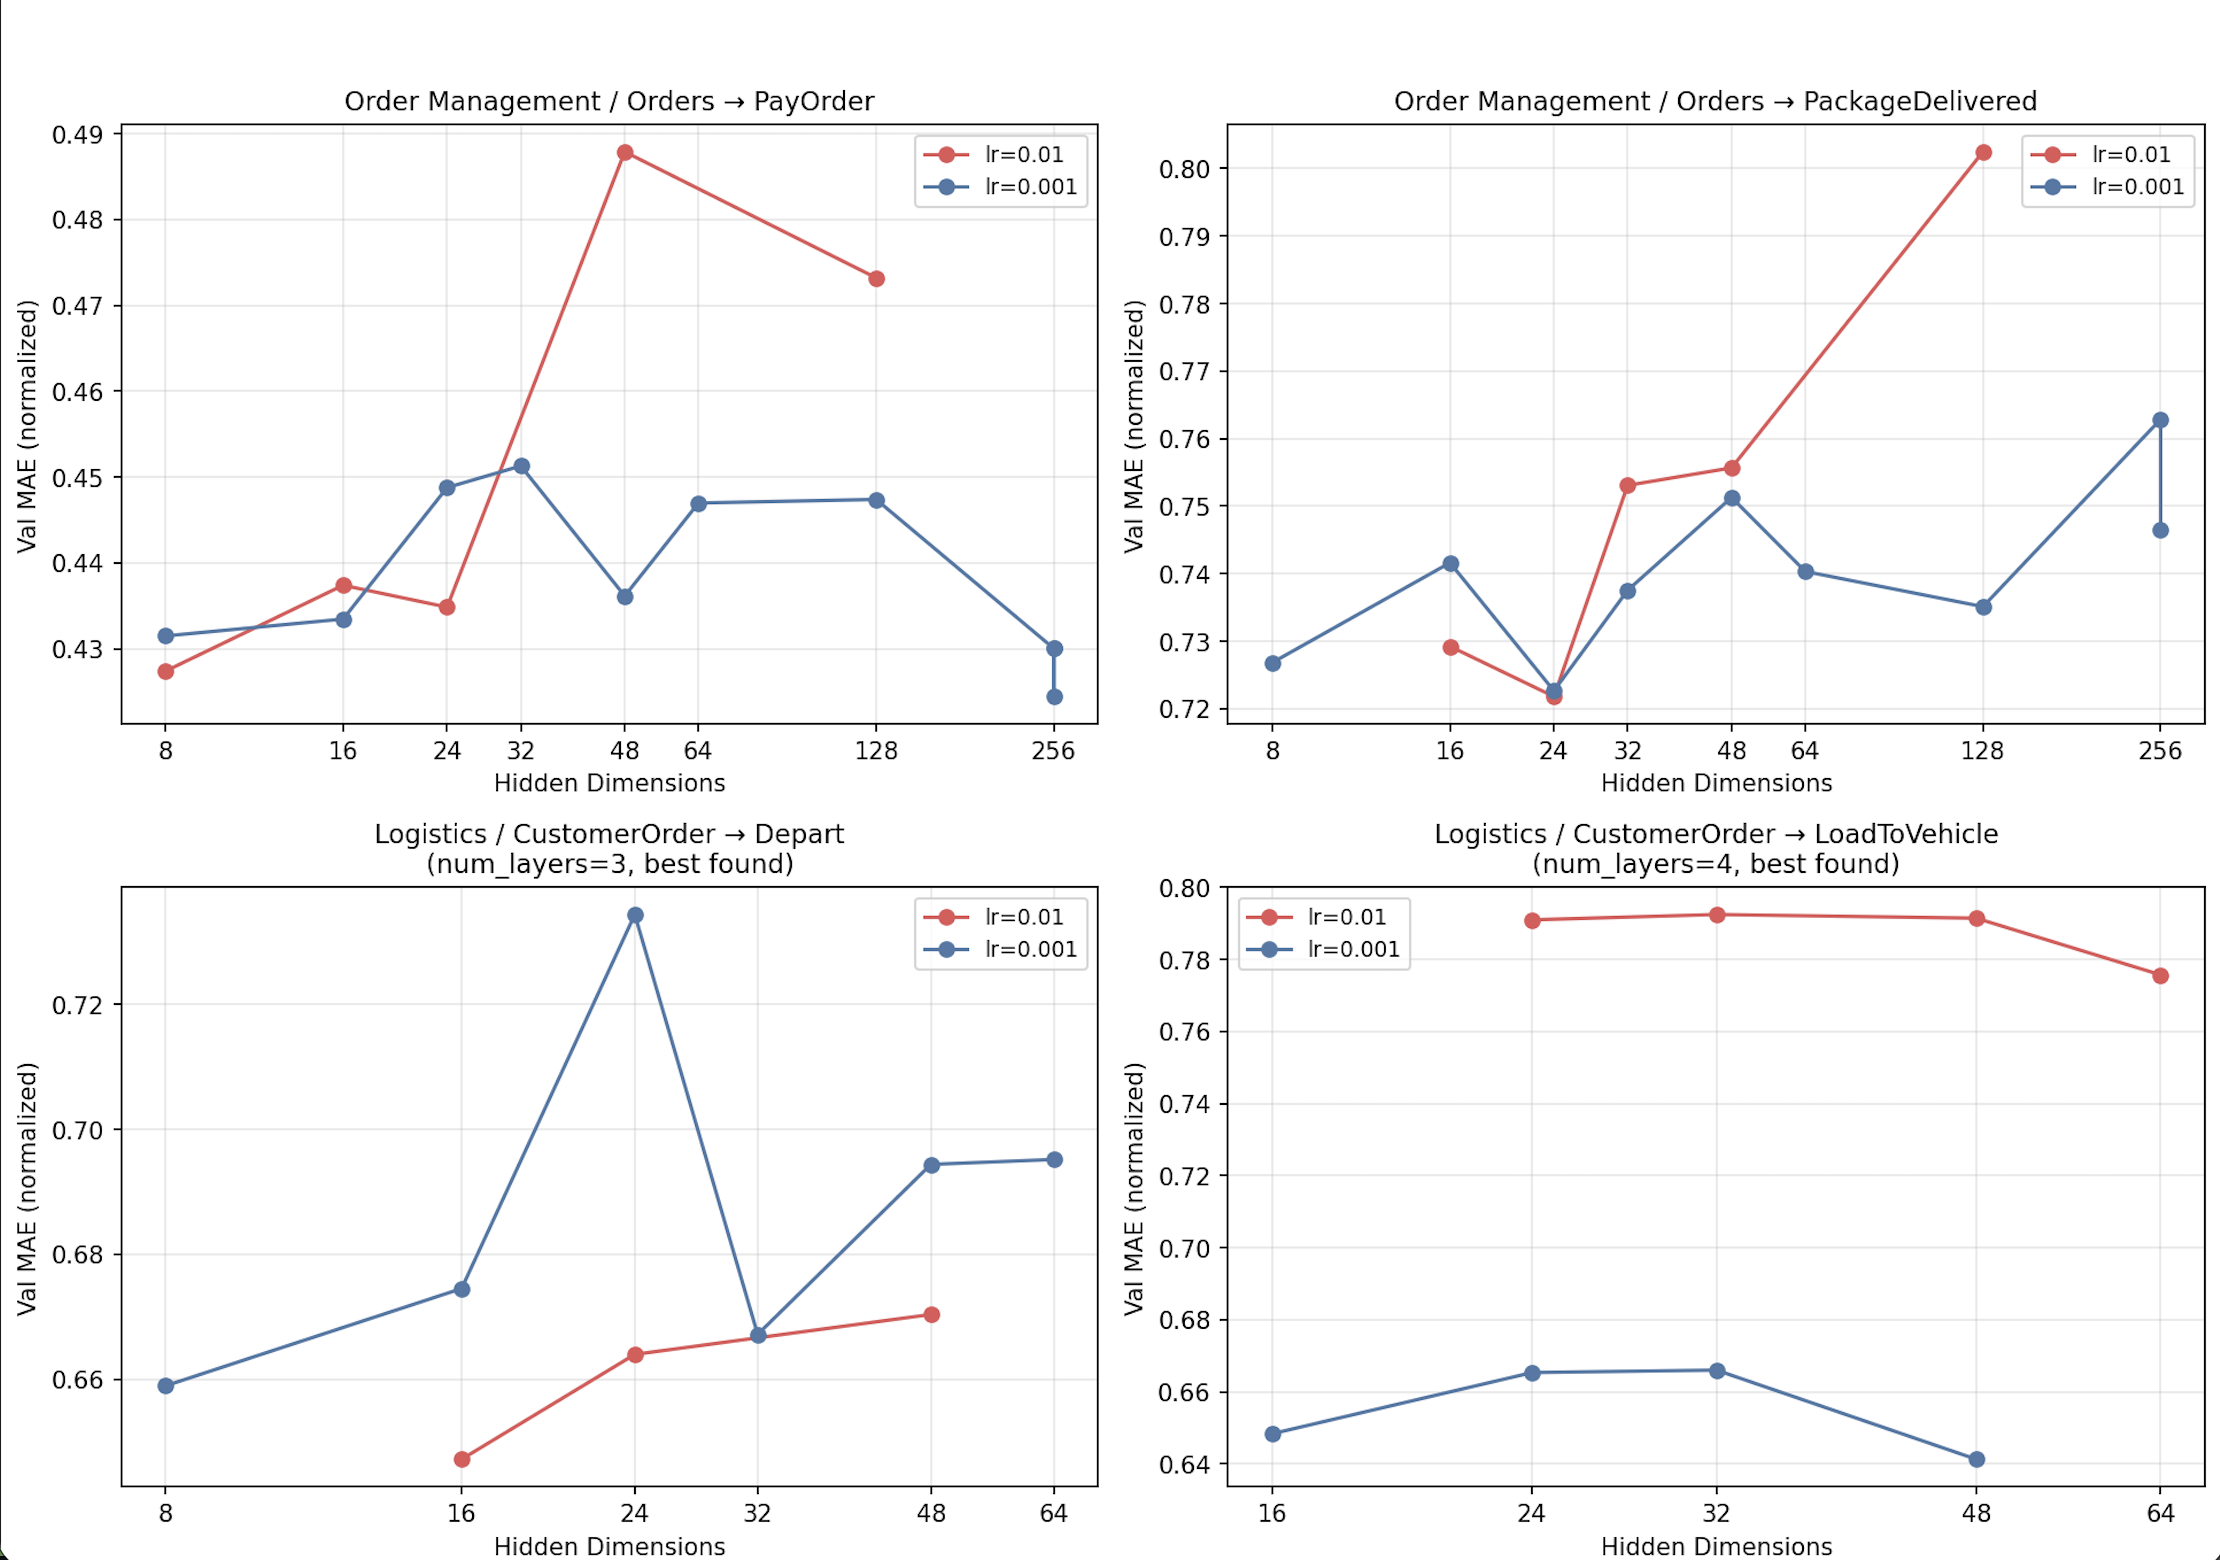
\includegraphics[width=1\textwidth]{figures/hyperparameter_sweep_summary.png}
                \caption{Normalized Val MAE scores for the HTG model per hyperparameter setting. Note: scales (y-axis) are not aligned, as I intended to compare hyperparameter settings within each KPI.}
                \label{fig:hyper_sweep}
            \end{figure}
            
            Fig. \ref{fig:hyper_sweep} shows the effect of tuning the learning rate and the number of hidden dimensions for the HGT regression models used. The graphs show the sweep for each of the four KPIs chosen, with "Orders -> PayOrder" representing the "Elapsed time from Orders to PayOrder" KPI (This nomenclature was used to avoid overloading the graphs with text) and the other three KPIs following the same style.
            
            Beginning with the two graphs shown at the top, referring to the Order Management KPIs, a first observation shows a great difference in volatility between the models' validation error when trained on the 0.01 learning rate versus the lower 0.001 value. The first continues increasing as more hidden dimensions are added, whereas the second is much more stable. It's important to note that the validation error is also higher for the "Elapsed time from Orders to PackageDelivered" KPI as opposed to the values shown for "Elapsed time from Orders to PayOrder" KPI. This could be a result of the difference in process execution length for each given KPI. A notable difference between each KPI model is the chosen hidden dimension value for their respective models, with the "Elapsed time from Orders to PackageDelivered" KPI showing better results with 24 hidden dimensions whereas the "Elapsed time from Orders to PayOrder" KPI showed the best results with the maximum 256 hidden dimensions.

            In order to perform the same sweep on the Logistics database it was first necessary to identify the proper number of layers needed to avoid the problem outlined in Section \ref{sec:dataset_logistics}.
            
            \begin{figure}[t!]
                \centering
                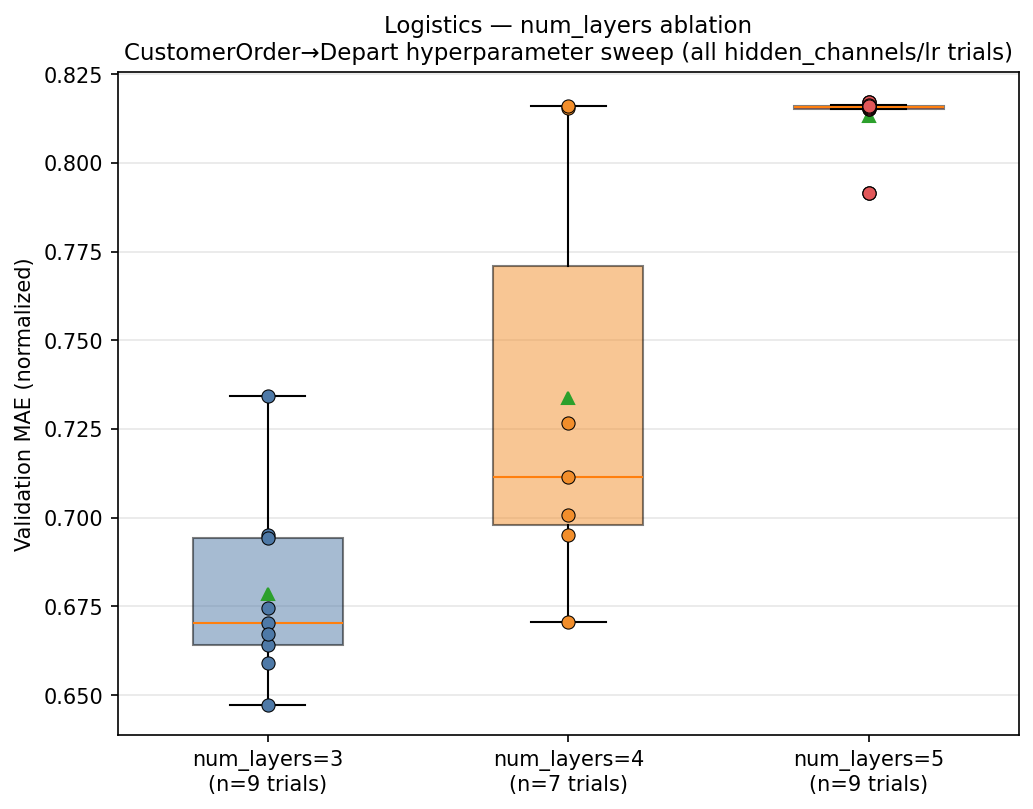
\includegraphics[width=1\textwidth]{figures/depart_ablation.png}
                \caption{Normalized Val MAE scores for the HGT model on the Logistics dataset for KPI "Elapsed time from CustomerOrder to Depart" per different number of layers}
                \label{fig:log_ablation_1}
            \end{figure}

            \begin{figure}[t!]
                \centering
                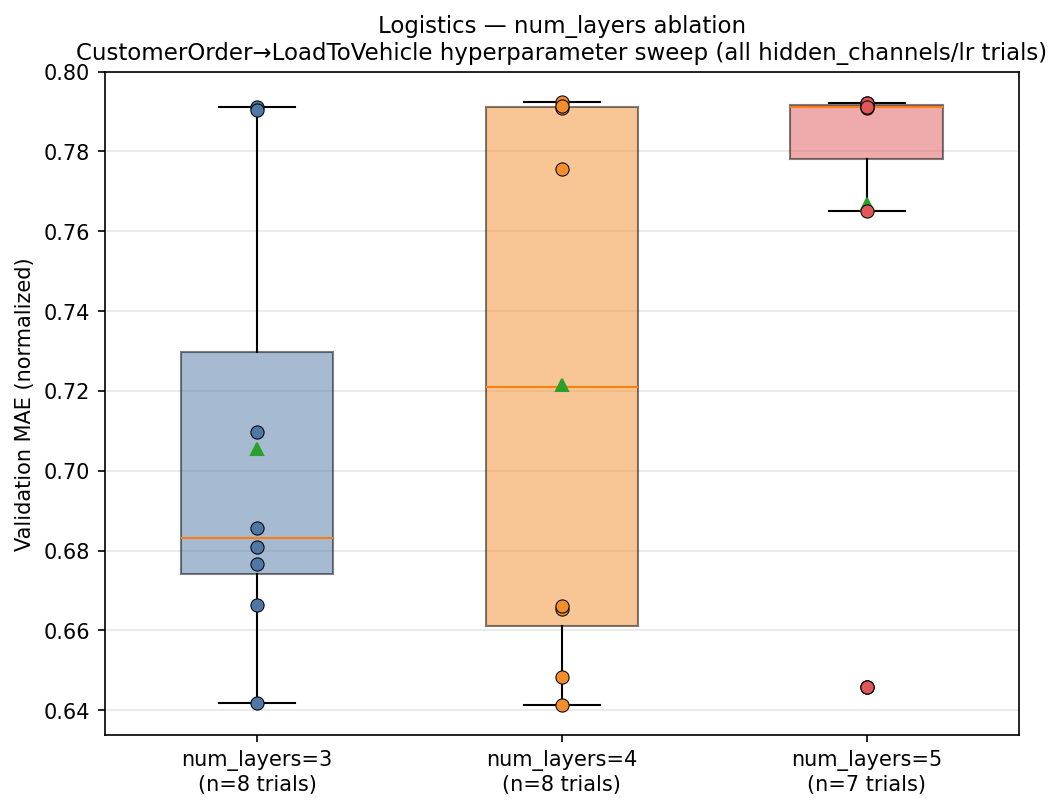
\includegraphics[width=1\textwidth]{figures/loadtovehcile_ablation.png}
                \caption{Normalized Val MAE scores for the HGT model on the Logistics dataset for KPI "Elapsed time from CustomerOrder to LoadToVehicle" per different number of layers}
                \label{fig:log_ablation_2}
            \end{figure}
            
            Fig. \ref{fig:log_ablation_1} and Fig. \ref{fig:log_ablation_2} show the result of the initial sweeps performed over all possible hidden channels and learning rates for each KPI in the Logistics dataset. In Fig. \ref{fig:log_ablation_1} it is evident that 3 layers offers the lowest overall validation error and the resulting sweep selected this value as the best hyperparameter. On the other hand Fig. \ref{fig:log_ablation_2} shows a different case, while the ablation analysis shows the number of layers at 3 having the best results, with its median at 0.683 versus the 0.721 of 4 layers, the complete sweep eventually selected 4 layers as the best option.

            The second set of graphs in Fig. \ref{fig:hyper_sweep} show the result of the sweep performed on the Logistics KPIs once the number of layers were set at the appropriate value of 3 and 4 respectively. It is important to note the different y-axis scales used by each graph as they are only intended for comparing setting within the model. Looking at the graph its evident that, in contrast to Order Management's results, the Logistics-trained models don't have a generally agreed upon set of hyperparameters characteristics. The "Elapsed time from CustomerOrder to Depart" KPI shows considerably better results when using a higher learning rate and a smaller number of hidden dimensions than either of the Order Management models. However, the sweep for "Elapsed time from CustomerOrder to LoadToVehicle" KPI shows a much flatter curve where the best values are provided by the lower learning rate and a hidden dimension value of 48.

        \subsection{Model comparison versus homogeneous GNN}
        \begin{figure}[t!]
            \centering
            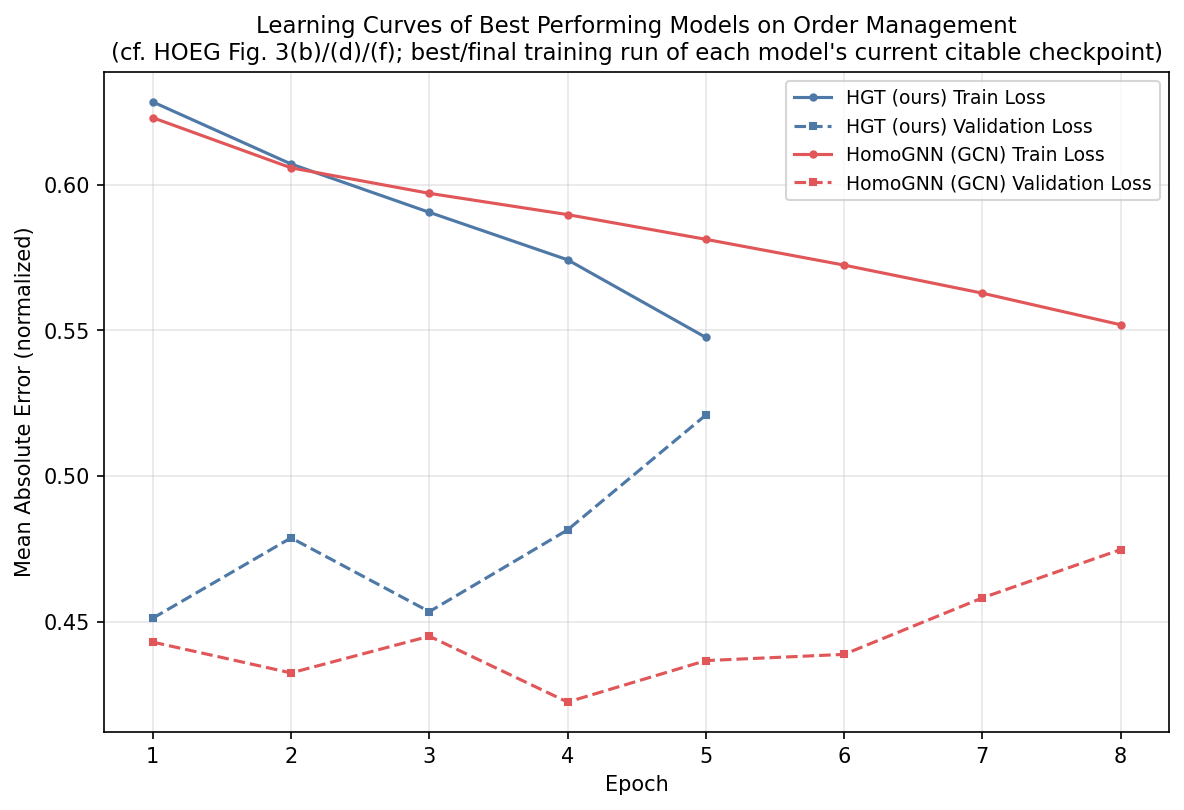
\includegraphics[width=1\textwidth]{figures/training_curves_order_management.png}
            \caption{Training and validation loss learning curves of the trained HGT model and the homogeneous GNN on the best performing model of the Order Management dataset.}
            \label{fig:learning_curves_om}
        \end{figure}
        
        Fig. \ref{fig:learning_curves_om} shows the learning curves for the best performing regression model on the Order Management dataset, which is associated with the prediction of the "Elapsed time from Orders to PayOrder" KPI. As can be seen in the curves, even after performing a hyperparameter sweep the model cannot be improved below a 0.45 MAE. Notably, training loss stays above validation loss for the entire run rather than the reverse, which at first glance suggests overfitting; however, re-evaluating the fully-trained checkpoint directly on each split (rather than reading the pattern off the epoch-by-epoch curve) shows train MAE (388.0 hours) is genuinely higher than validation MAE (353.2 hours), with test MAE the worst of the three (421.2 hours). 
        I then compared each split's target distribution directly, independent of any trained model, to validate whether this behavior was tied to the data source itself. I found the validation window's remaining-time values to be intrinsically less variable than the training window's (standard deviation of 135.8 hours versus 219.6 hours), so even a constant mean-predictor would score better on validation (105.7 hours MAE) than on training (158.1 hours MAE) suggesting temporal drift in the dataset.
        Test's higher error similarly reflects genuine temporal drift toward longer remaining times later in the dataset's timeline, not a generalization failure. Two candidate explanations for the pattern were checked directly and ruled out. The first was the possibility that the gap was caused by the z-normalization statistics being fit only on the training split. However, the denormalized MAE metric already corrects for this uniformly across splits so this explanation was discarded. Secondly, this pattern could be caused by too few training epochs. However, this explanation was also discarded since the gap traces to an intrinsic property of each split's data rather than an undertrained model. Training was still halted once the early-stop trigger activated after validation MAE stopped improving. The homogeneous implementation, which is allowed to train for longer, shows a similar overall pattern, with a decrease in training error not producing a decrease in validation error, instead increasing again after finding its local minimum at epoch 4 until it's also cut off by the early-stop trigger. Its smoother-looking curve does not translate into a clear performance advantage over the heterogeneous model for this KPI. HomoGNN's all-prefix MAE is slightly lower (157.5 hours versus 167.1 hours), but its last-event MAE remains higher than the heterogeneous model's (103.8 hours versus 98.0 hours). A full baseline comparison is presented later in this chapter that provides a complete picture across both metrics.

        

        \begin{figure}[t!]
            \centering
            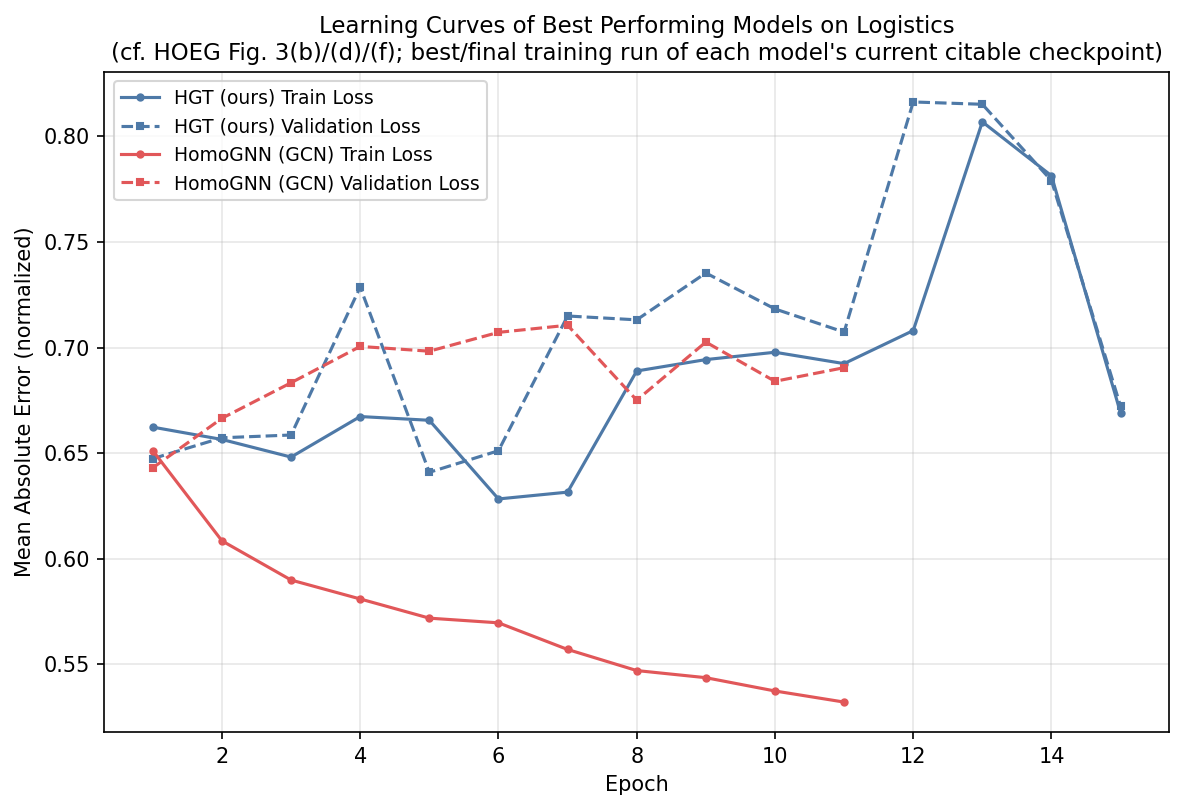
\includegraphics[width=1\textwidth]{figures/training_curves_logistics.png}
            \caption{Training and validation loss learning curves of the trained HGT model and the homogeneous GNN on the best performing model of the Logistics dataset.}
            \label{fig:learning_curves_log}
        \end{figure}

        Fig. \ref{fig:learning_curves_log} shows the learning curves for the best performing regression model on the Logistics dataset, which is associated with the prediction of the "Elapsed time from CustomerOrder to Depart" KPI. Both the homogeneous and heterogeneous models show a genuine overfitting-like divergence toward the end of the plotted run, with validation loss rising as training loss keeps dropping, and neither curve having visibly stabilized by the final epoch shown. 
        This divergence, however, occurs entirely after the epoch that early stopping actually selected. Logistics uses a patience of 10 epochs, so the plotted curve necessarily extends 10 epochs beyond the checkpoint that was saved and is cited elsewhere in this thesis, and it is in those extra, discarded epochs that training loss continues falling while validation loss rises. By reloading the actually-deployed checkpoint and re-evaluating it directly I confirmed that it does not carry this gap. Train, validation and test MAE are all within about 8 hours of each other (432.1h/435.1h/439.9h). Unlike what can be seen in the results for the order management dataset for this dataset the two models track each other closely throughout.

        Overall, neither graph reflects classic overfitting once the pattern behind it is more closely analyzed. Order Management's apparent gap is a property of its temporal validation split rather than a generalization failure, and Logistics' apparent divergence occurs only in training epochs beyond the one actually deployed. What both datasets do share is a training process that plateaus early, with the best available hyperparameters still leaving both model architectures at a relatively high absolute MAE floor for their respective KPIs.

        \subsection{Model comparison against baselines}
        \begin{figure}[t!]
            \centering
            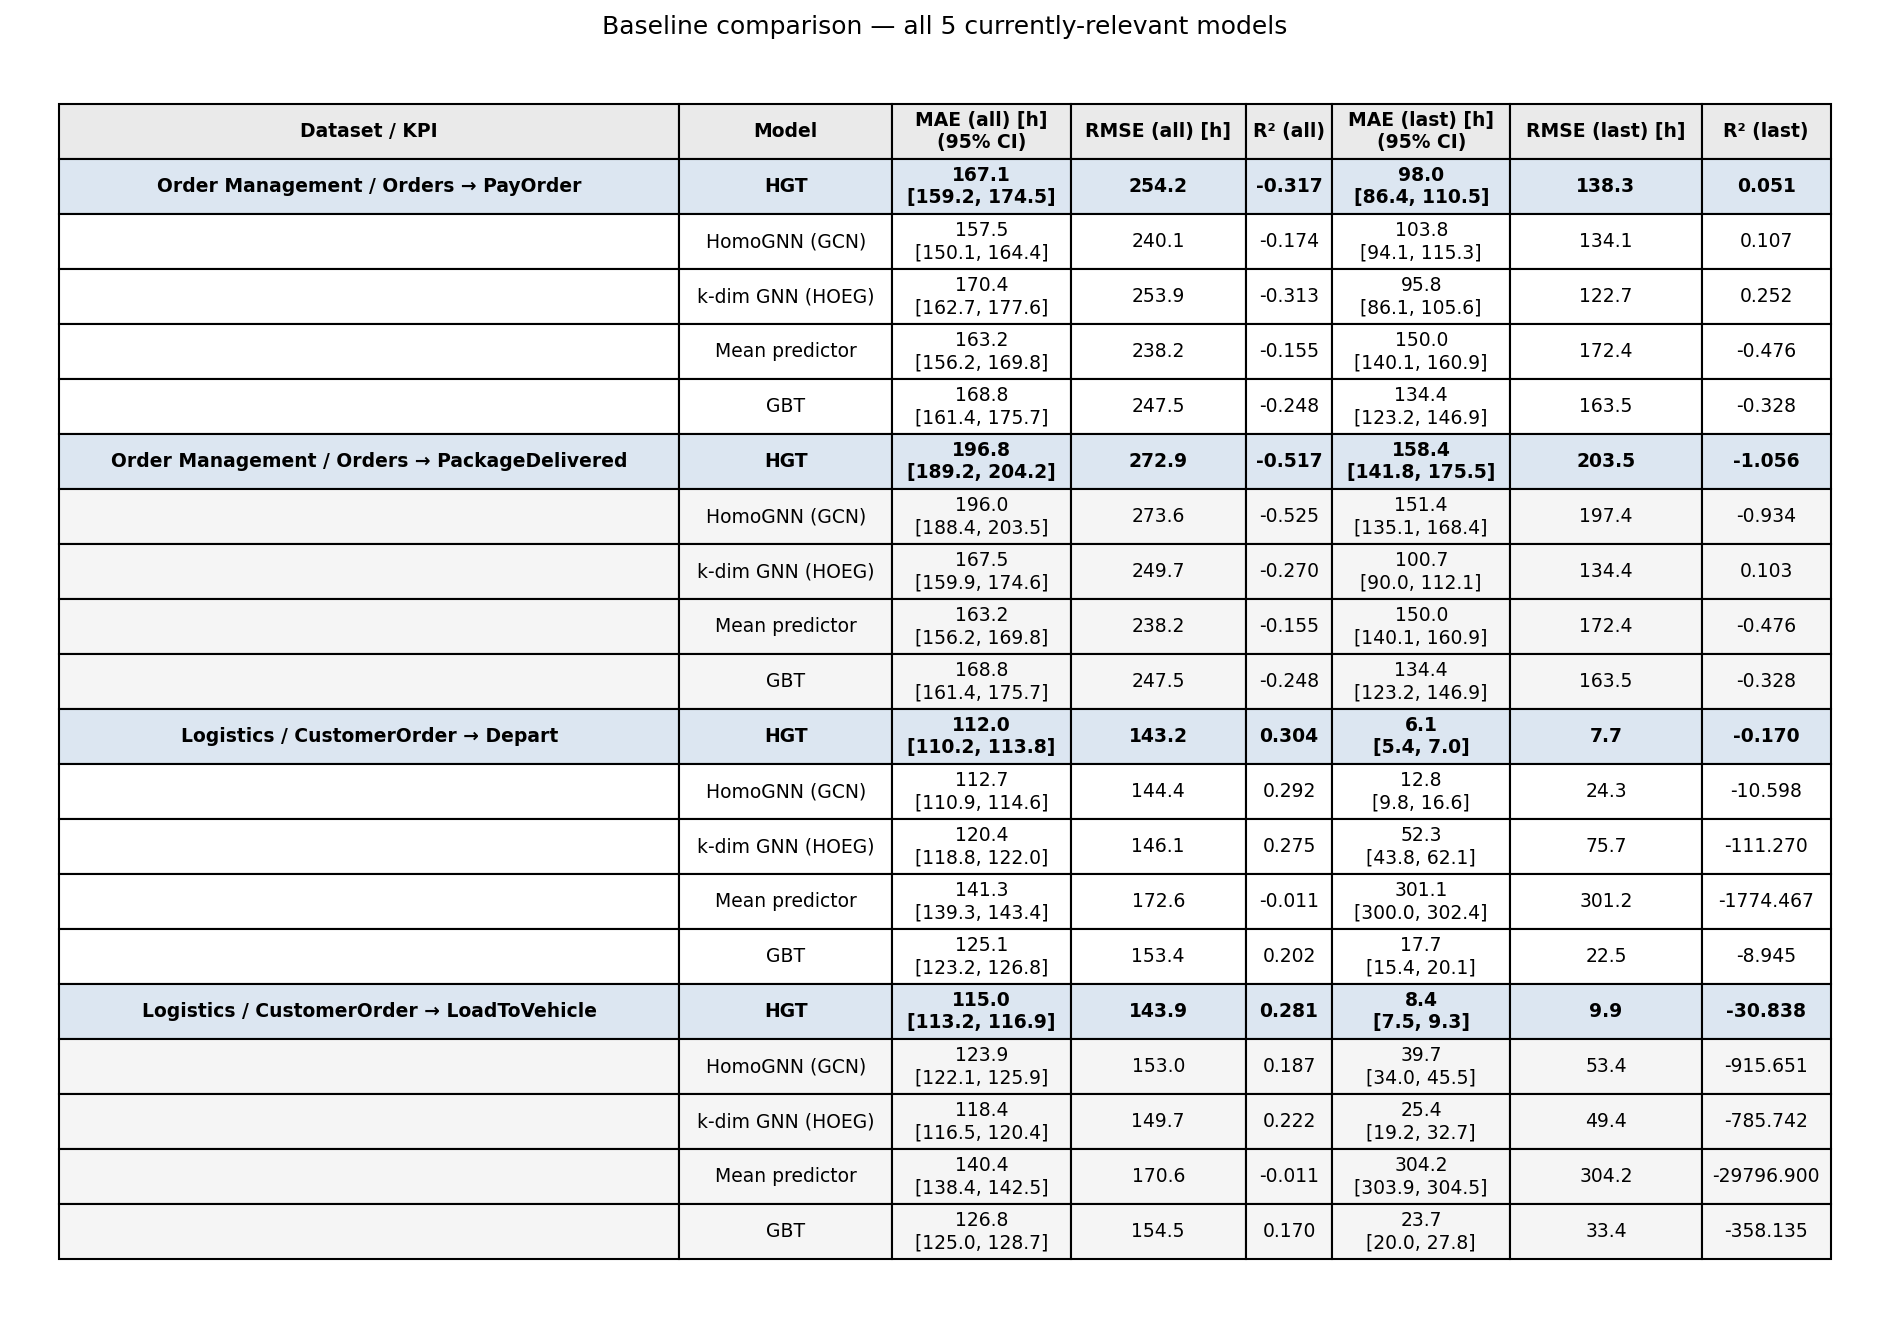
\includegraphics[width=1\textwidth]{figures/combined_baseline_comparison_table.png}
            \caption{Performance of the chosen HGT model and three baseline models. Note: the best-performing hyperparameter configurations are used for HGT}
            \label{fig:baselines}
        \end{figure}
        
        I compared the heterogeneous model against three other implementations: the mean, a Gradient Boosted Trees model and a homogeneous implementation of the dataset. By comparing the performance to these baseline models I wanted to understand how well the heterogeneous implementation stacked up to other options.
        Fig. \ref{fig:baselines} shows the results, with the MAE value denormalized and shown as hours. As I explained in Section \ref{sec:models_baselines} I was interested in checking the quality of the model not only on the entire prefix set but also as the prefix depth increased to evaluate if the increase in information was leading to an increase in predictive quality, Therefore, the graph presents the MAE values for both, the model tested on every prefix in the testing set as well as only those marked as Last-Event prefixes, which contain the maximum amount of information possible about the process execution.

As expected, the median estimator shows the worst overall performance for two of the four KPIs ("Time from CustomerOrder to Depart" and "Time from CustomerOrder to LoadToVehicle"). For the other two, however, it instead outperforms both the heterogeneous model and GBT: its error is slightly below both on "Time from Orders to PayOrder," and it is in fact the single best-performing model of the four on "Time from Orders to PackageDelivered." GBT's own performance is similarly inconsistent across KPIs rather than uniformly ranked: it is the single worst-performing model on PayOrder, the second-best (behind only the median estimator) on PackageDelivered, and mid-pack on the two Logistics KPIs, beating only the median estimator on each of those.
        Comparing the graph-based models it's clear that neither model can be identified as truly better than the other, with their respective accuracy values being very close. Looking at the confidence intervals of each model also shows that both models tend to have overlapping estimate ranges. Therefore, given the spread between models, it cannot be claimed with certainty that the heterogeneous representation is head-and-shoulders above the others — only that it is a reasonable, comfortable prediction.

        This changes if we compare the models only on the last-event prefix, though not as uniformly as it may first appear. For two of the four KPIs ("Time from CustomerOrder to Depart" and "Time from CustomerOrder to LoadToVehicle") the heterogeneous model is significantly more accurate than every baseline (Wilcoxon signed-rank p < 0.001 against each of the three baselines and the k-dim GNN comparison introduced in Section \ref{sec:models_baselines}). For "Time from Orders to PayOrder" it is significantly better than the homogeneous GNN, the mean predictor, and GBT, but statistically indistinguishable from the k-dim GNN baseline (p=0.31). For "Time from Orders to PackageDelivered," the heterogeneous model does not win at all: it is statistically tied with the homogeneous GNN (p=0.48) and significantly less accurate than the mean predictor, GBT, and the k-dim GNN baseline. 
        One further caveat applies on top of this for "Time from CustomerOrder to LoadToVehicle" KPI, which has a strongly negative $R^2$ for every model, most extremely for the mean predictor (R²=-29796). This is a consequence of the last-event target's true scale being tiny, with a mean of 2.3 hours and a standard deviation of only 1.8 hours (an order of magnitude smaller than the other Logistics KPI, which has a mean of 27 hours and a standard deviation of 7 hours). Since $R^2$ is calculated against this tiny variance, even the heterogeneous model's own comparatively modest last-event error produces a negative R² (-30.8)smaller in magnitude than the baselines' because its MAE is itself the lowest of the five, but still negative for the same structural reason. Overall, MAE remains the more informative metric for this KPI. As shown above, the heterogeneous model's last-event MAE is significantly lower than every baseline's here, unlike the mixed picture for PayOrder and PackageDelivered.

        \begin{figure}[t!]
            \centering
            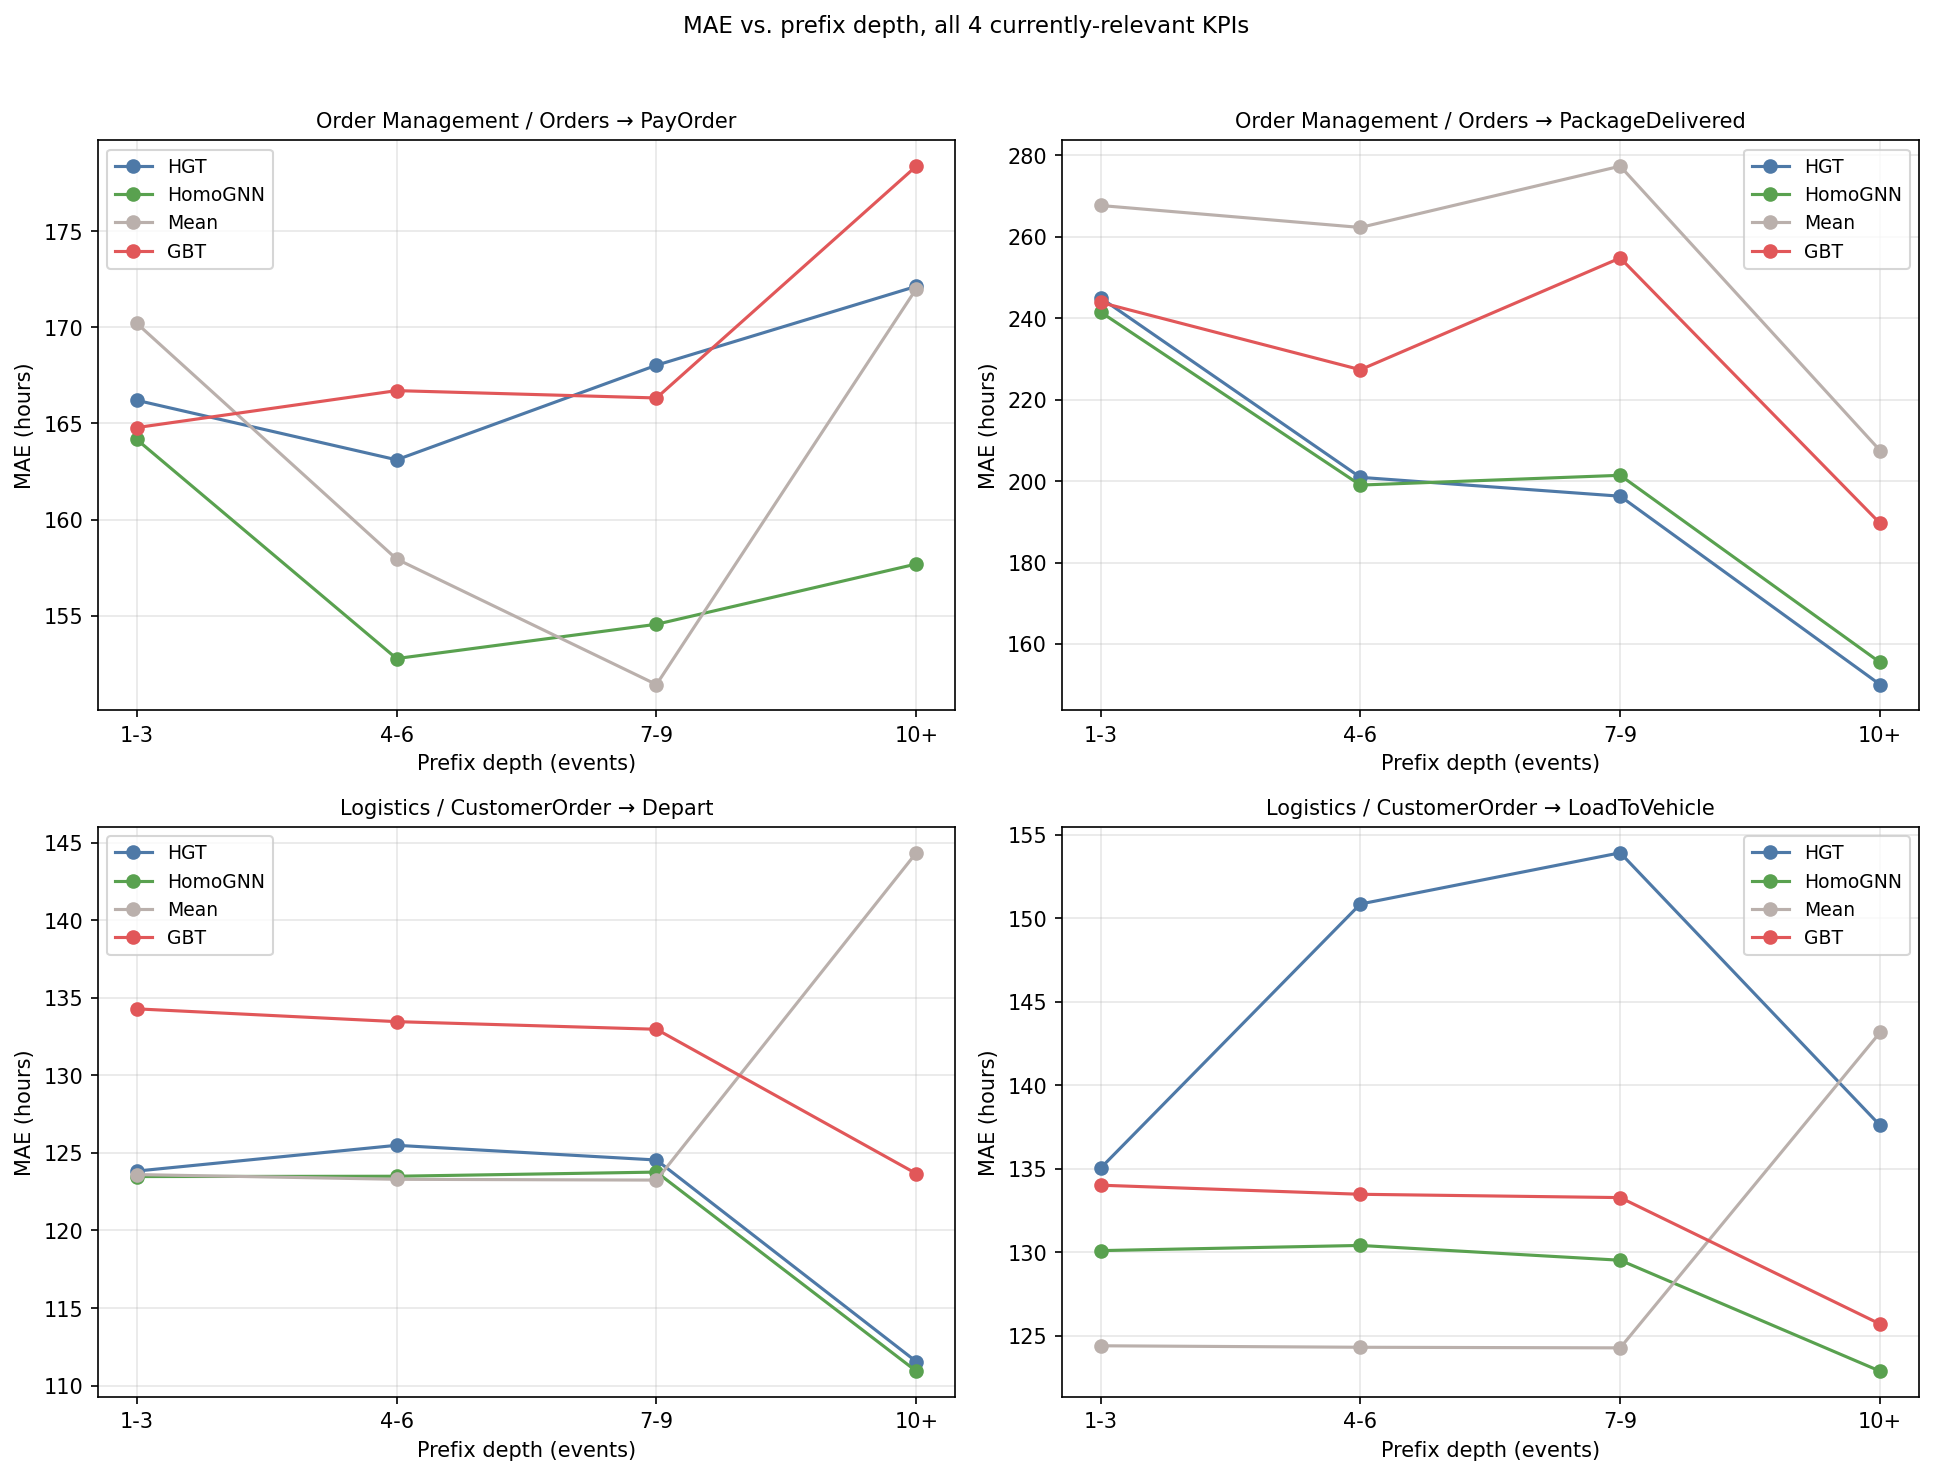
\includegraphics[width=1\textwidth]{figures/mae_by_depth_summary.png}
            \caption{Test MAE for each regression model across prefix depth.}
            \label{fig:depth_summary}
        \end{figure}
        
        Fig. \ref{fig:depth_summary} shows this change in predictive quality over prefix depth. The graphs show that in only two of the four KPIs the model's performance works as expected, with the MAE value decreasing as more information is added to the process execution. The HGT model for the "Time from CustomerOrder to LoadToVehicle" KPI is especially problematic as it's the only model that increases across the prefix depth.
        These graphs also highlight an important result. The HGT model used performs worse for three of the four regression models, with its MAE always higher than the homogeneous model's across multiple prefix depths. 
        This result reverses for two of the four KPIs when comparing the models exclusively on last-event prefixes, as shown in the statistical breakdown above, indicating that aggregate metrics, which are dominated by non-last-event prefixes, and last-event-specific metrics can move independently, sometimes in opposite directions. However, it is worth noting that the aformentioned breakdown also shows this reversal is itself KPI-dependent rather than universal.

    \section{Explainability framework}
        Having described the predictive model's results I now show the results of applying my proposed explainability framework on the created models. I show the output of each of the four distinct components of the framework as well as a short explanation of how the provided explanations can be interpreted by a stakeholder.

        \subsection{Perturbation-based explanation}
            \begin{figure}[t!]
                \centering
                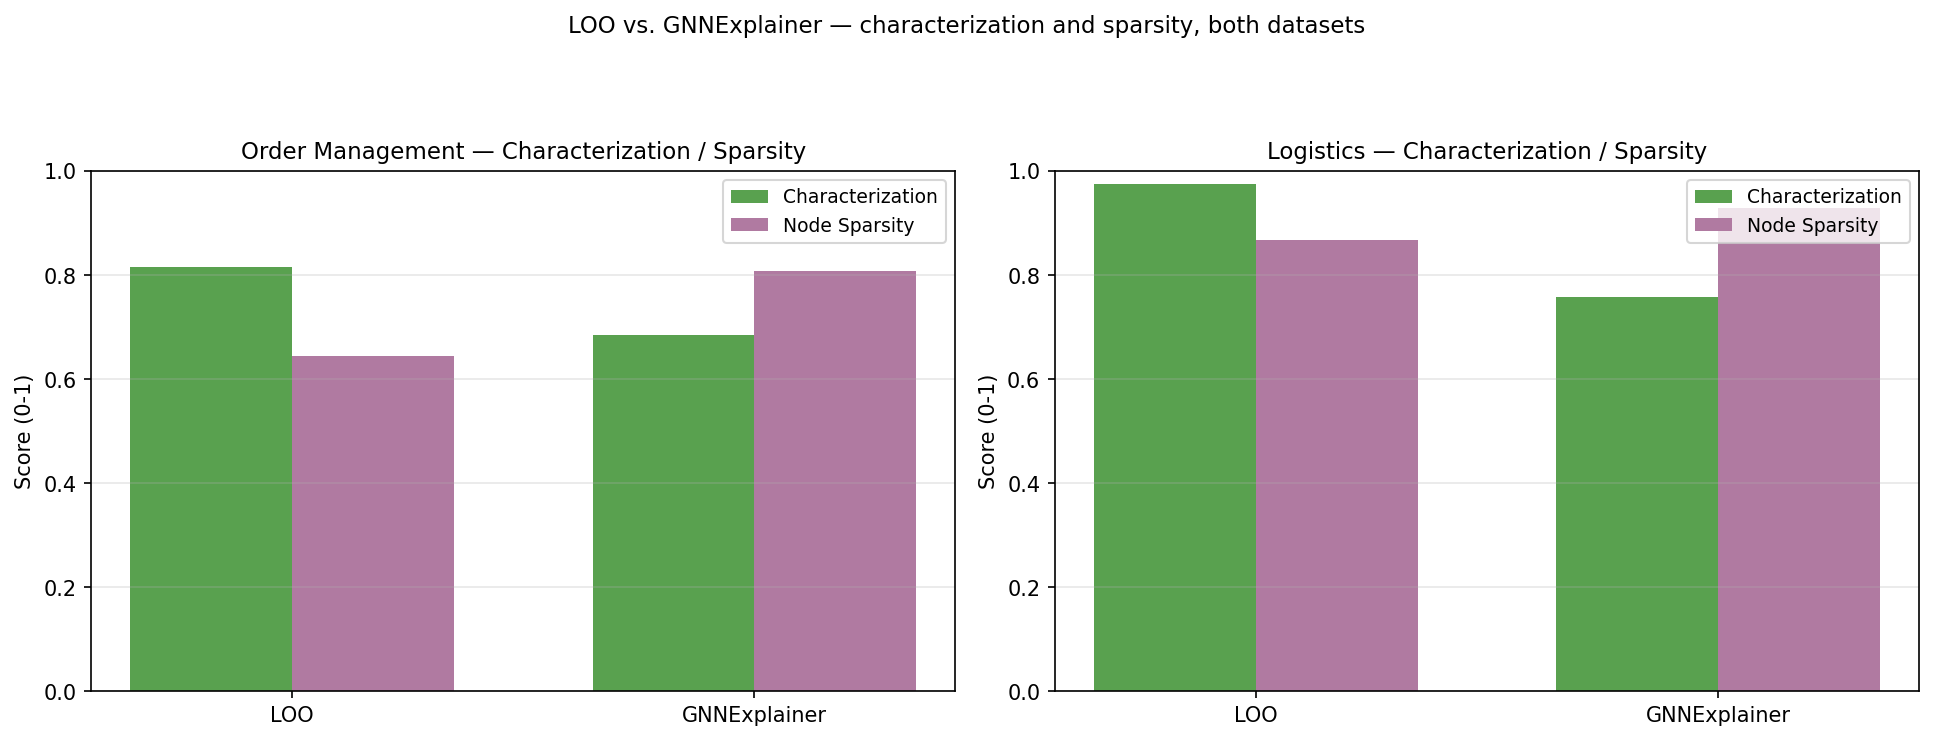
\includegraphics[width=1\textwidth]{figures/fidelity_comparison_summary.png}
                \caption{Fidelity metrics of LOO method against GNNExplainer for KPIs of each dataset}
                \label{fig:loo_comparison}
            \end{figure}
            
			As I explained in Section \ref{sec:dataset_perturb} I performed a series of tests to validate a change in the way this part of the methodology generated its results. Fig. \ref{fig:loo_comparison} shows the results of this evaluation. I compared the two methods on two explanation fidelity metrics: characterization and sparsity. As can be seen LOO outperformed GNNExplainer on both metrics across both datasets (characterization: Order Management LOO 0.815 vs. GNNExplainer 0.685; Logistics LOO 0.975 vs. GNNExplainer 0.757), meaning that features identified through LOO lead to better fidelity metrics compared to those found by the heterogeneous implementation of GNNExplainer. Logistics' characterization score is, in fact, the higher of the two datasets rather than the lower one, indicating that LOO-identified features are highly decisive for the model's prediction in both settings.

            \begin{figure}[t!]
                \centering
                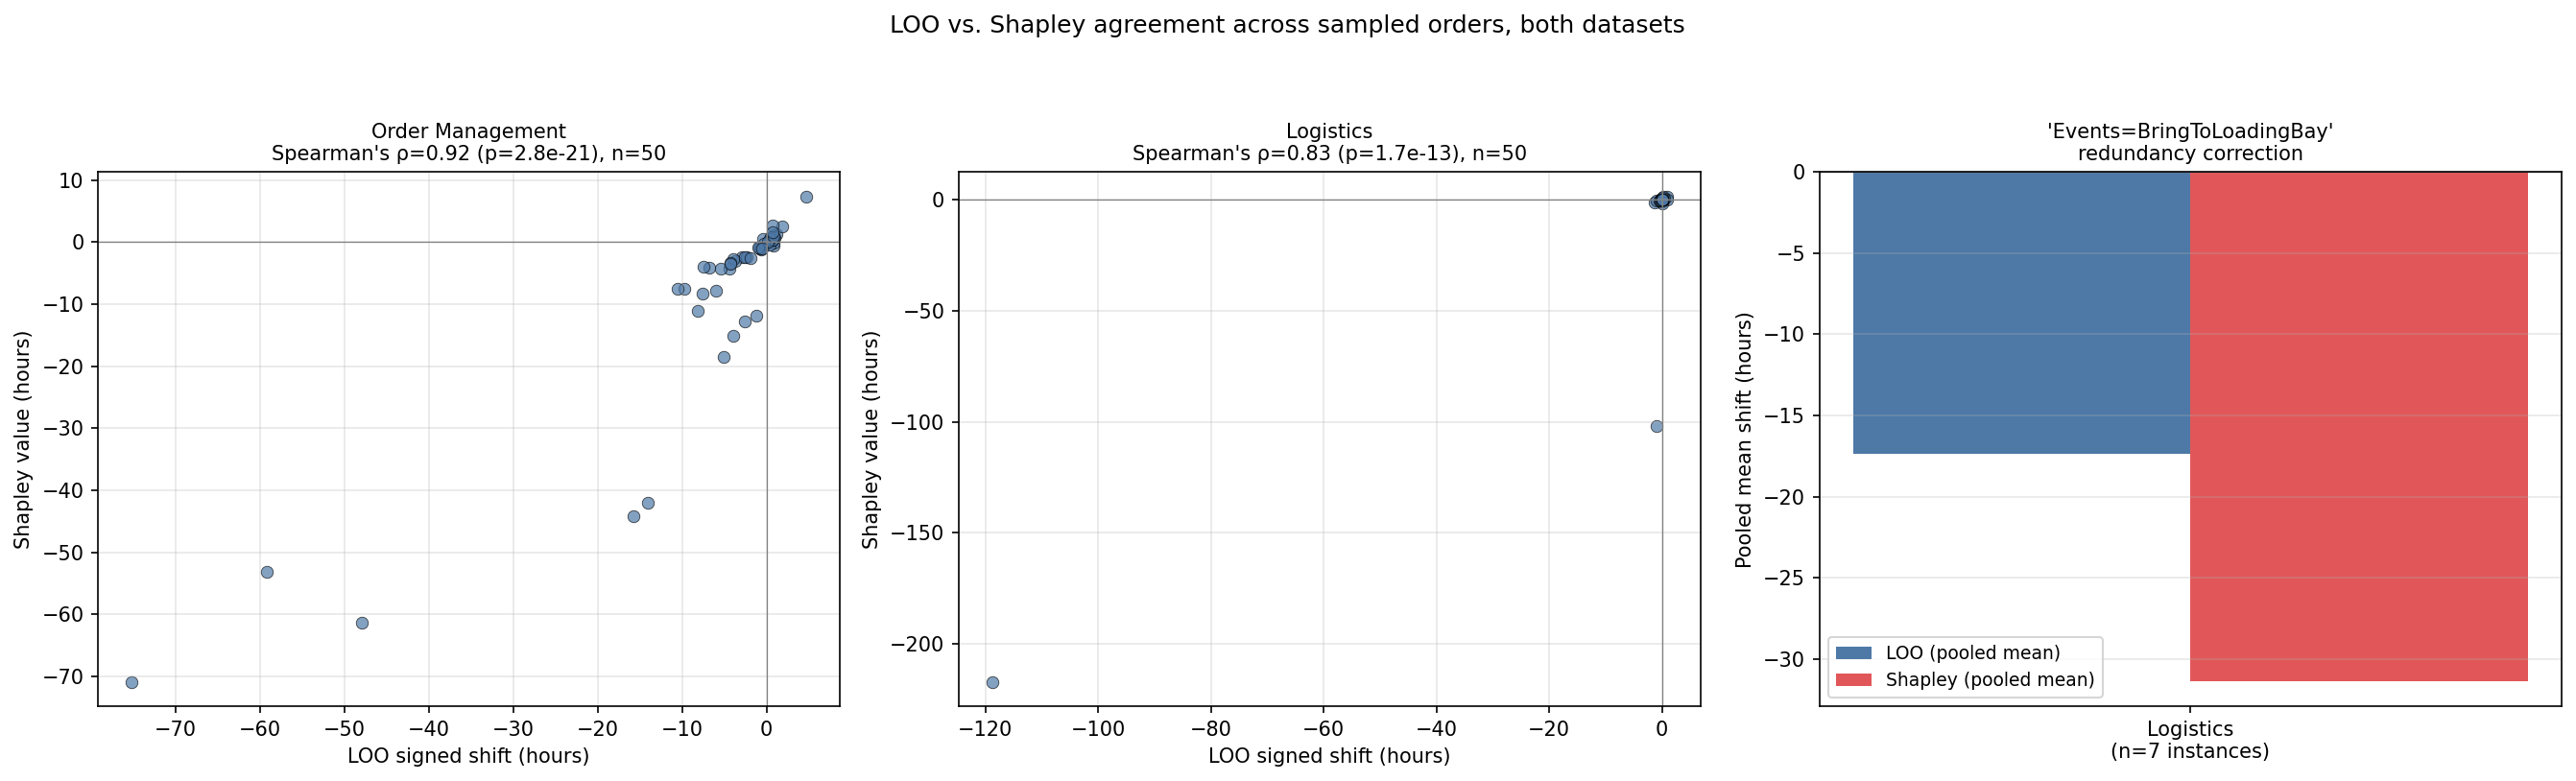
\includegraphics[width=1\textwidth]{figures/loo_vs_shapley_agreement.png}
                \caption{Measure of agreement between LOO method and full Shapley Values}
                \label{fig:loo_shapley_comp}
            \end{figure}
            
			Additionally, I needed to validate LOO's effectiveness as a proper identifier to limit the space over which Shapley Values would need to be run. Fig. \ref{fig:loo_shapley_comp} shows the result of this analysis. Both datasets show a strong, statistically significant rank agreement between the values identified by the two methods: Order Management reported a Spearman's $\rho$ value of 0.92 (p=2.8e-21), and Logistics reported a value of 0.83 (p=1.7e-13), each over 50 sampled orders. Despite this strong agreement in ranking, the two methods can still disagree on an element's exact magnitude when its underlying occurrences are redundant with one another. Logistics' \texttt{BringToLoadingBay} event, which recurs multiple times within a single process execution, illustrates this: LOO's pooled mean shift across the 7 instances where it appears is -17.3 hours, while Shapley's coalition-based accounting attributes -31.3 hours to the same event, correcting for the redundancy between its repeated occurrences that LOO's one-at-a-time removal underestimates. This highlights the continued need for Shapley Values as a proper quantifying method even where LOO's ranking alone is a reliable and much cheaper identifier.

            \begin{figure}[t!]
                \centering
                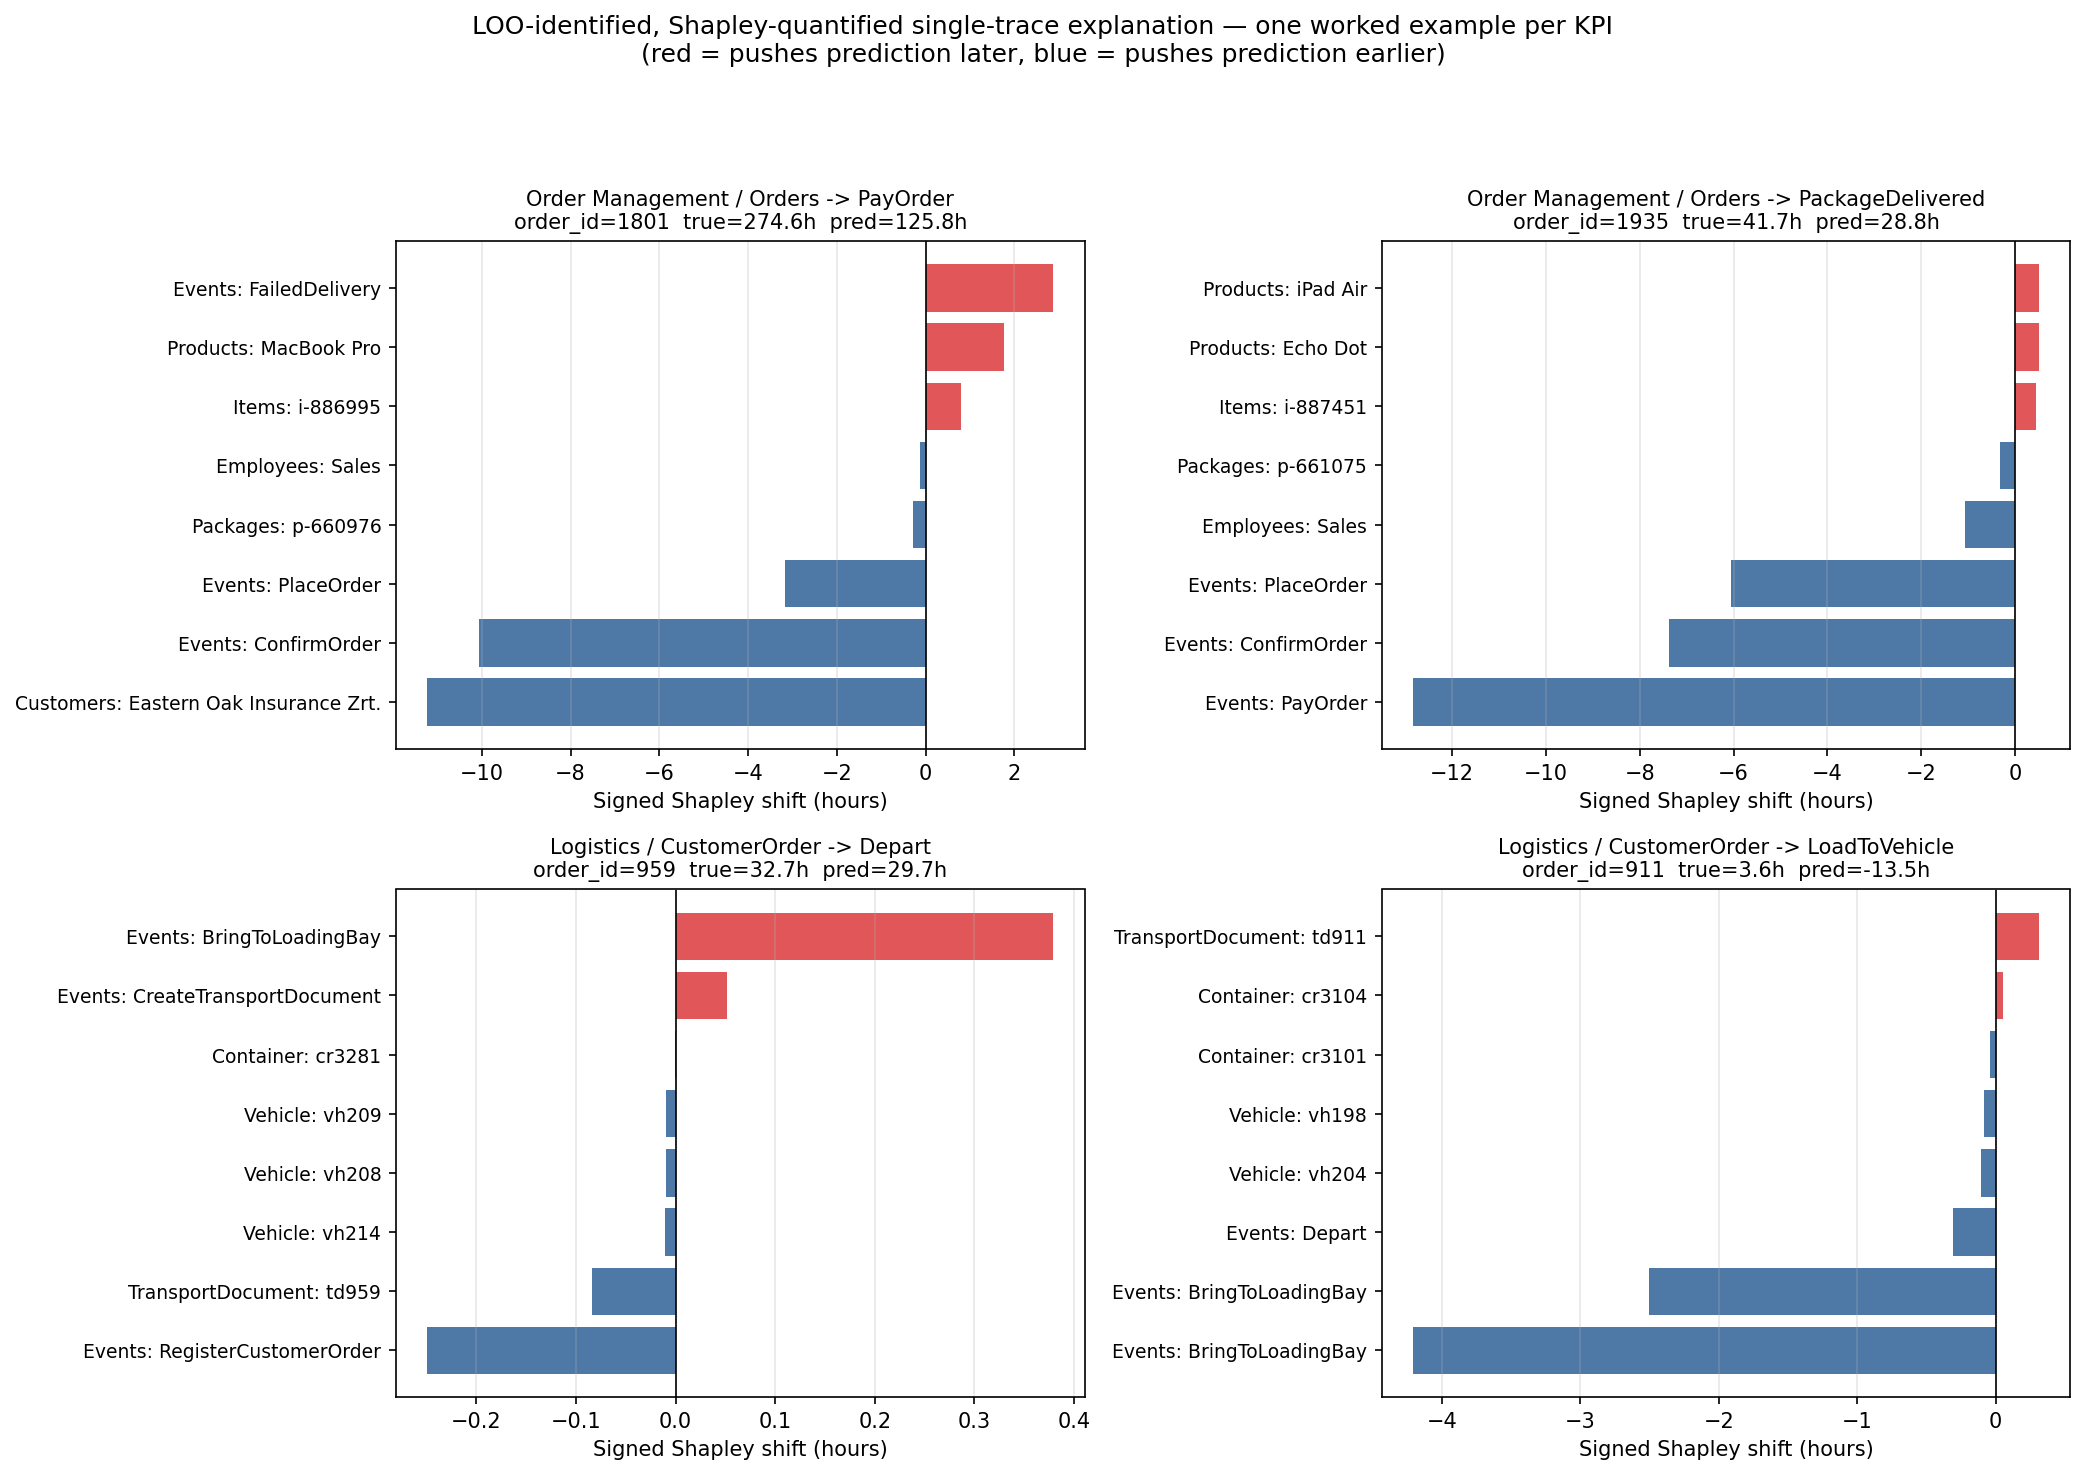
\includegraphics[width=1\textwidth]{figures/loo_shapley_trace_showcase.png}
                \caption{Graphs showing the single-trace explanations generated indicating the most important nodes in each trace as well as the impact on the model's prediction.}
                \label{fig:loo_shapley_showcase}
            \end{figure}

            \begin{figure}[t!]
                \centering
                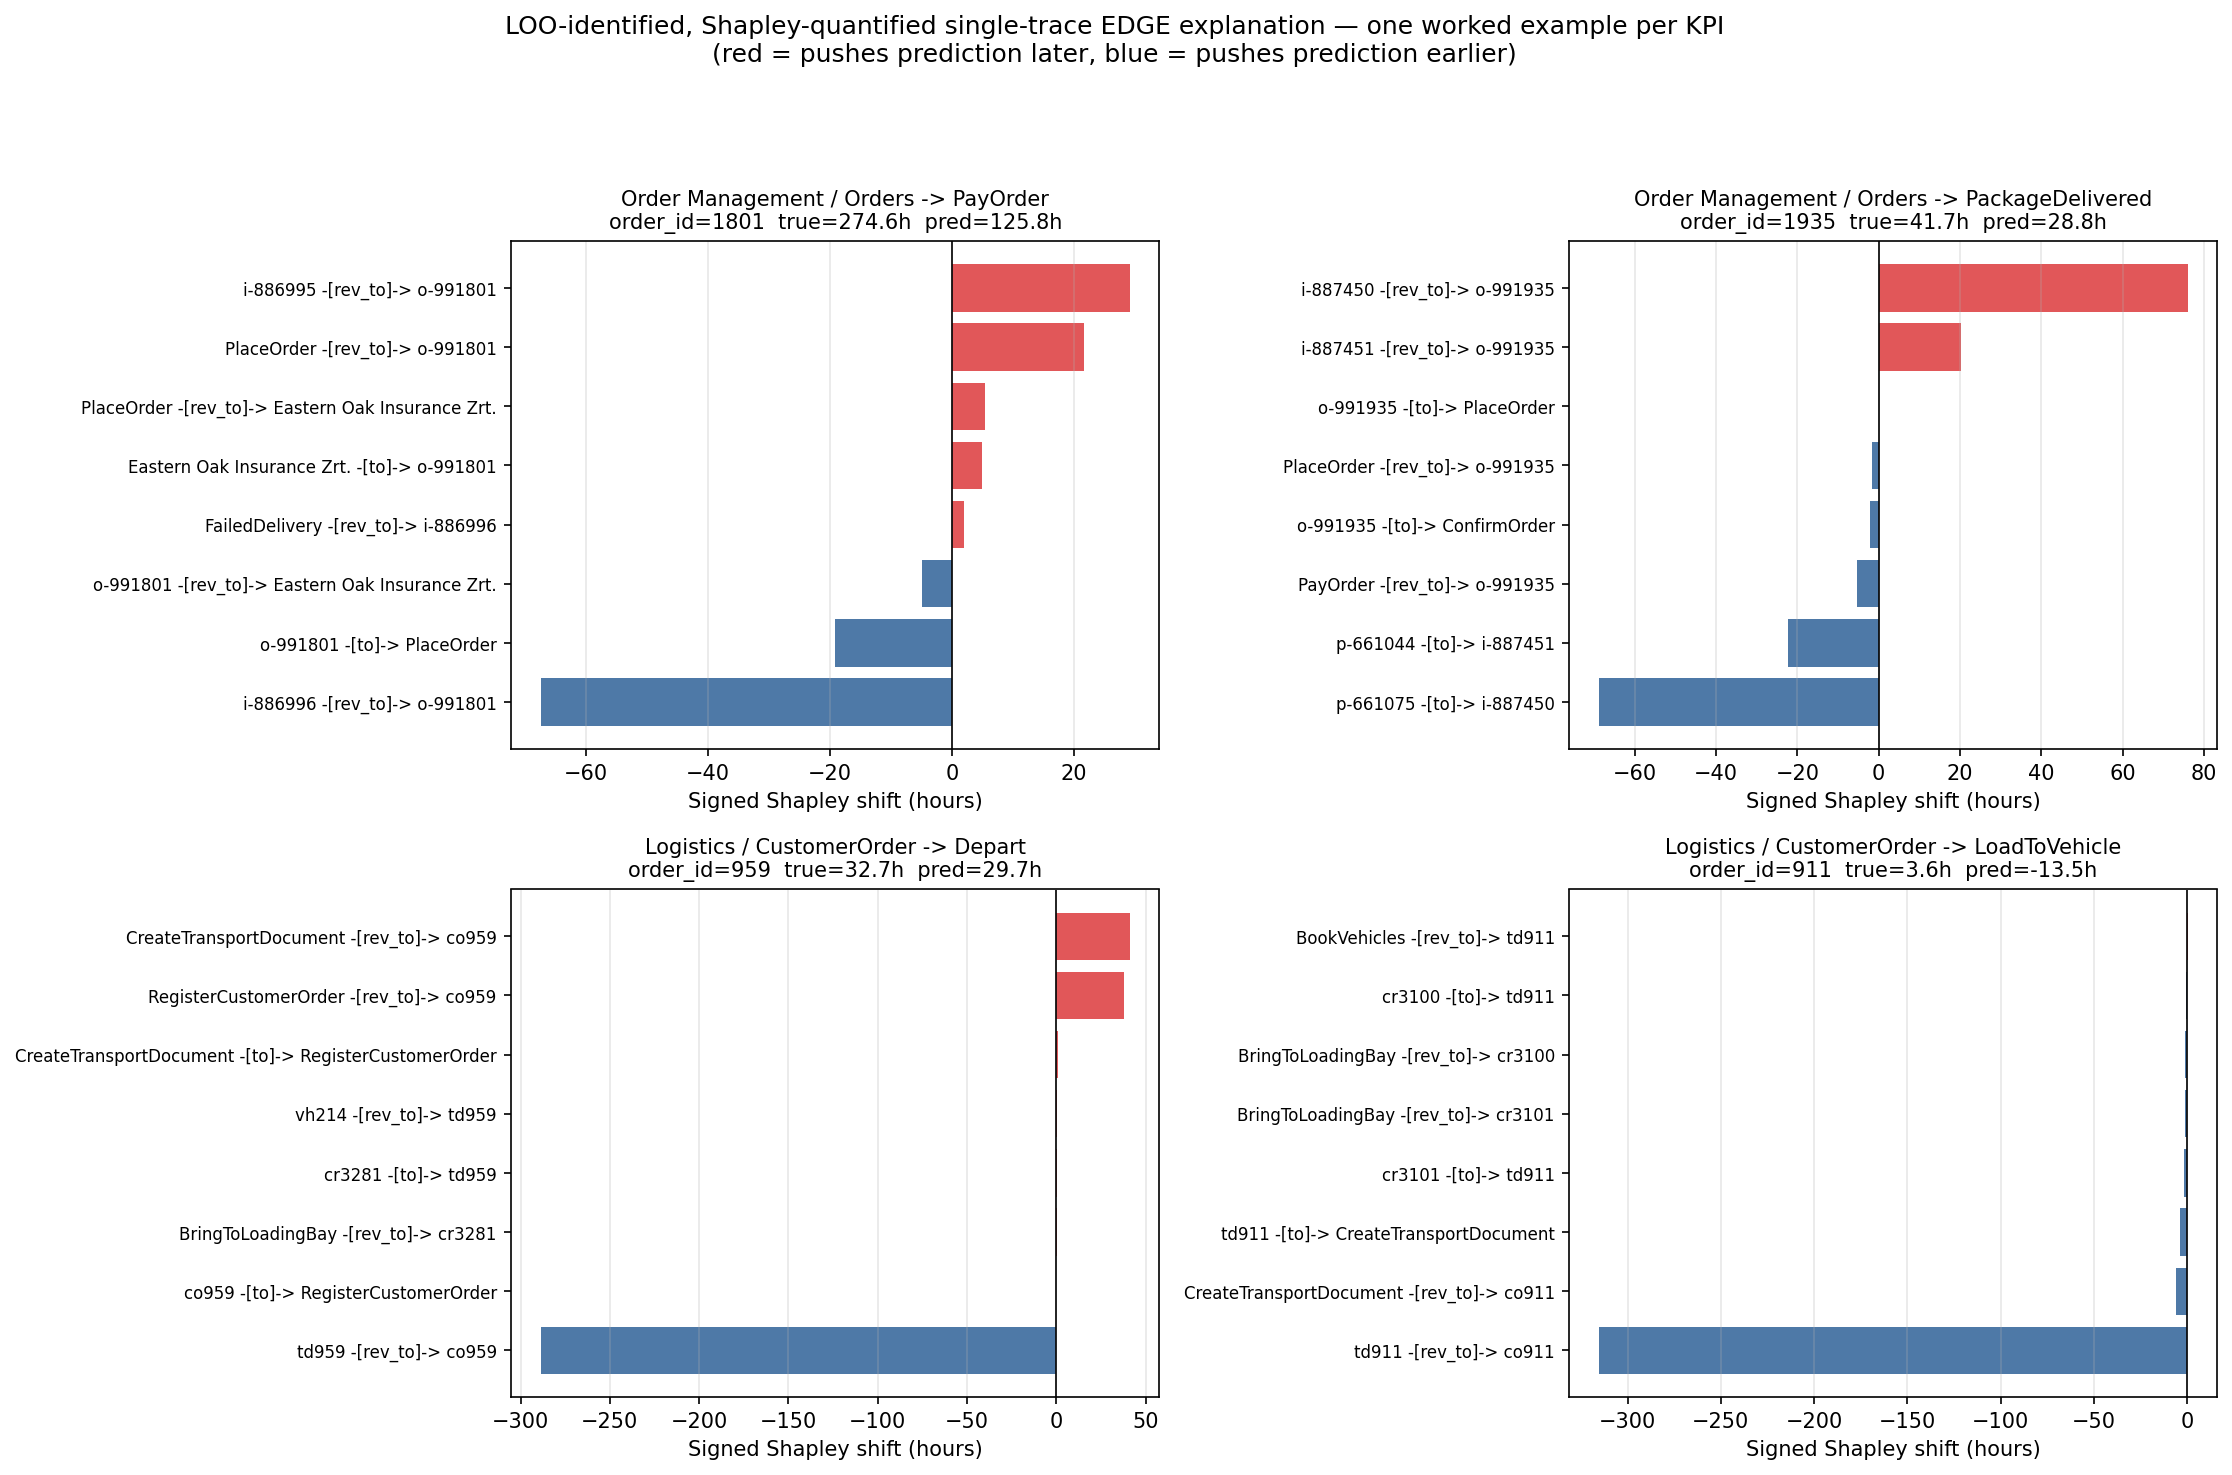
\includegraphics[width=1\textwidth]{figures/loo_shapley_edge_trace_showcase.png}
                \caption{Graphs showing the single-trace explanations generated indicating the most important edges in each trace as well as the impact on the model's prediction.}
                \label{fig:loo_edge_showcase}
            \end{figure}
            
            Before working through these examples, it is worth being explicit about how the single trace shown in them was chosen. Every single-trace figure in this section, as well as the gradient-based and counterfactual explanations shown later in this chapter, reuses the same order (order 1801, Order Management dataset, Orders $\to$ PayOrder) as one running example, rather than a fresh trace per figure. This is a deliberate choice made for narrative continuity, not a claim that the trace is representative: order 1801 was originally selected via a "slow trace" heuristic (a trace from the bottom quintile by remaining time, chosen to make for an interesting worked example), with no accuracy or fidelity criterion involved in its selection, and its own explanation fidelity later in this chapter turns out to be below the dataset average rather than favorably cherry-picked (Fig. \ref{fig:fidelity_graph}, characterization 0.565 against an aggregate LOO characterization of 0.815, Fig. \ref{fig:loo_comparison}). The dataset-wide, representative picture instead comes from the holistic aggregate view at the end of this section (Figs. \ref{fig:agg_shapley_global_om_payorder}-\ref{fig:agg_shapley_global_logistics_loadtovehicle}), which pools hundreds of predictions rather than illustrating a single one.

            Fig. \ref{fig:loo_shapley_showcase} shows examples of the graphs shown to the stakeholder for the single trace perturbation-based explanation. As can be seen the provided graphs show the node type and it's associated OCEL identifier. The node's impact on the model's prediction is shown in terms of hours, a proper understandable magnitude the stakeholder can interpret, with bar size and color showing the magnitude of the impact and its sign respectively, All this elements are considered in order to make the presented explanation as easily interpretable as possible by a stakeholder with limited knowledge about the workings of the predictive model. Additionally, the stakeholder is also provided with a table that gives a more structured view of the same information as the graphs.
			The presented analysis is applied to the three components of the input graph (nodes, edges and their associated feature values), each graph and table providing a summary of the information for each of these elements. Fig. \ref{fig:loo_edge_showcase} shows the same explanation process applied to the edges of prefixes in each dataset.

            \begin{figure}[t!]
                \centering
                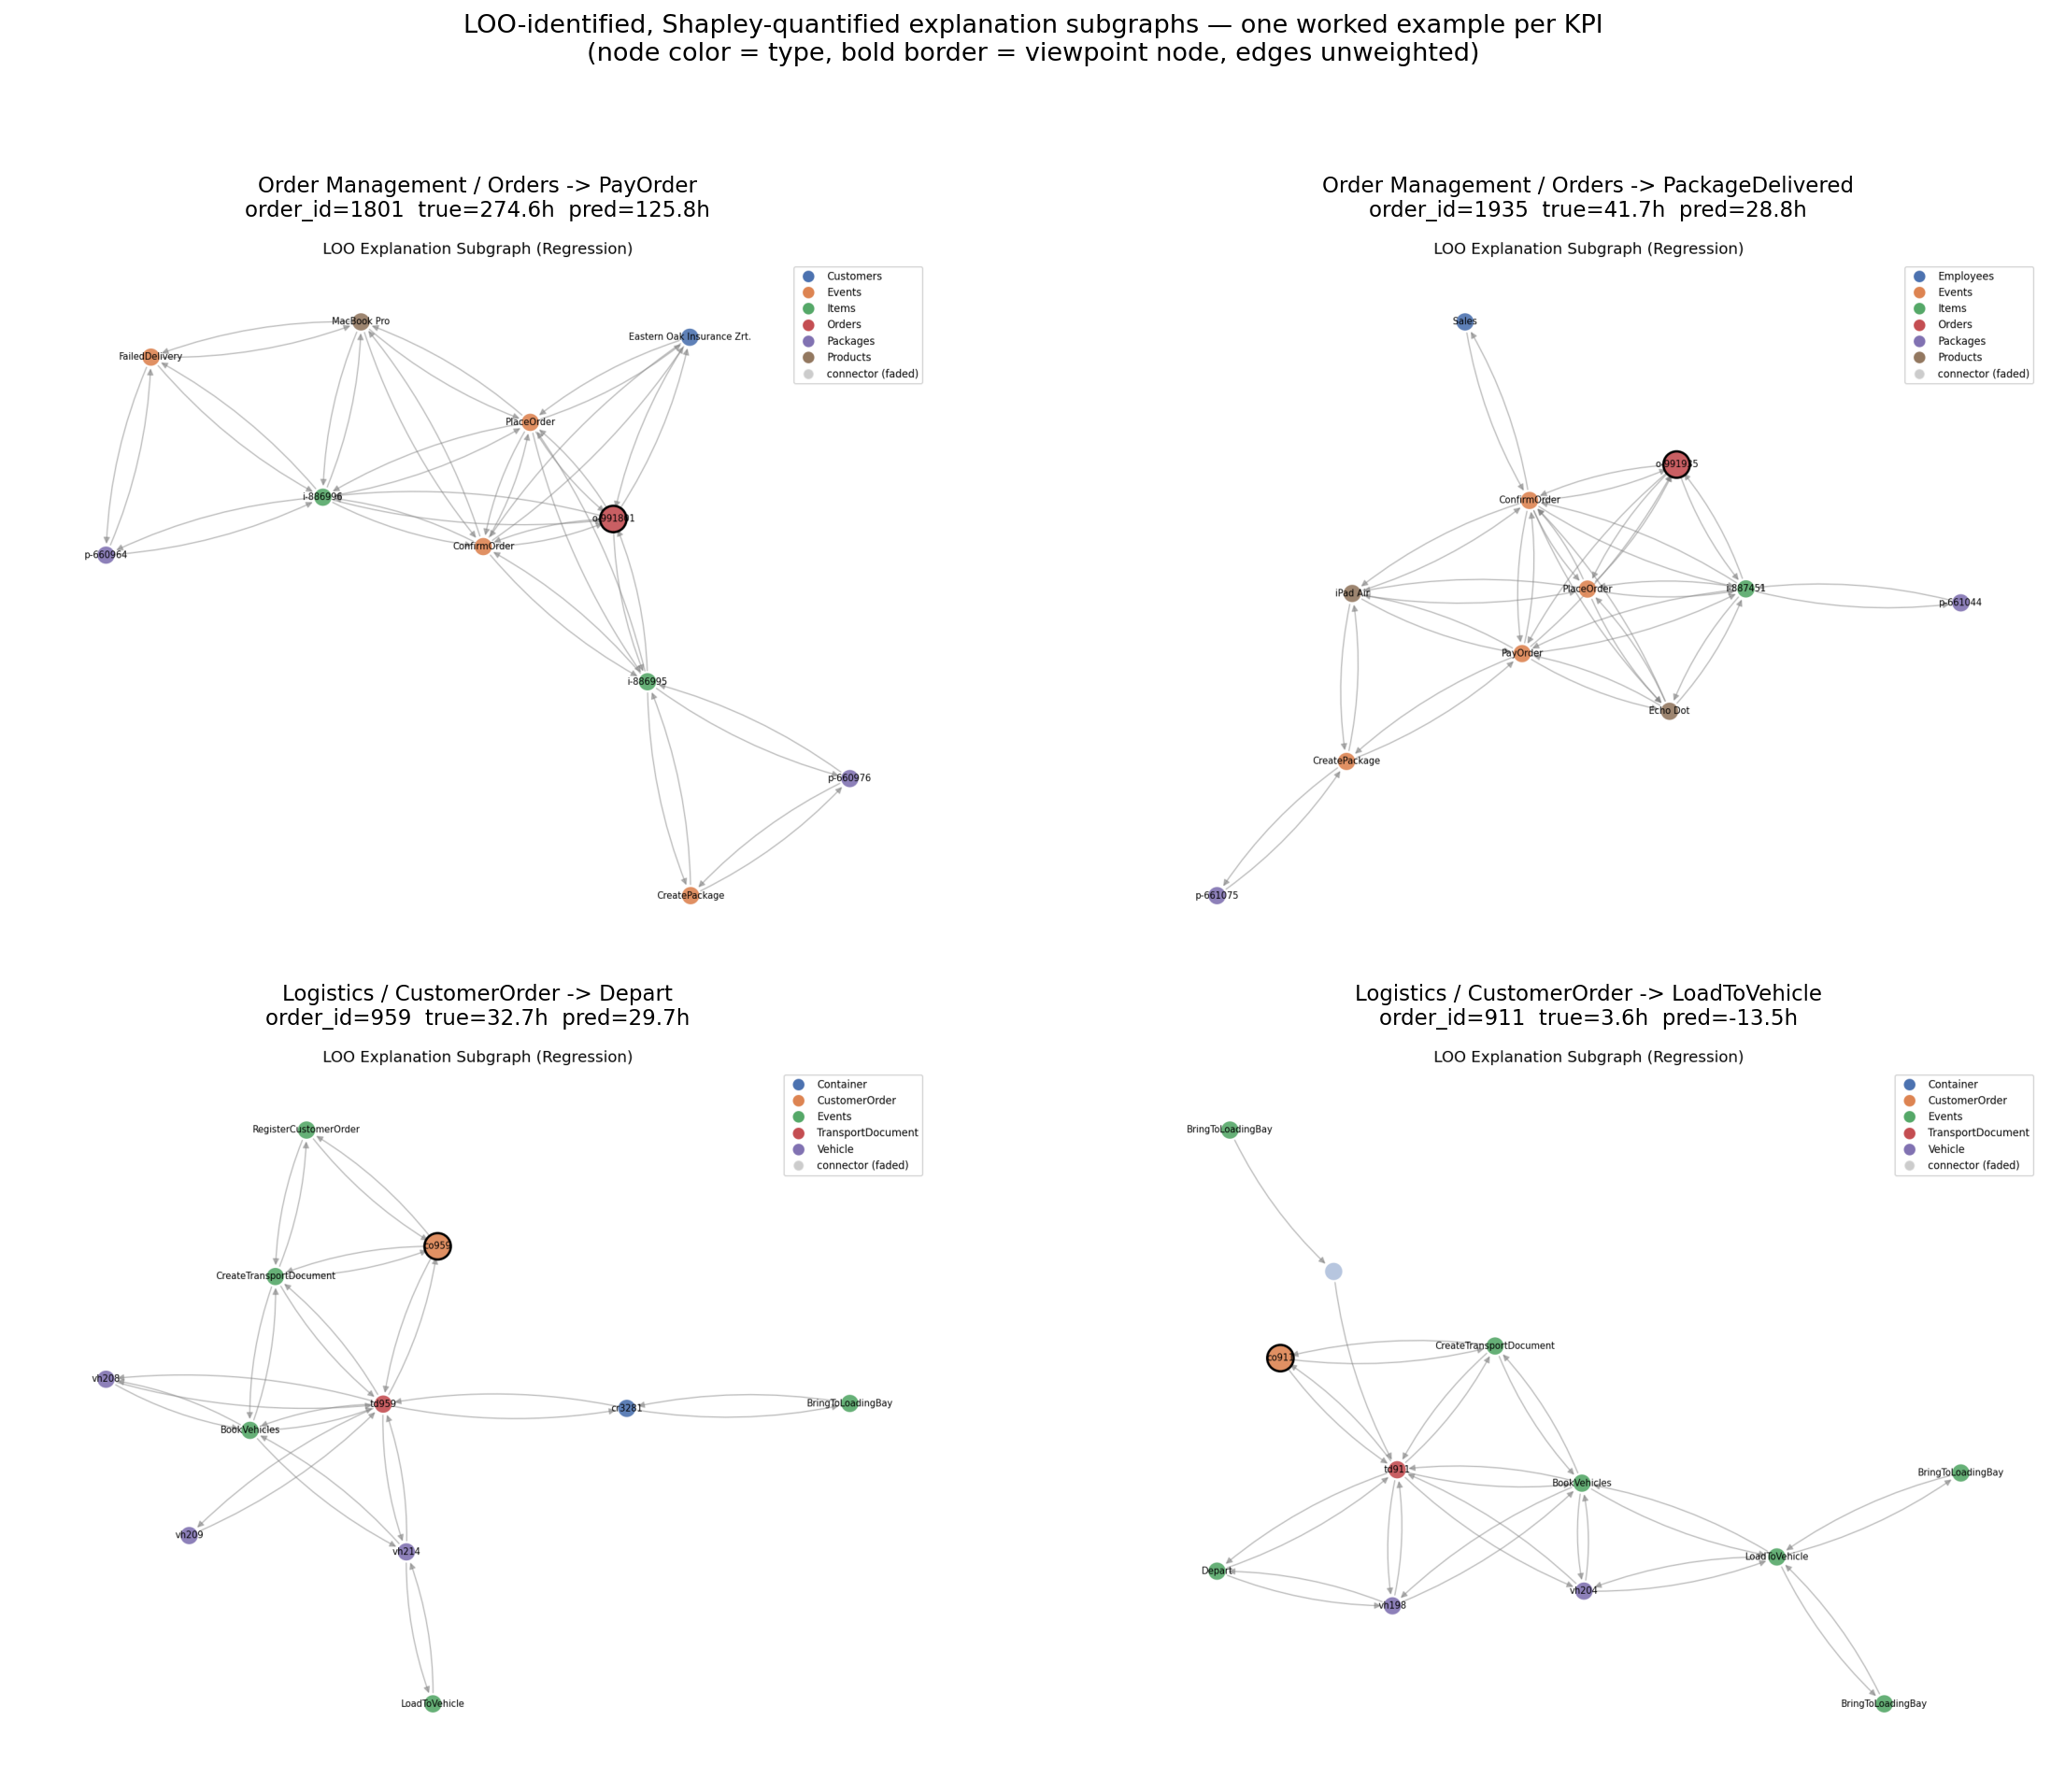
\includegraphics[width=1\textwidth]{figures/single_subgraph.png}
                \caption{Explanation subgraphs created using the identified most important nodes and edges, one worked example per KPI.}
                \label{fig:subgraph}
            \end{figure}
            
            Additionally, the end user is also provided with a visualization of the explanation subgraph created by the explanation. As can be seen in Fig. \ref{fig:subgraph} the subgraph is composed only of the most important elements identified by the explanation and provides another visual way of understanding the most impactful components of the process execution the model looked at when performing its prediction. In other words, the provided subgraph acts as a visual summary of the most impactful components of the input graph.

            \begin{figure}[t!]
                \centering
                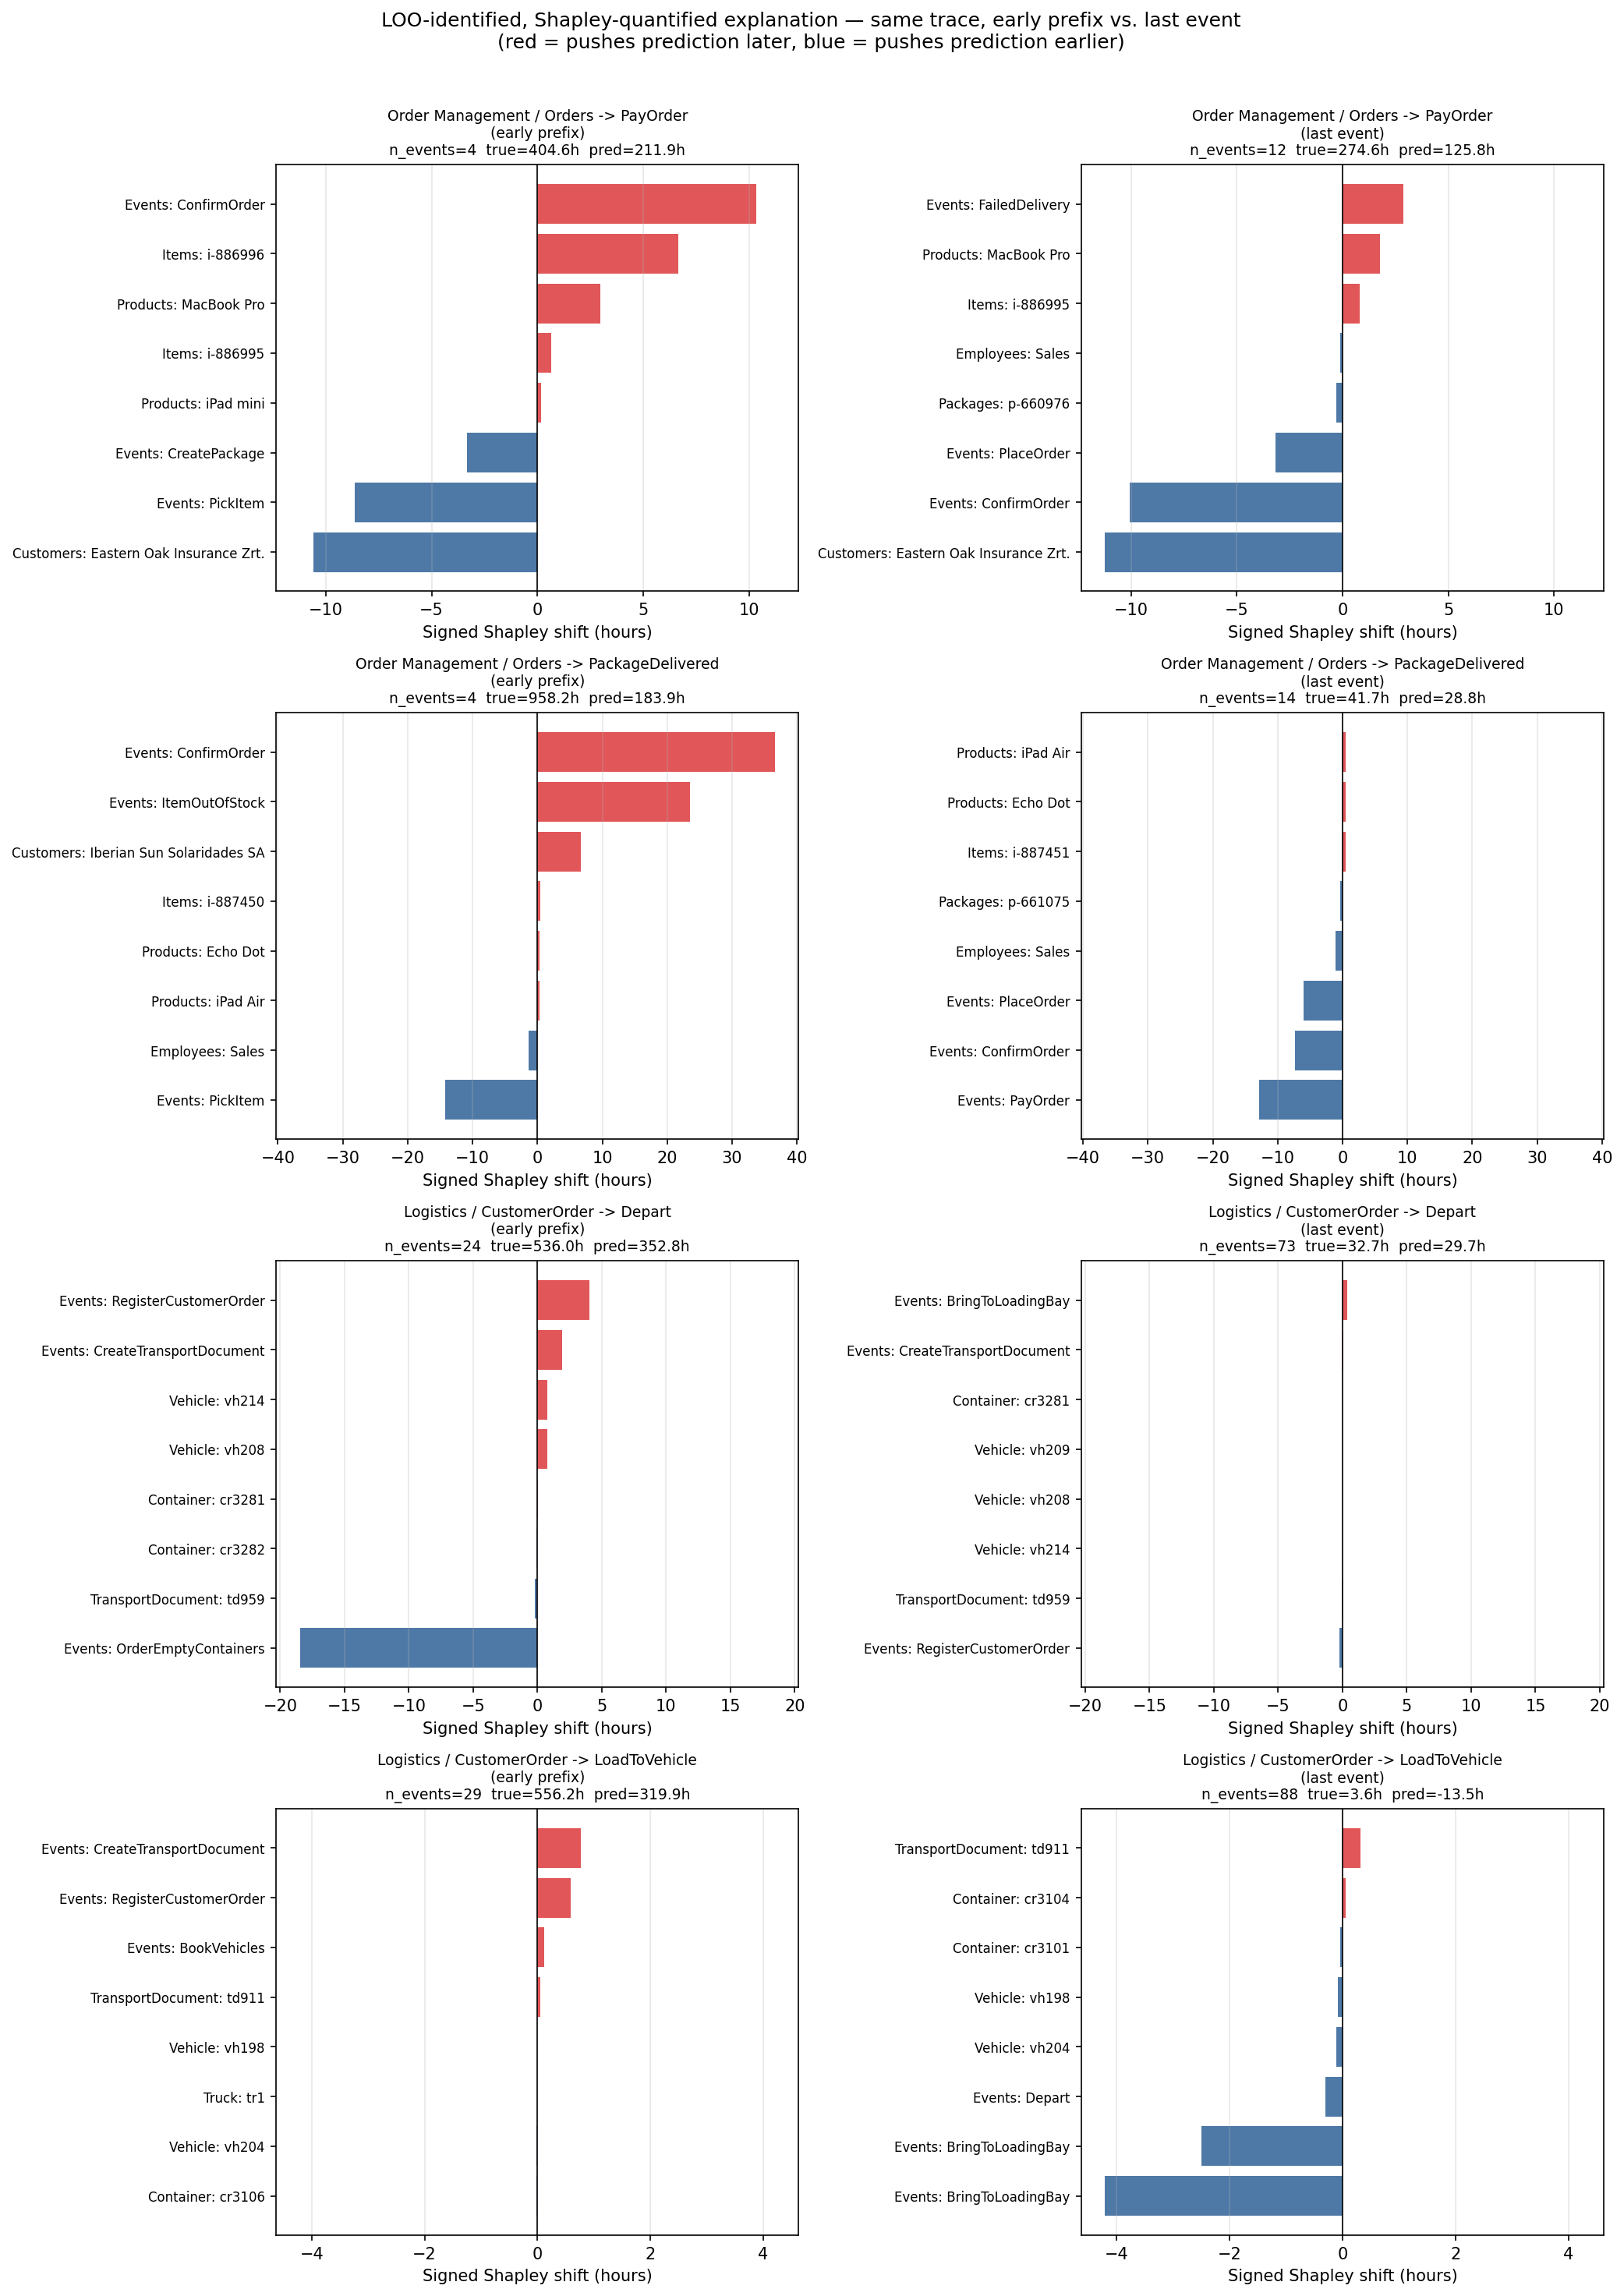
\includegraphics[width=0.85\textwidth]{figures/prefix_evolution.png}
                \caption{Graphs showing the single-trace explanations of node importance generated for an early prefix and the last-event prefix of the same process execution, for each of the four KPIs.}
                \label{fig:prefix_showcase}
            \end{figure}

			Fig. \ref{fig:prefix_showcase} shows that the given explanation can be applied to any prefix in a chosen process execution, giving the stakeholder the ability to view how the importance of elements shifts as the process moves along and more information is provided to the model. As can be seen in the figure, the ranking of important elements changes between the early prefix and the last-event prefix for every KPI shown -- for example, on the Order Management / Orders $\to$ PayOrder KPI, \texttt{ConfirmOrder} is the dominant positive driver on the early prefix but becomes a negative driver by the last event -- highlighting a shift in the model's understanding of the data provided as more information becomes available.
            
            \begin{figure}[t!]
                \centering
                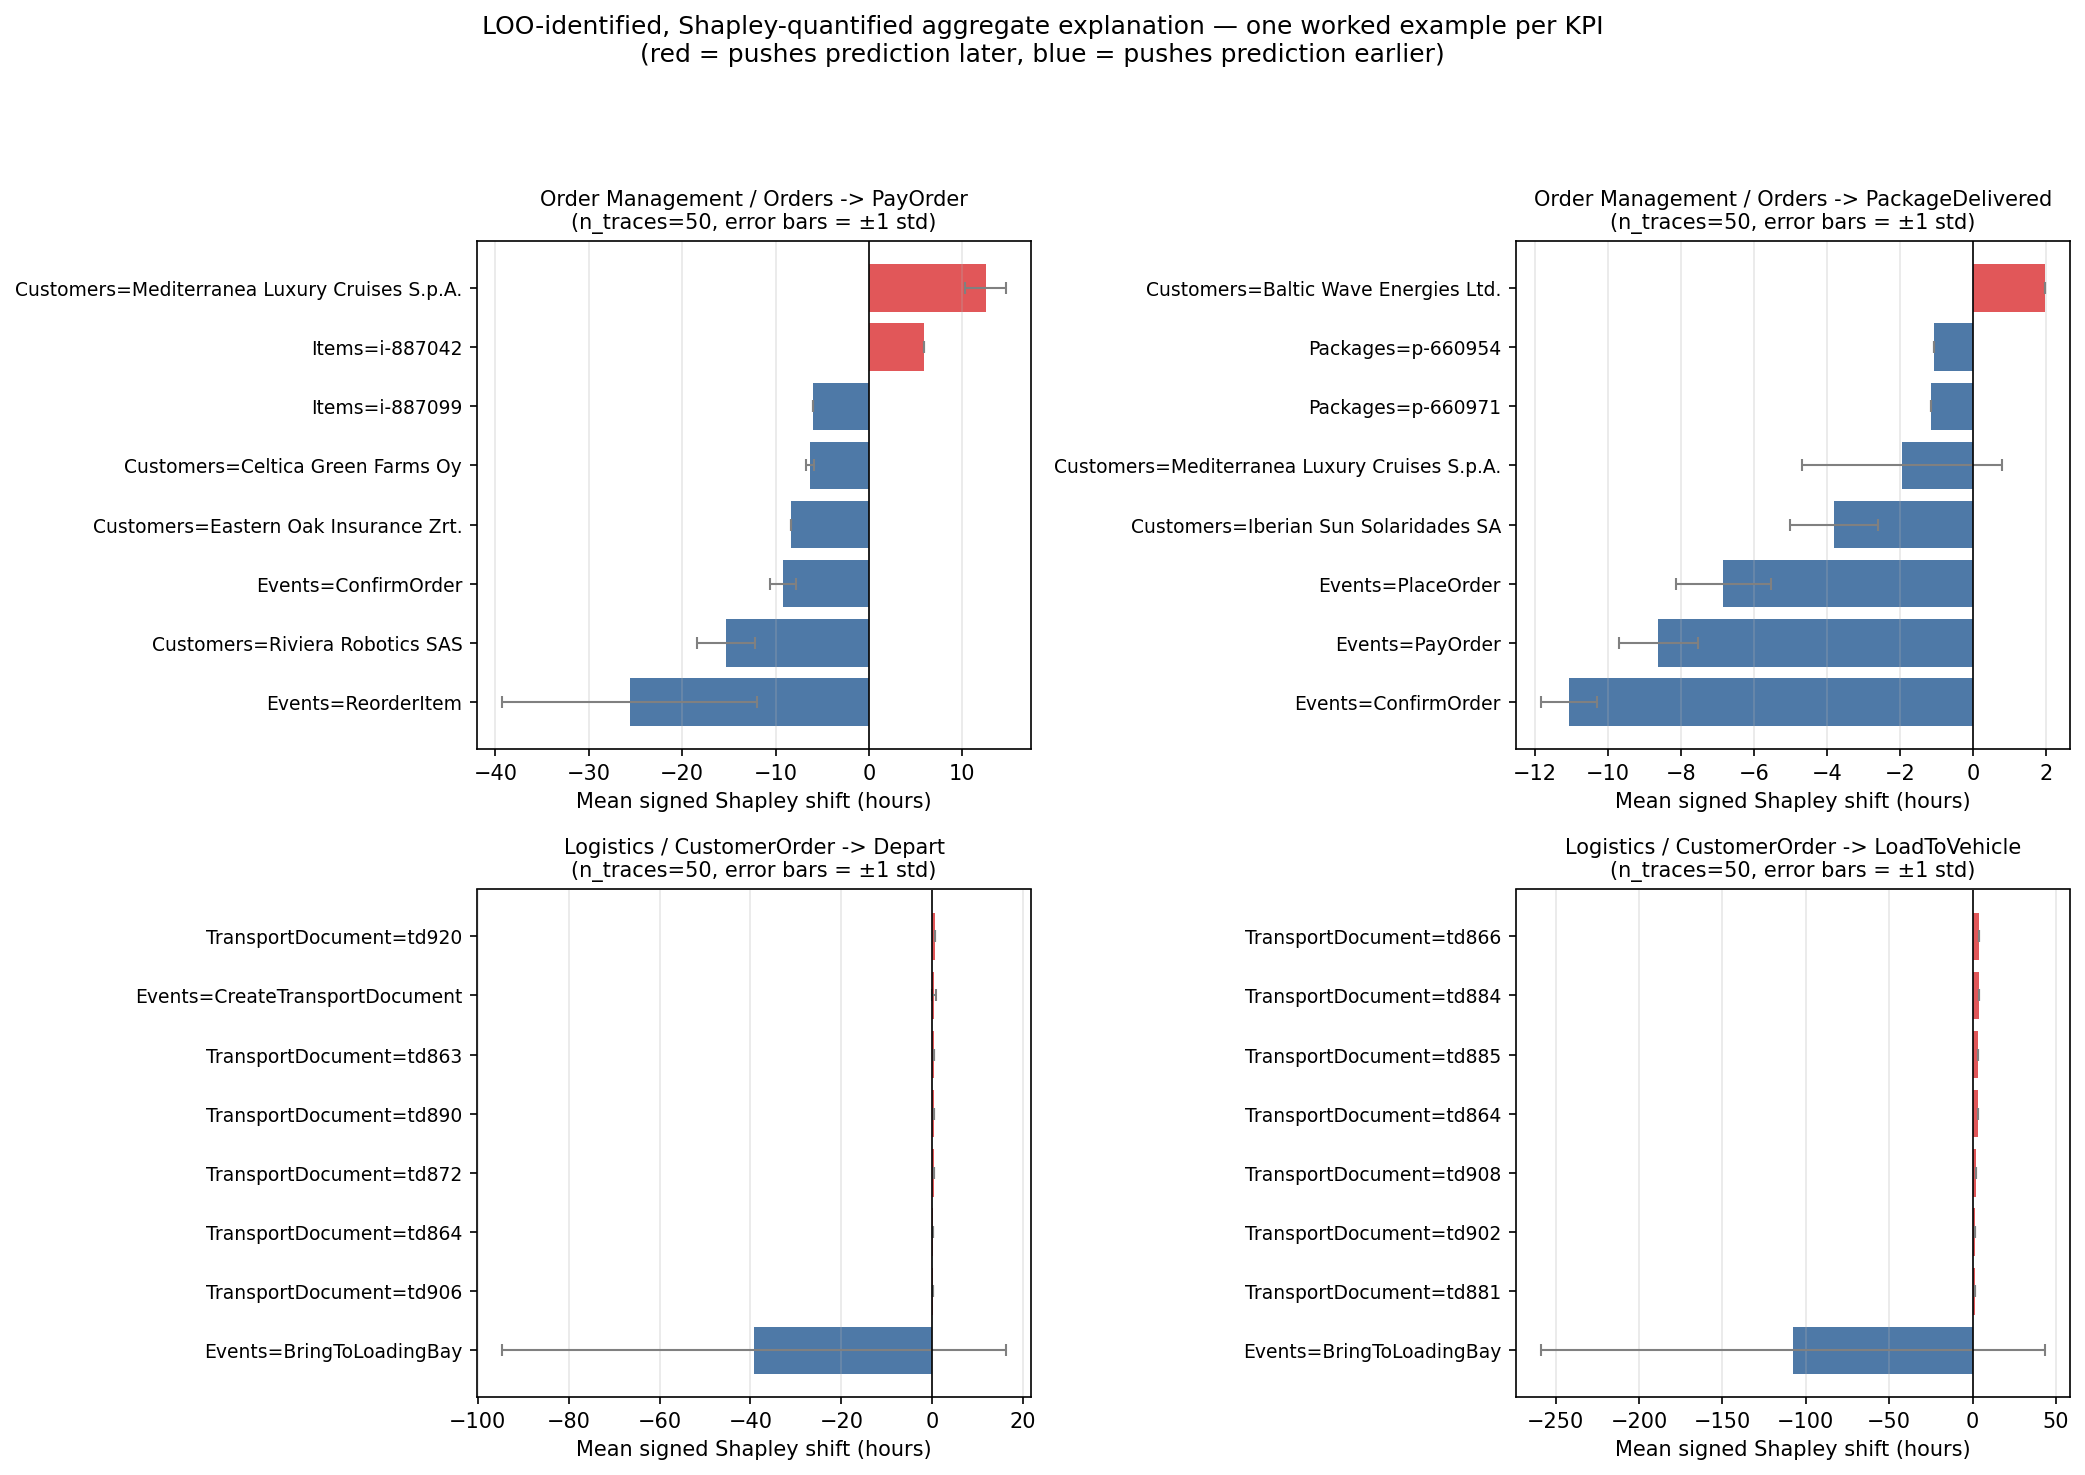
\includegraphics[width=1\textwidth]{figures/loo_shapley_aggregate_showcase.png}
                \caption{Graphs showing the aggregate explanations generated indicating the most important nodes for a collection of 50 traces as well as the impact on the model's prediction.}
                \label{fig:agg_shapley_showcase}
            \end{figure}

            Aside from single traces the stakeholder is also provided with an explanation over an aggregate set of traces. Fig. \ref{fig:agg_shapley_showcase} shows an example of the graphs provided measuring the impact of different node types on the model's prediction. The graphs give a rundown of the most important features of a given type (nodes, edges and their associated feature values) over the chosen universe of prefixes.
			In order to maintain cohesion within the presentation, each graph is designed to mirror its single trace counterpart.

            \subsubsection{Holistic aggregate view}
            \begin{figure}[t!]
                \centering
                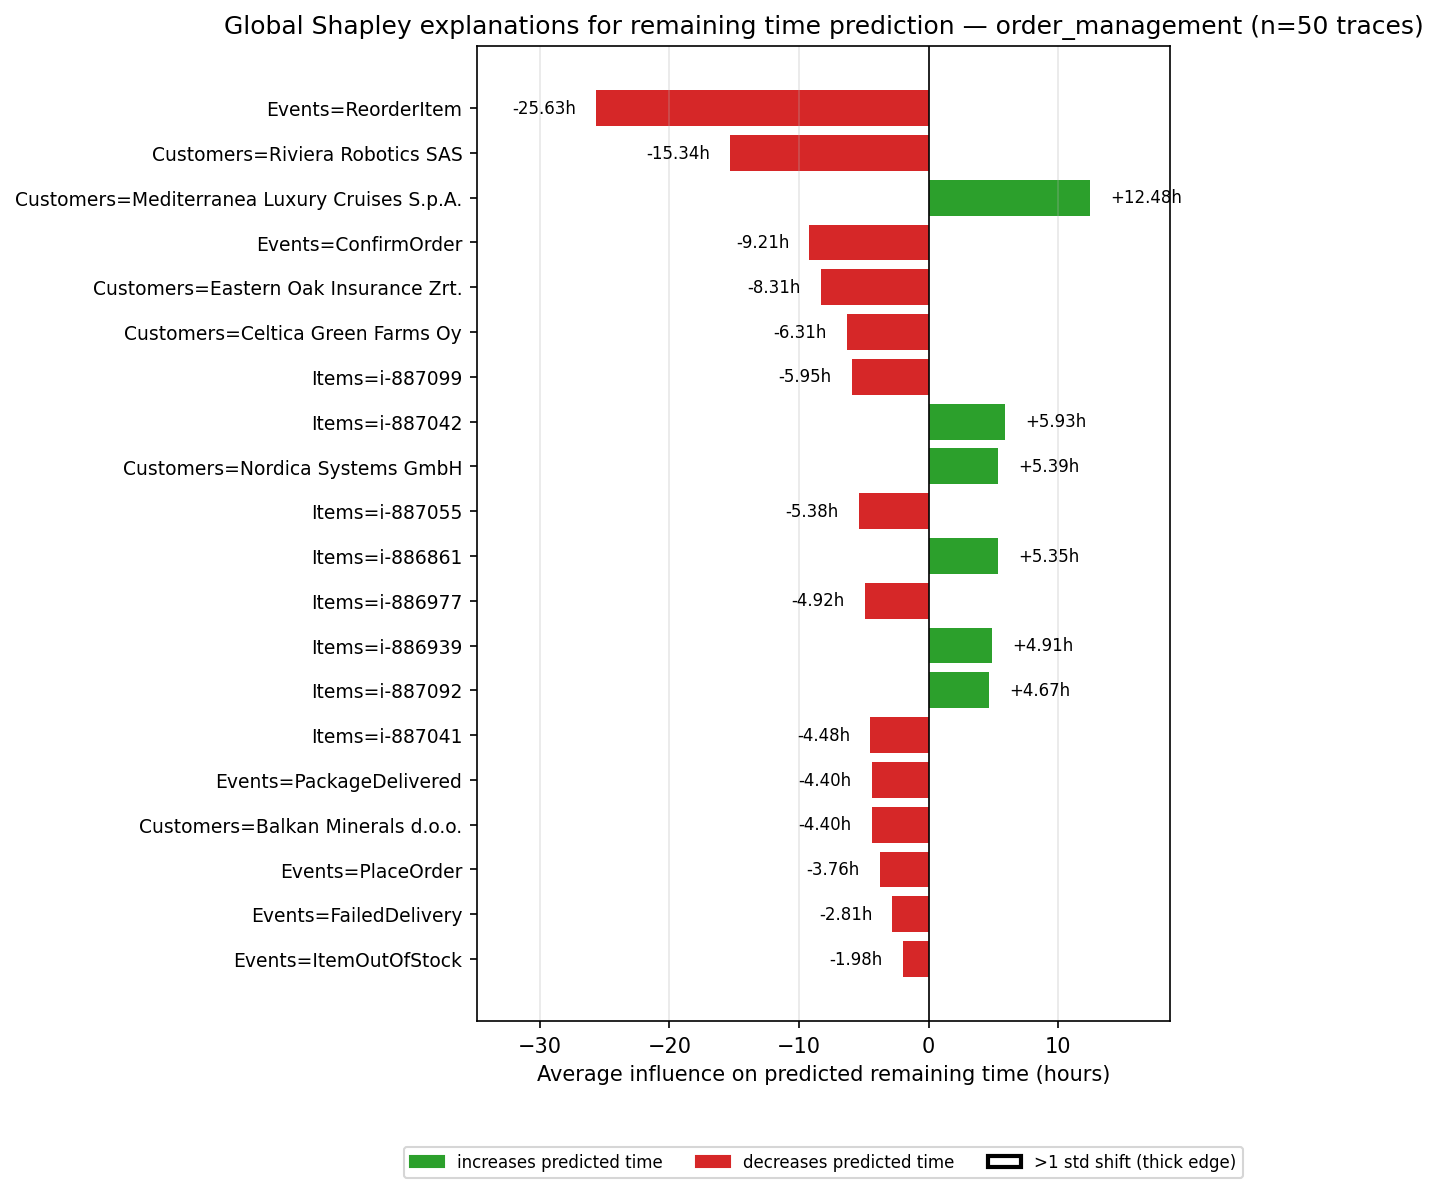
\includegraphics[width=1\textwidth]{figures/aggregate_shapley_global_om_payorder.png}
                \caption{Global LOO+Shapley explanation, ranked across all identified elements, for Order Management / Orders $\to$ PayOrder (50 traces).}
                \label{fig:agg_shapley_global_om_payorder}
            \end{figure}

            \begin{figure}[t!]
                \centering
                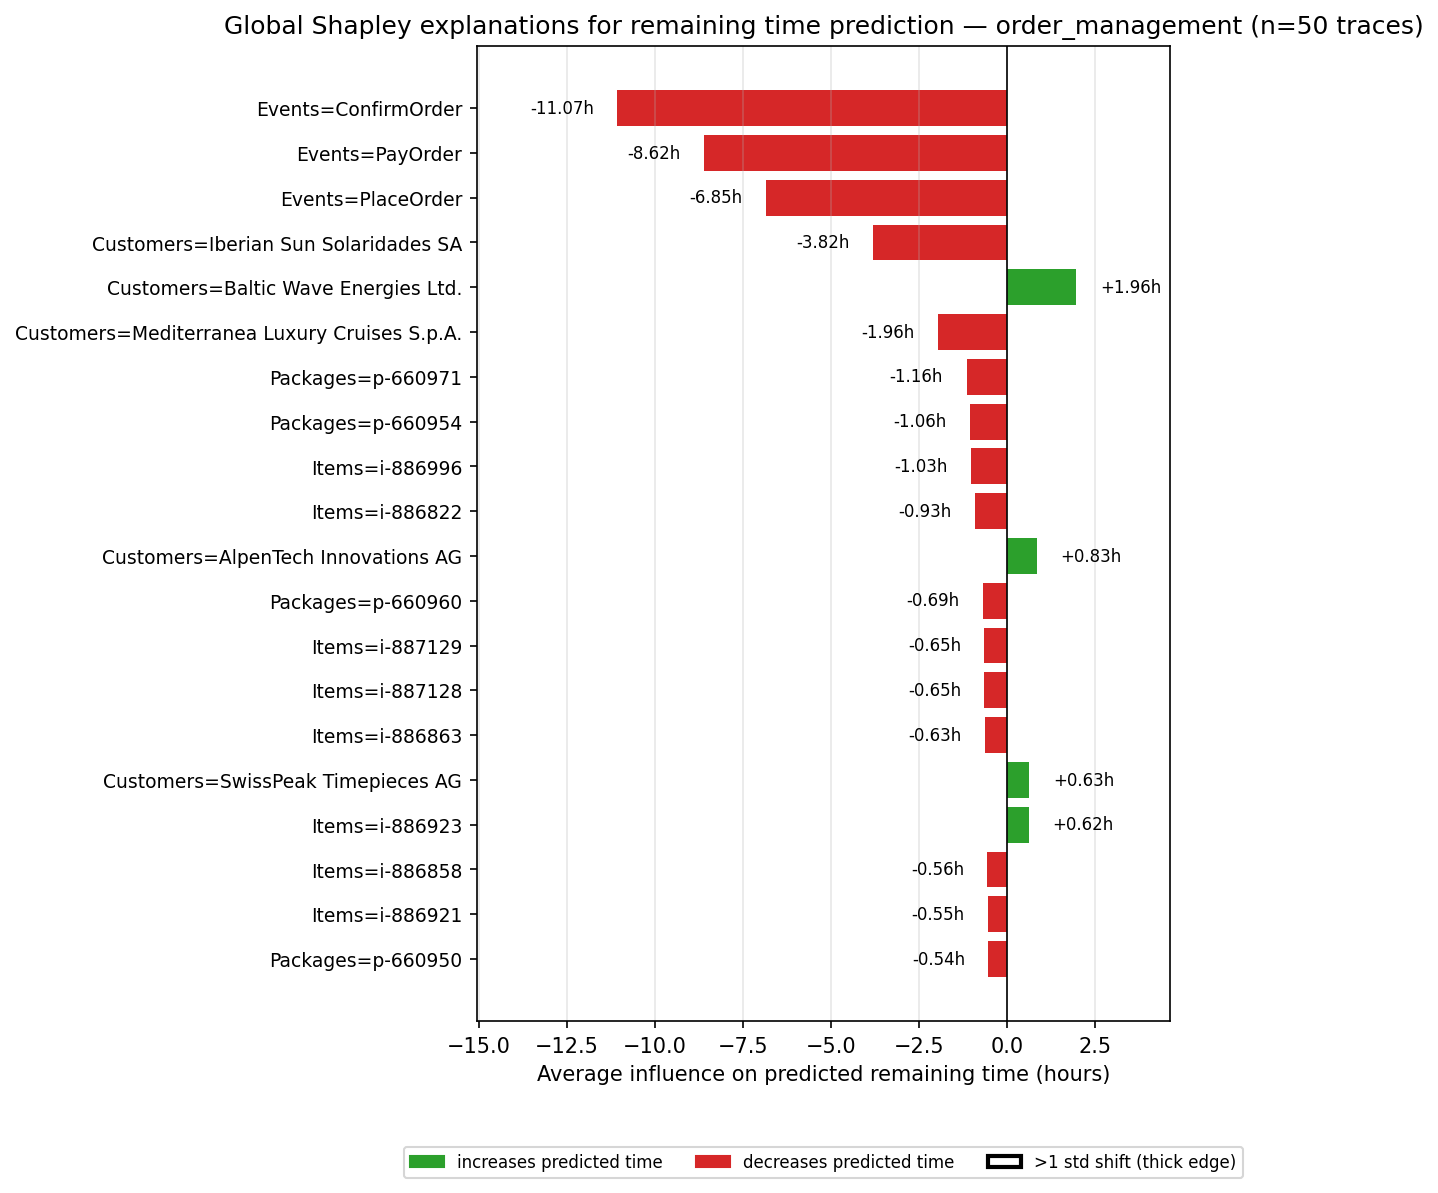
\includegraphics[width=1\textwidth]{figures/aggregate_shapley_global_om_packagedelivered.png}
                \caption{Global LOO+Shapley explanation, ranked across all identified elements, for Order Management / Orders $\to$ PackageDelivered (50 traces).}
                \label{fig:agg_shapley_global_om_packagedelivered}
            \end{figure}

            \begin{figure}[t!]
                \centering
                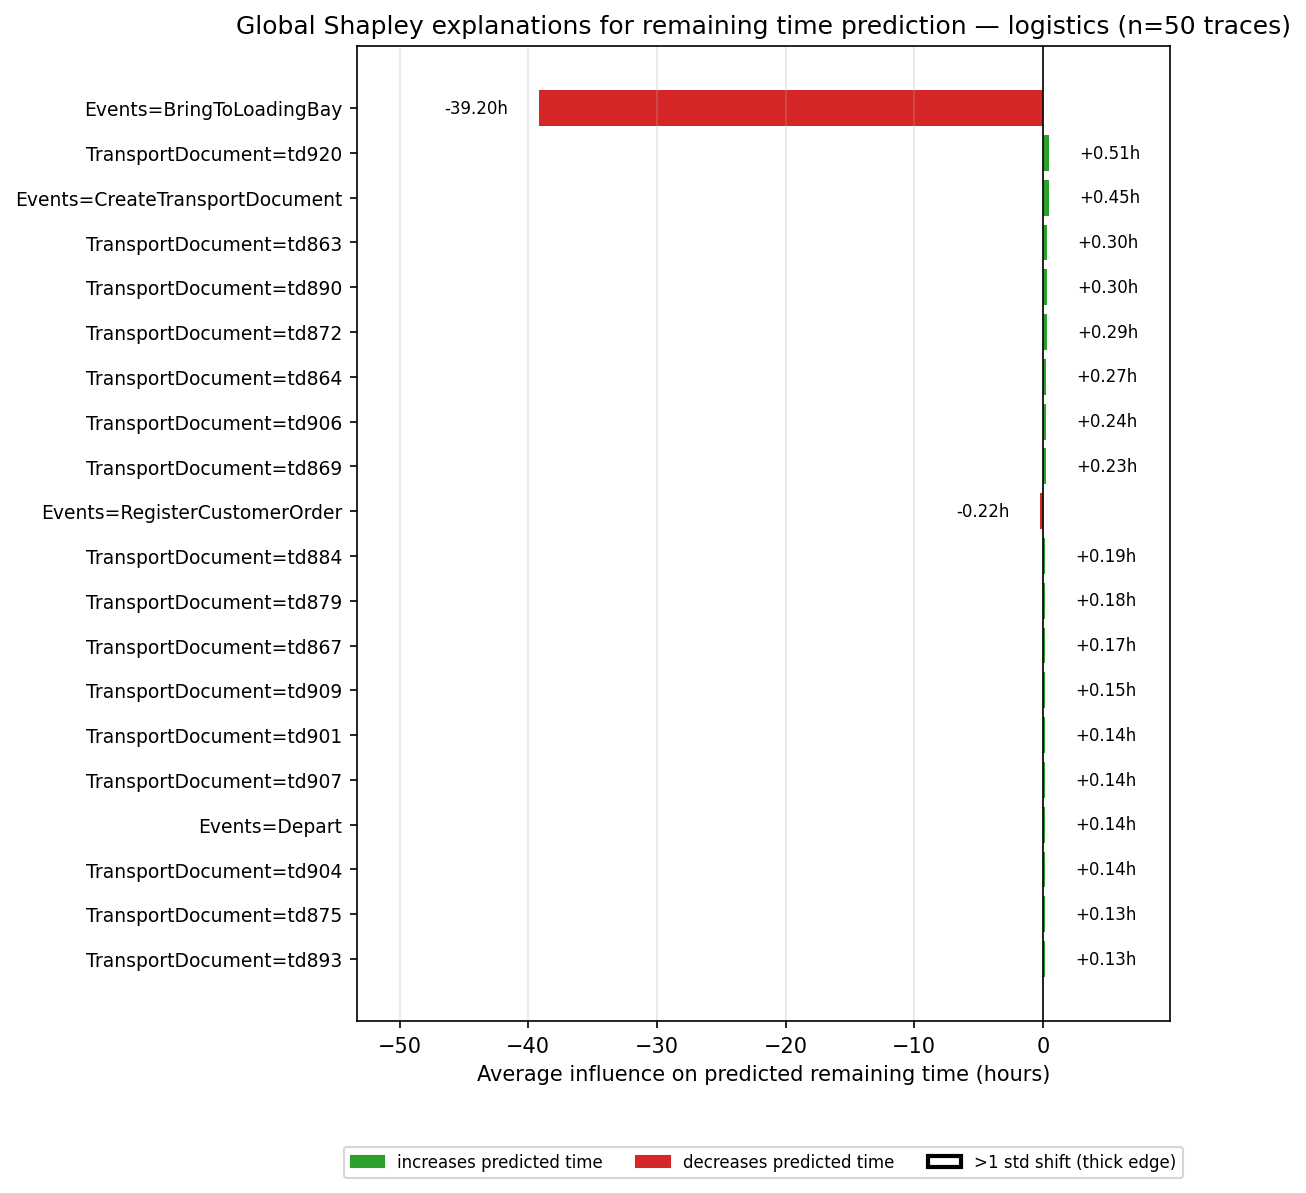
\includegraphics[width=1\textwidth]{figures/aggregate_shapley_global_logistics_depart.png}
                \caption{Global LOO+Shapley explanation, ranked across all identified elements, for Logistics / CustomerOrder $\to$ Depart (50 traces).}
                \label{fig:agg_shapley_global_logistics_depart}
            \end{figure}

            \begin{figure}[t!]
                \centering
                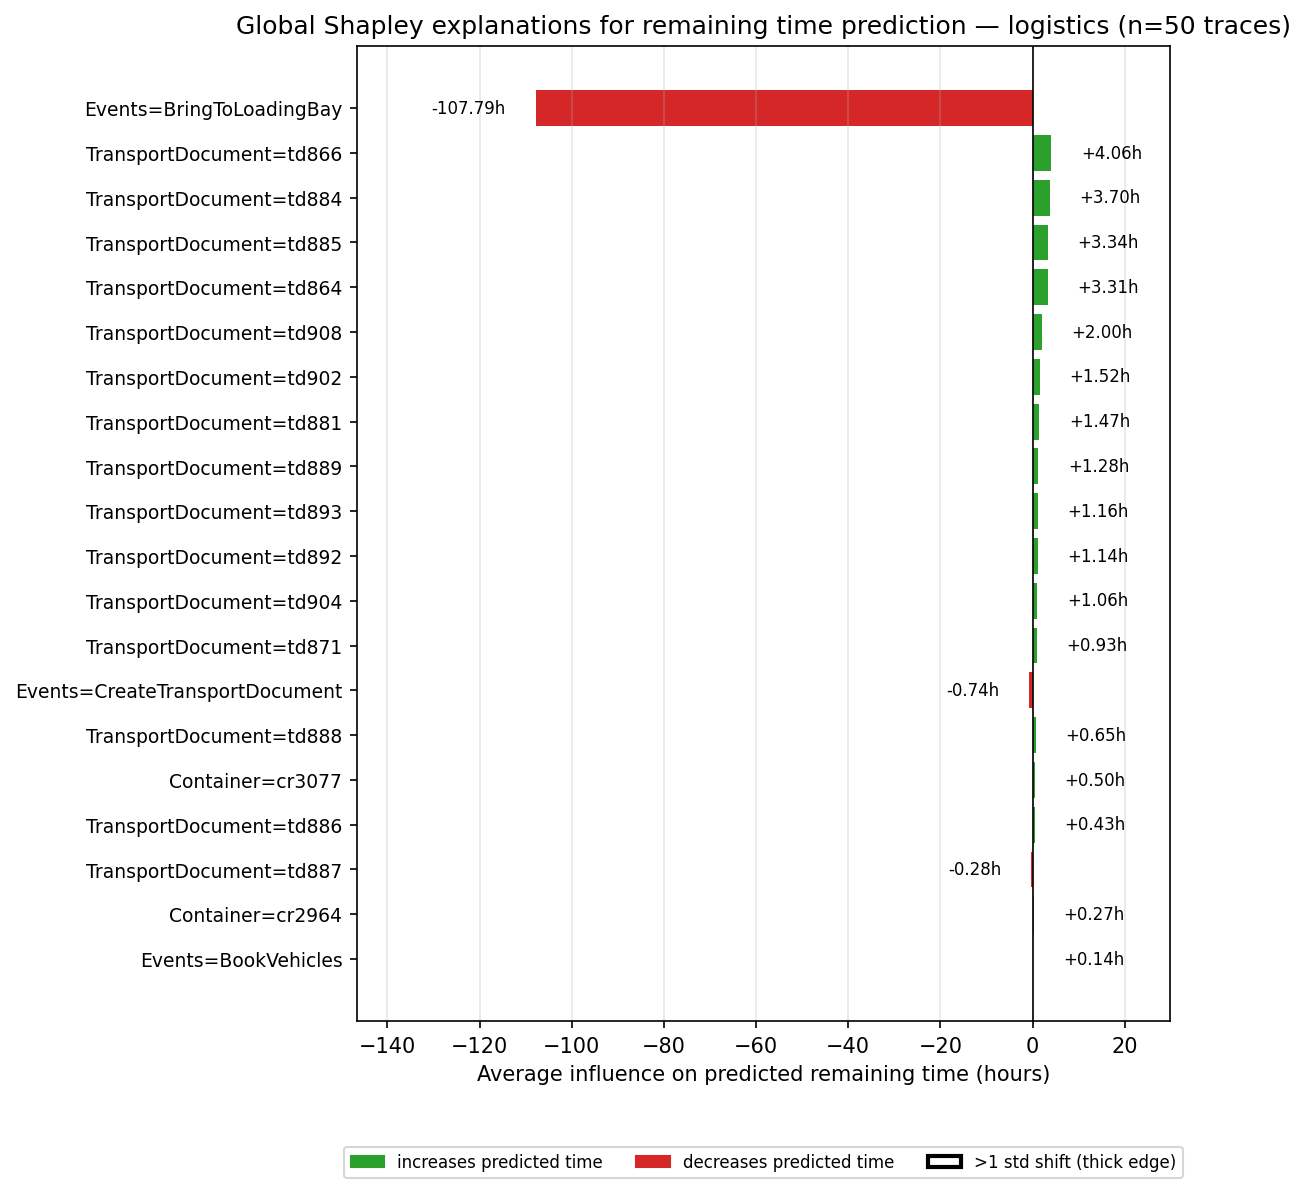
\includegraphics[width=1\textwidth]{figures/aggregate_shapley_global_logistics_loadtovehicle.png}
                \caption{Global LOO+Shapley explanation, ranked across all identified elements, for Logistics / CustomerOrder $\to$ LoadToVehicle (50 traces).}
                \label{fig:agg_shapley_global_logistics_loadtovehicle}
            \end{figure}

            The graphs shown so far in this section describe the \emph{quality} of the explanations -- how faithful they are (Fig. \ref{fig:loo_comparison}), how consistent LOO is with full Shapley Values (Fig. \ref{fig:loo_shapley_comp}) -- or, in Fig. \ref{fig:agg_shapley_showcase}'s case, a compact per-KPI summary limited to a handful of elements. None of them give a single, holistic view of what the framework identifies as important across the dataset as a whole. Figs. \ref{fig:agg_shapley_global_om_payorder}-\ref{fig:agg_shapley_global_logistics_loadtovehicle} close that gap: each is a single ranked list, pooled across the same 50 traces per KPI used elsewhere in this section, showing every node identity (event type, customer, item, package, transport document, etc.) whose presence shifted the model's prediction, signed and ranked by its average impact. Rather than illustrating one trace or comparing two methods, these graphs give the stakeholder a genuine ``helicopter view'' of the model's behavior as a whole: which recurring elements of the process consistently push predictions earlier or later, independent of any single example.

        \subsection{Gradient/feature-based explanation}
            \begin{figure}[t!]
                \centering
                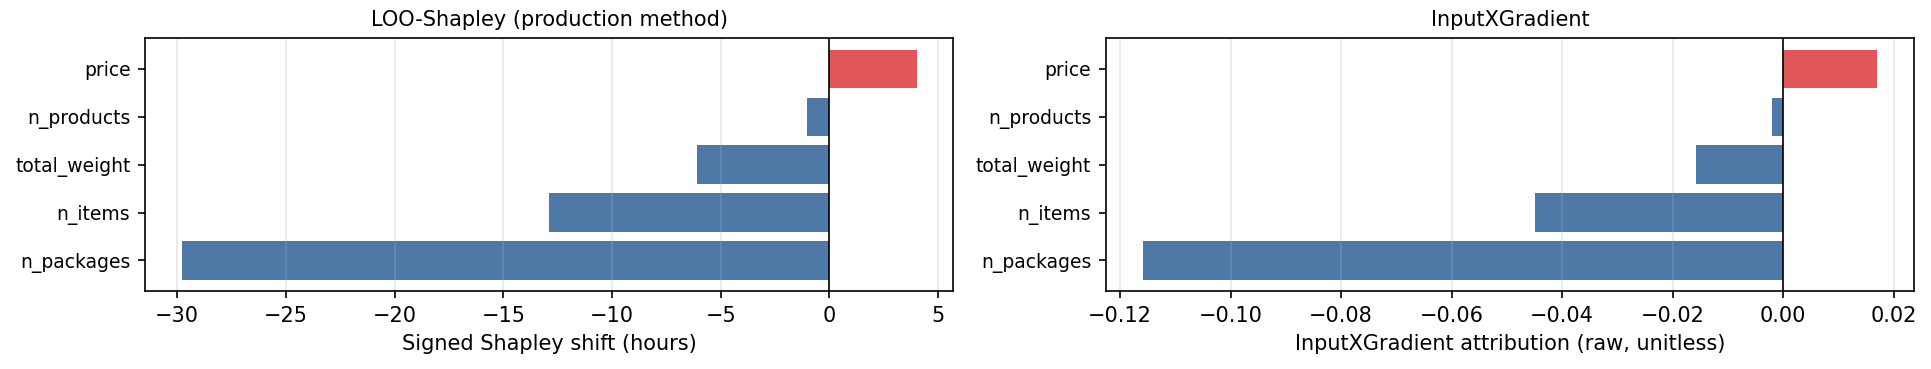
\includegraphics[width=1\textwidth]{figures/gradient_shapley_comparison_inputxgradient.png}
                \caption{Graphs showing the single-trace explanation provided for feature importance on the Order node using the Gradient $\cdot$ Input method for identification and the LOO-Shapley method for quantifying the feature's impact on the prediction.}
                \label{fig:input_gradient}
            \end{figure}

            \begin{figure}[t!]
                \centering
                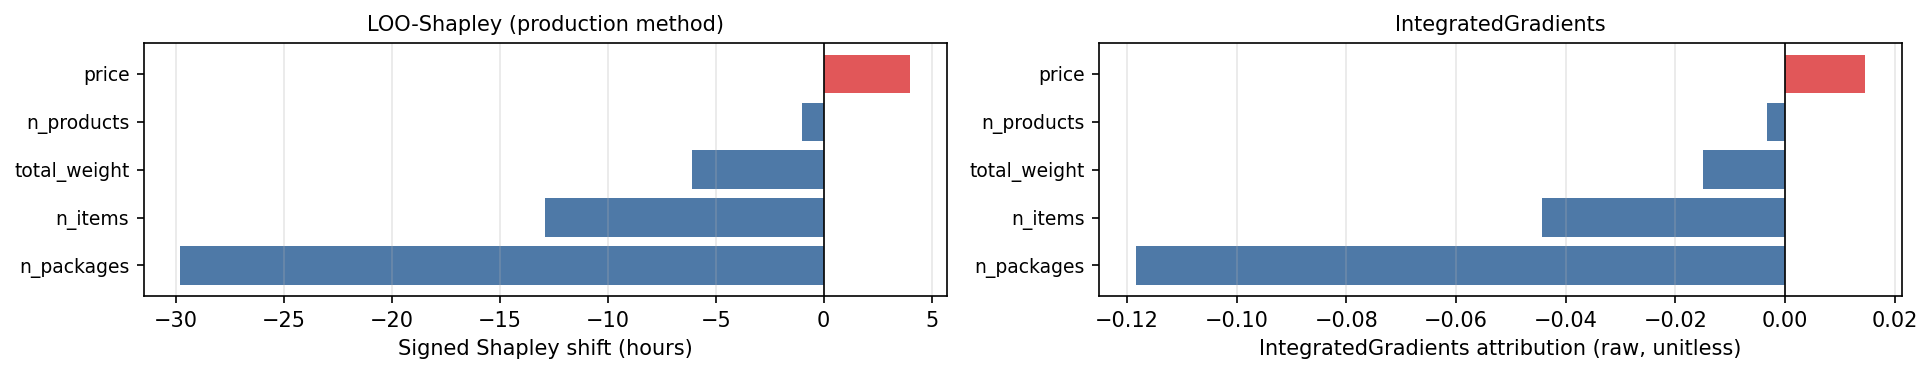
\includegraphics[width=1\textwidth]{figures/gradient_shapley_comparison_integratedgradients.png}
                \caption{Graphs showing the single-trace explanation provided for feature importance on the Order node using the Integrated Gradients method for identification and the LOO-Shapley method for quantifying the feature's impact on the prediction.}
                \label{fig:integ_gradients}
            \end{figure}
            
            While node and edge importance are calculated exclusively through the use of the perturbation-based method their associated feature values follow a different methodology. Fig. \ref{fig:input_gradient} and Fig. \ref{fig:integ_gradients} show the ranking of feature importance for the feature values present in a given trace for the Orders node. The values presented in the right side graph of Fig. \ref{fig:input_gradient} refer to the attribution values calculated through the chosen gradient-based explanation method, in this case Gradient $\cdot$ Input. In order to present this value in a quantifiable way the stakeholder is also shown a graph such as the one in the left side. This graph provides the physical magnitude of the impact for each of the identified feature values from the first analysis. The graph follows the same design as the graphs shown for the other elements of the input graph in order to maintain cohesion in the presentation. Fig. \ref{fig:integ_gradients} showcases that the methodology allows the stakeholder to choose their desired feature attribution method if they wished to compare the rankings provided by each one.

            \begin{figure}[t!]
                \centering
                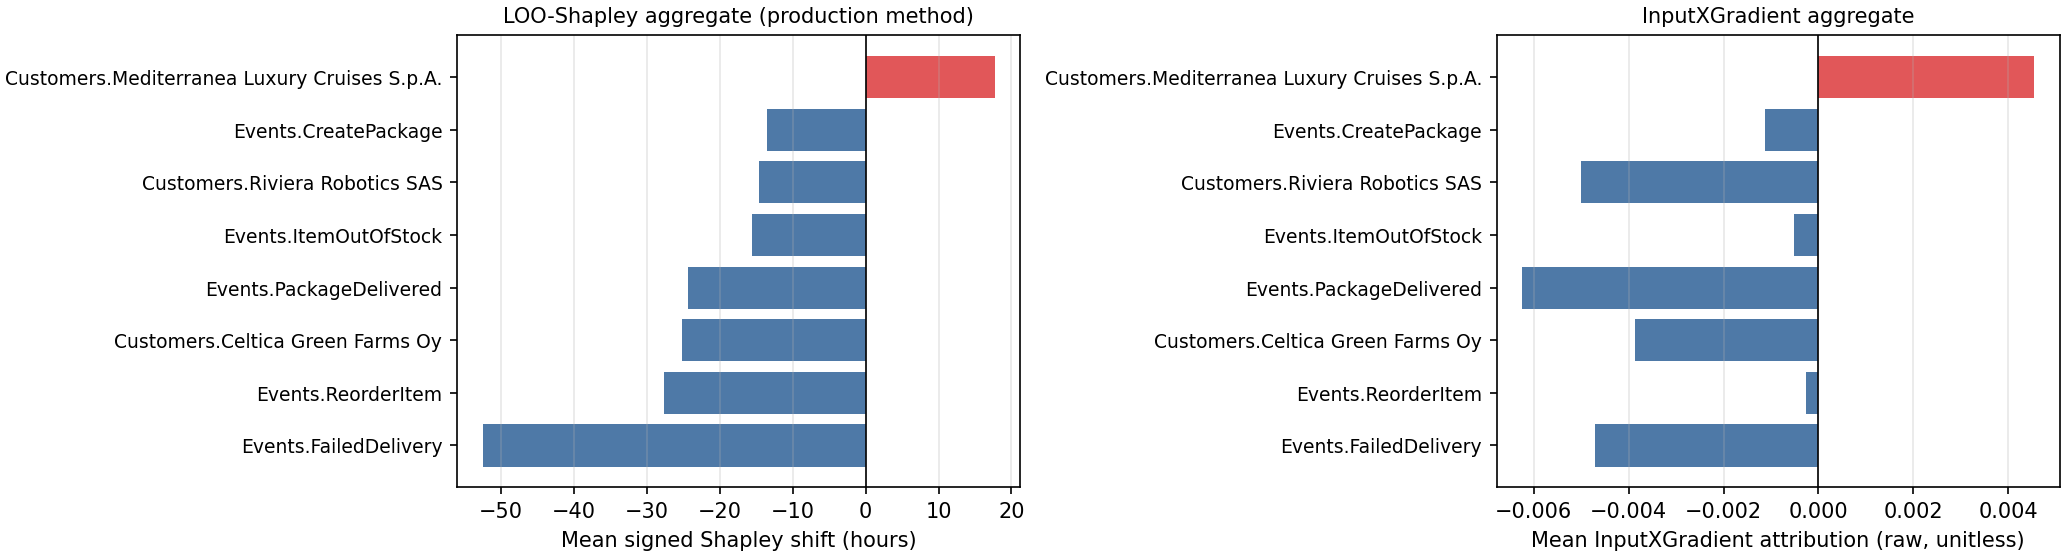
\includegraphics[width=1\textwidth]{figures/feature_attribution_aggregate_shapley_comparison_inputxgradient.png}
                \caption{Graphs showing the aggregate explanation provided for feature importance of the nodes in the chosen traces using the Gradients $\cdot$ Input method for identification and the LOO-Shapley method for quantifying the feature's impact on the prediction.}
                \label{fig:agg_input_gradients}
            \end{figure}

            \begin{figure}[t!]
                \centering
                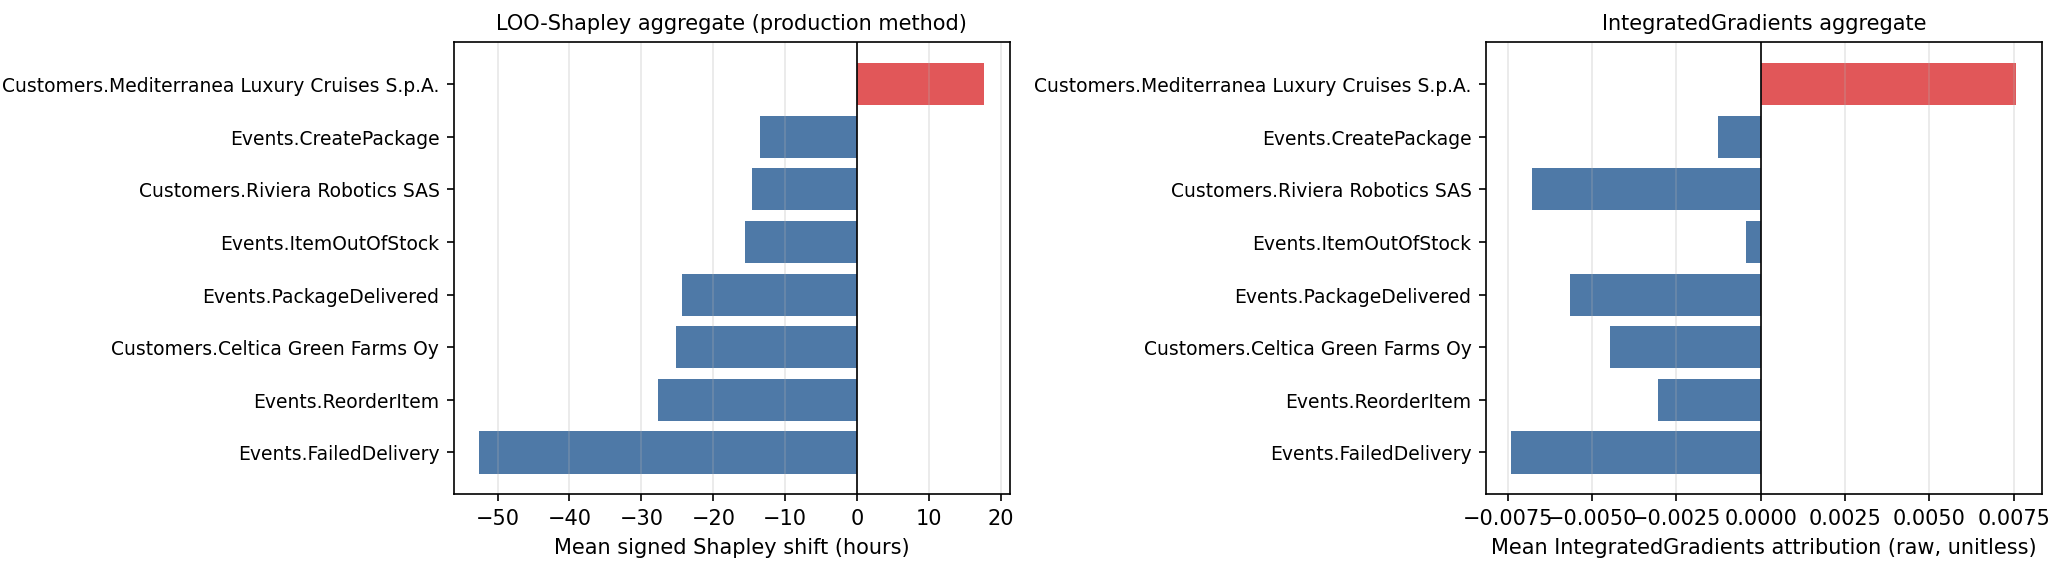
\includegraphics[width=1\textwidth]{figures/feature_attribution_aggregate_shapley_comparison_integratedgradients.png}
                \caption{Graphs showing the aggregate explanation provided for feature importance of the nodes in the chosen traces using the Integrated Gradients method for identification and the LOO-Shapley method for quantifying the feature's impact on the prediction.}
                \label{fig:agg_integ_gradients}
            \end{figure}
            
            In the same vein as the perturbation-based explanation, this method can also be applied to a collection of prefixes in an aggregate analysis. Fig. \ref{fig:agg_input_gradients} and Fig. \ref{fig:agg_integ_gradients} show the resulting graphs. Following the pattern shown for the first explanation, the stakeholder is presented with a graph that identifies the most impactful features of the nodes over the entire prefix set as well as the average impact their presence has on the model's predicted output. Same as with the single-trace analysis, the stakeholder is able to choose which gradient method they prefer to use for the explanation, allowing them to compare the results of each methodology.

        \subsection{Counterfactual explanation}
        \begin{figure}[t!]
                \centering
                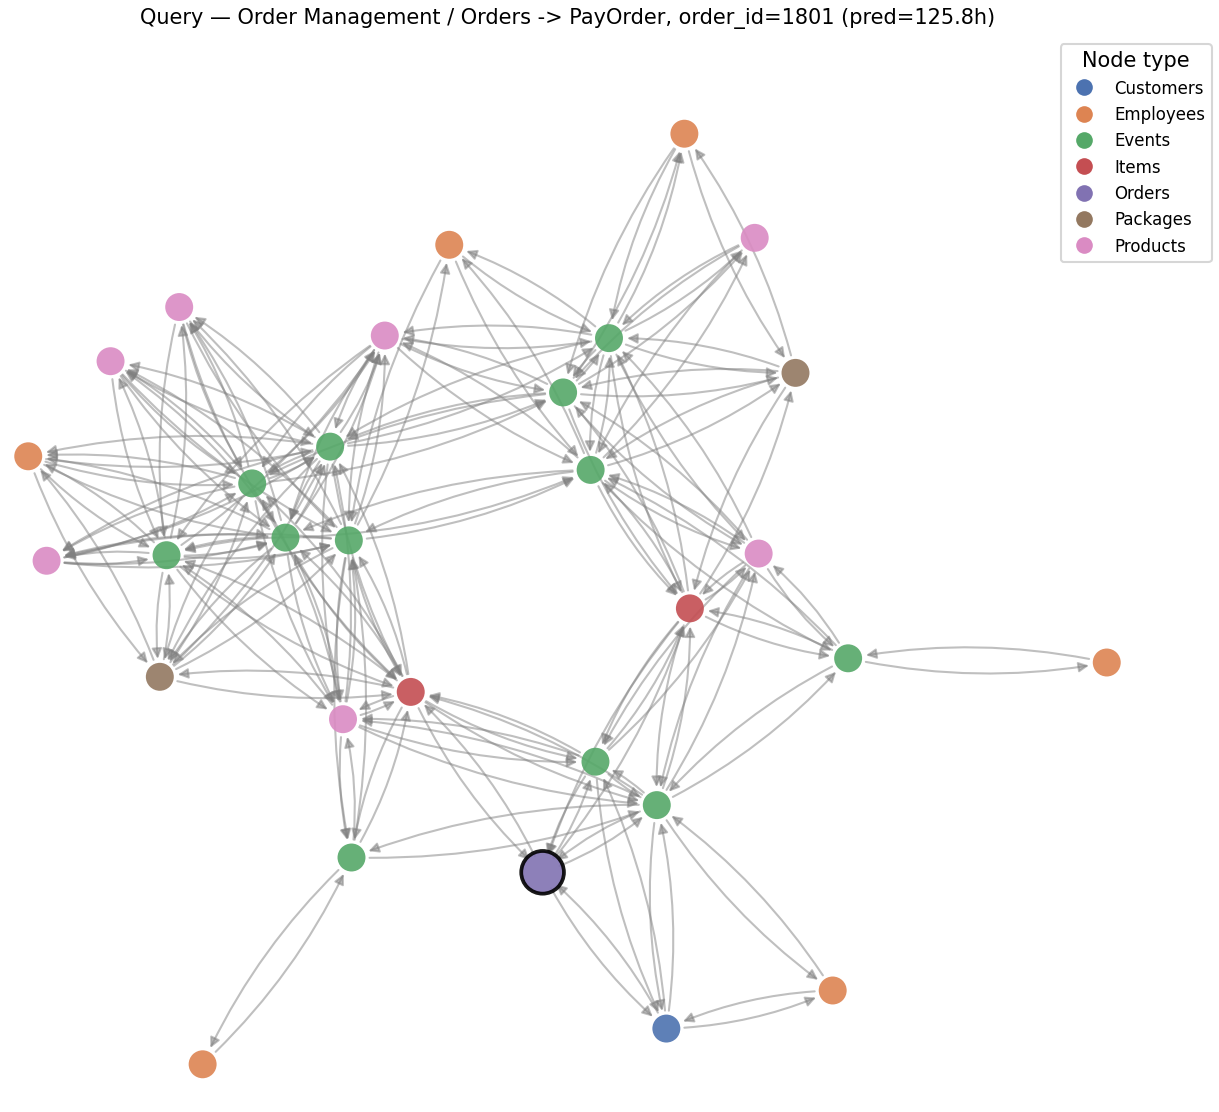
\includegraphics[width=1\textwidth]{figures/cf_showcase_query_graph.png}
                \caption{Graph representation of the user's selected graph for counterfactual explanation.}
                \label{fig:cf_query_graph}
            \end{figure}

        \begin{figure}[t!]
            \centering
            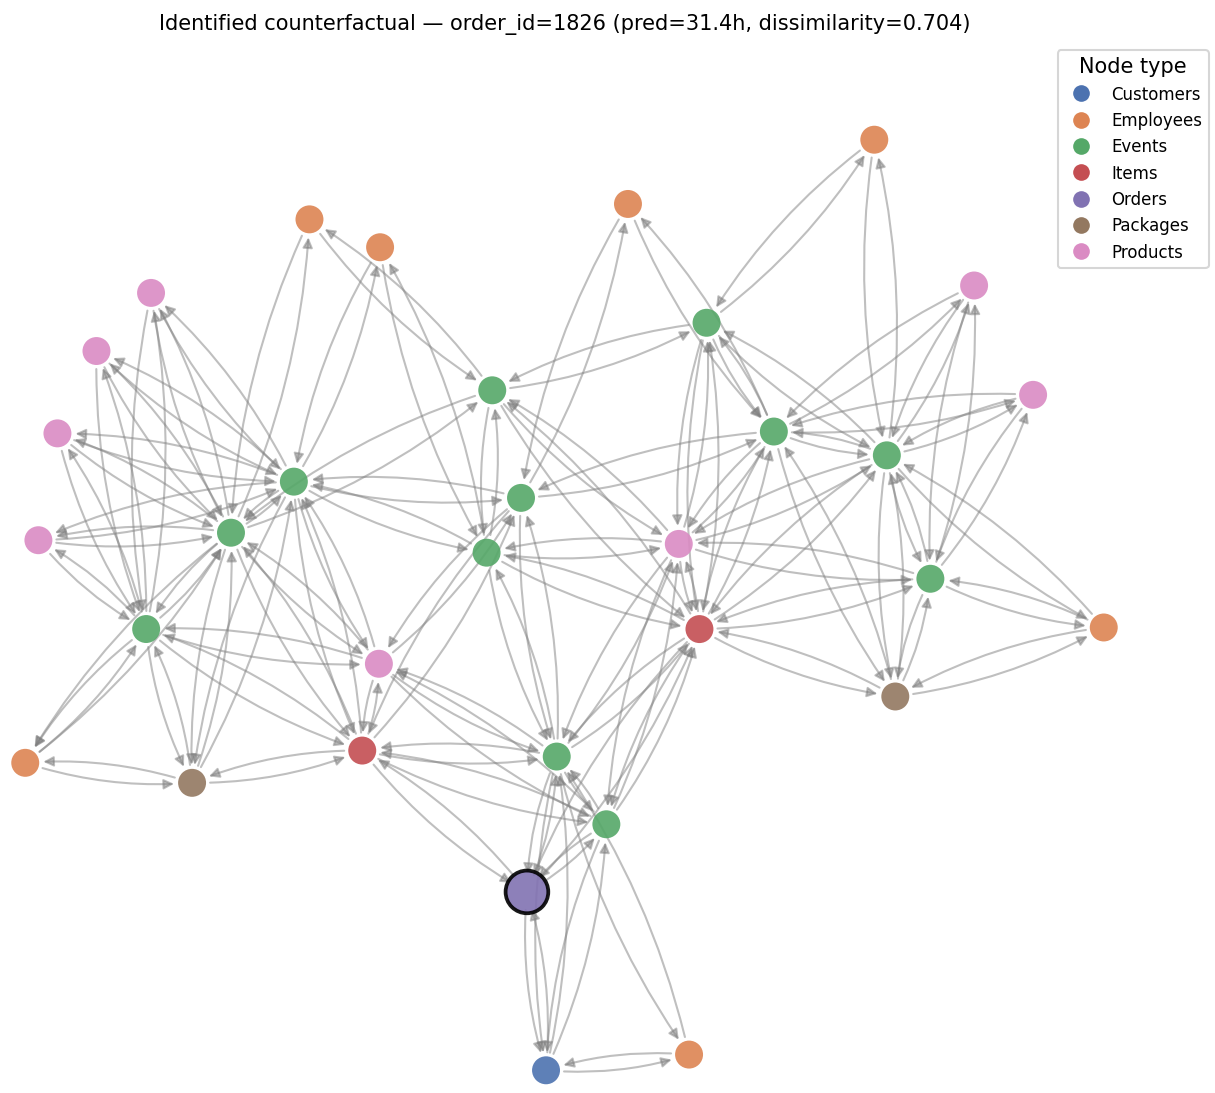
\includegraphics[width=1\textwidth]{figures/cf_showcase_counterfactual_graph.png}
            \caption{Graph representation of the counterfactual graph identified for counterfactual explanation.}
            \label{fig:cf_graph}
        \end{figure}

        \begin{figure}[t!]
            \centering
            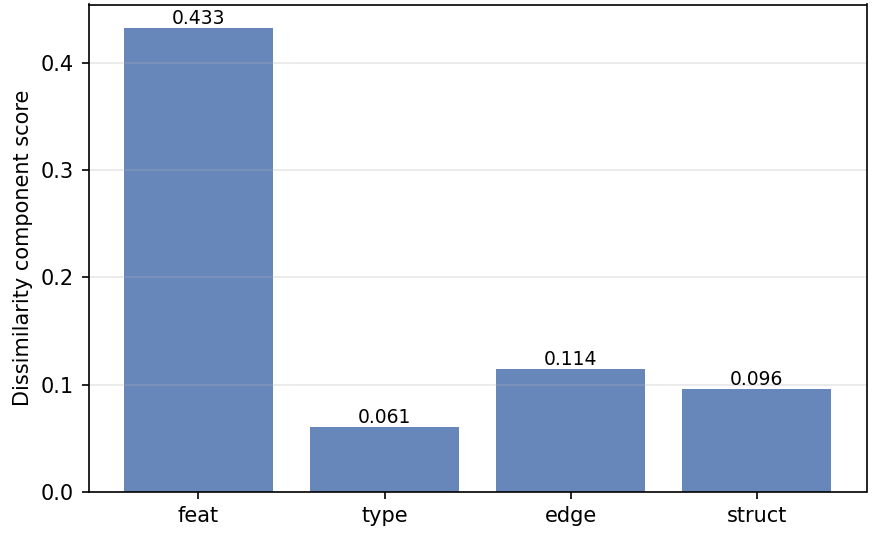
\includegraphics[width=1\textwidth]{figures/cf_showcase_dissimilarity_breakdown.png}
            \caption{Graph representation of the dissimilarity values for the distinct elements compared between the user's chosen graph and the chosen counterfactual.}
            \label{fig:cf_dissim_breakdown}
        \end{figure}
            
        My proposed counterfactual explanation relies on selecting a graph (graph 1), shown in Fig. \ref{fig:cf_query_graph}, that the stakeholder wishes to obtain an explanation for and then finding the most similar graph (graph 2) in the existing set that satisfies a given condition. This condition depends on the chosen KPI, in the case of this thesis the condition is that graph 2's remaining time prediction is lower than the remaining time predicted for the graph 1. Fig. \ref{fig:cf_dissim_breakdown} shows the result of this method. The dissimilarity score for the counterfactual subgraph against the input is shown to the stakeholder broken down between 4 bar graphs, each showing a different value of the total dissimilarity value. The goal of this graph is for the end user to easily identify the graph element that is driving the difference between the two similar graphs. Fig. \ref{fig:cf_dissim_breakdown} shows an example where the dissimilarity is mainly driven by the difference in features between the two subgraphs. 
        
        The stakeholder can define the minimum threshold value for the difference in prediction value between the subgraphs. In this example no minimum threshold was enforced (the default value of 0 hours was used), so the candidate set simply consists of the most similar graphs among those with a lower predicted remaining time. As can be seen in Fig. \ref{fig:cf_graph}, the identified counterfactual graph happens to have a total predicted time well below the query graph's (31.4 hours versus the query graph's 125.8) while also maintaining a similar overall structure. As was explained in Section \ref{sec:model_counterfactual} the chosen counterfactual subgraph is chosen from among a set of candidates identified as having a similar structure to the input graph. Fig. \ref{fig:cf_candidates} shows a table that is also provided to the stakeholder which shows the other two most similar graphs present in the candidates set and their dissimilarity values. 

        \begin{figure}[t!]
            \centering
            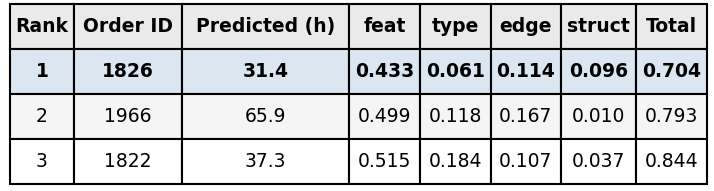
\includegraphics[width=1\textwidth]{figures/cf_showcase_candidates_table.png}
            \caption{Table showing the other possible counterfactual graph candidates found in the candidate set with their prediction value and dissimilarity scores}
            \label{fig:cf_candidates}
        \end{figure}
        
        In order to provide the stakeholder with a more actionable way of interpreting this explanation the different elements evaluated for the dissimilarity score are also shown in their own dedicated tables, highlighting the differences between them in the two subgraphs. For example, Fig. \ref{fig:cf_vwpnt_diff} and Fig. \ref{fig:cf_event_diff} show the difference in feature values between the Orders node and the Event nodes of the subgraphs respectively. Given that the dissimilarity was mainly driven by differences in features those different features are identified in this tables and shown to the stakeholder so they may better understand what's driving the model's predictions. 

        \begin{figure}[t!]
            \centering
            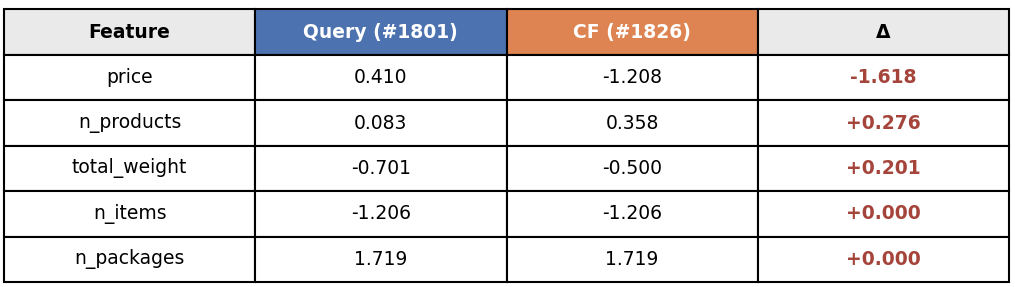
\includegraphics[width=1\textwidth]{figures/cf_showcase_viewpoint_feature_diff.png}
            \caption{Table showing the differences in the features of the Orders node of the two subgraphs. The total delta of the values is shown in the final column.}
            \label{fig:cf_vwpnt_diff}
        \end{figure}

        \begin{figure}[t!]
            \centering
            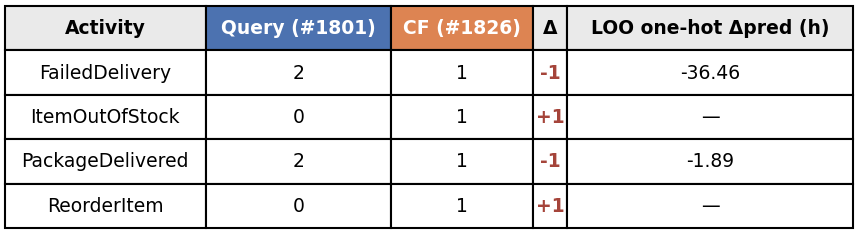
\includegraphics[width=1\textwidth]{figures/cf_showcase_event_type_diff.png}
            \caption{Table showing the differences in the features of the Event nodes of the two subgraphs. The number of events of each type is shown for the designated graph along with an estimation of their impact on the model's prediction.}
            \label{fig:cf_event_diff}
        \end{figure}

    \subsection{Explanation metrics}
        \begin{figure}[t!]
            \centering
            
\includegraphics[width=1\textwidth]{figures/explanation_quality_showcase_graphs.png}
            \caption{Graphs showing the baseline (full graph), fidelity+ (explanation removed), and fidelity- (explanation only) subgraphs used to compute the fidelity metrics meant for the stakeholder.}
            \label{fig:fidelity_graph}
        \end{figure}

        Finally, the stakeholder is also provided with fidelity metrics meant to help them assess the faithfulness of the explanation provided. An explanation is generated for the full graph using the framework and then the model's prediction is checked on a subgraph which does not contain the explanation subgraph (fidelity +) followed by a prediction performed on only the explanation subgraph (fidelity -). Fig. \ref{fig:fidelity_graph} shows the resulting baseline, fidelity+, and fidelity- graphs for one worked example, continuing the same order 1801 running example introduced earlier in this chapter. The stakeholder is shown only the resulting values for the given metrics, along with a short interpretation of the metric to aid them in their interpretation. Fig. \ref{fig:fidelity_table} shows the table of metrics. In this example the proposed explanation has a characterization score of 0.565 -- below the 0.815 aggregate LOO characterization reported for Order Management (Fig. \ref{fig:loo_comparison}) -- indicating that, while the proposed explanation is able to identify some of the input's most impactful elements, this particular trace is a comparatively less faithful case rather than the typical one. Its node sparsity value of 64.5\% and edge sparsity of 97.6\% indicate that the explanation has disregarded more than half of the existing nodes and almost all edges as unimportant to the model's prediction providing a very compact explanation subgraph.

        \begin{figure}[t!]
            \centering
            
\includegraphics[width=1\textwidth]{figures/explanation_quality_showcase_metrics_table.png}
            \caption{Table of the explanation metrics obtained.}
            \label{fig:fidelity_table}
        \end{figure}
    %!TEX root = ../dissertation.tex

\chapter{Conclusion}
\label{chp:conclusion}

This thesis aimed to address the problem of explainability applied to predictive process monitoring on object-centric event logs. As predictive process monitoring methods become more and more widespread, the reliance of these methods on black-box predictive models such as neural networks may be a detriment for user adoption since research has shown that process stakeholders will only adopt methodologies they feel they can trust. An explainability layer on top of these models can help create trust by providing insight into the elements driving a model's predictions. The proposal is a four-component explainability framework meant to provide stakeholders with clear and understandable insights into the predictive model being used. By providing both factual and counterfactual explanations, the stakeholder is able to understand which specific elements in their inputs are driving the model's prediction as well as how changing different elements in the input can lead to other desired outputs.


In order to test the framework two different synthetic OCEL 2.0 datasets are used, meant to emulate the processes of an Order Management and a Logistics company. For each dataset one heterogeneous graph neural network was trained per KPI, and two KPIs were chosen per dataset. The results show that, across the entire prefix set, the heterogeneous architecture is roughly on par with a homogeneous graph-based predictor, with overlapping confidence intervals across all four KPIs and no consistent winner. However, when compared only on last-event cases (which contain the greatest possible amount of information regarding a process execution) the picture becomes clearer. In these cases the heterogeneous model significantly outperformed every baseline on two of the four KPIs (Logistics' Depart and LoadToVehicle), remained the strongest choice but was statistically indistinguishable from the k-dim GNN baseline on a third (Order Management's PayOrder), and underperformed on the fourth (Order Management's PackageDelivered). This shows that the heterogeneous architecture is able to take advantage of richer input information as a process extends, though the benefit is KPI-dependent rather than universal.


The proposed explainability framework was then applied to all four KPI-specific regression models. The experimental evaluation showed that LOO analysis could be used as an efficient way of identifying impactful elements within the input graph, helping to curtail the number of elements for which the computationally costly Shapley Values analysis could be performed on. Similarly, gradient-based methods can be used to calculate the attribution value of element features in the graph and identify the most impactful elements on the model's prediction. Using these two identifier methods and applying Shapley Values to their chosen elements helped to provide a comprehensive set of input elements and the magnitude of their impact on the model's prediction. These results are then presented to the stakeholder in easy to understand graphs and tables that provide a clear look at the important elements, their rankings and their impact on the given prediction. In order to further create trust in the stakeholder, assessment metrics are also provided for the given factual explanations. Characterization and sparsity are shown to help the stakeholder understand how well the given explanation is at identifying the important elements for the model and separating them from the less important features.


Aside from giving insights into the particular elements driving the prediction, the framework is also able to provide the stakeholder with a counterfactual explanation method to help identify changes in the process that can lead to a desired change such as reducing the time remaining until an event occurs. By presenting these elements in a visually concise way, the stakeholder is able to identify key features in the process that can lead to reductions in the time it takes for a process to finish, or elements that are hindering the process as a whole.


Current limitations for the explainability framework pertain to the limited amount of explainability options available for use with heterogeneous models. While methods like HGExplainer and HTGExplainer exist, they could not be applied in this thesis given certain limitations (specifically for link-prediction/recommender-systems tasks and a failed port from DGL into PyTorch respectively). Additionally, while Shapley Values offer a comprehensive analysis of the features in a graph input and their impact on the prediction it also has a high computational cost which limits its possible applications as process executions grow in size and complexity. A further limitation observed during evaluation concerns the sensitivity of small temporal train/validation/test splits to whichever particular slice of a process's timeline each split happens to cover. For example, for one KPI (Order Management's "Orders to PayOrder"), the validation split's target values were found to be intrinsically less variable than the training split's, which on its own is enough to produce a pattern that could otherwise be mistaken for overfitting. Future work using a validation scheme less sensitive to which particular window of time it draws from, such as rolling-origin or k-fold temporal validation rather than a single fixed split, could mitigate this.


Future work in this space could seek to apply a similar explanation to a global, cross-trace view of the process rather than the current local-only implementation, following the work of de Leoni \& Volpato \cite{deleonieVolpato}. Similarly, a method seeking to use HTGExplainer could be constructed following a DGL-pipeline in order to validate its use on predictive process monitoring \cite{li2023}.


Ultimately, the proposed framework is able to provide insights into the predictive process monitoring model being applied to object-centric event logs. By providing stakeholders with explanations quantifying the impact of the most important elements of the inputs, metrics that assess the effectiveness of those explanations, and a counterfactual method to compare two distinct process executions, the framework provides a comprehensive look at the driving forces behind the predictive model.
    
    % afterword
    \cleardoublepage
    \phantomsection
    \addcontentsline{toc}{chapter}{References}
    \bibliography{references.bib}
    
    \cleardoublepage
    \phantomsection
    \addcontentsline{toc}{chapter}{Acknowledgments}
    \acknowledgments

\end{document}
